\documentclass[preprint, 3p,
authoryear]{elsarticle} %review=doublespace preprint=single 5p=2 column
%%% Begin My package additions %%%%%%%%%%%%%%%%%%%

\usepackage[hyphens]{url}

  \journal{Structural Change and Economic Dynamics} % Sets Journal name

\usepackage{graphicx}
%%%%%%%%%%%%%%%% end my additions to header

\usepackage[T1]{fontenc}
\usepackage{lmodern}
\usepackage{amssymb,amsmath}
% TODO: Currently lineno needs to be loaded after amsmath because of conflict
% https://github.com/latex-lineno/lineno/issues/5
\usepackage{lineno} % add
\usepackage{ifxetex,ifluatex}
\usepackage{fixltx2e} % provides \textsubscript
% use upquote if available, for straight quotes in verbatim environments
\IfFileExists{upquote.sty}{\usepackage{upquote}}{}
\ifnum 0\ifxetex 1\fi\ifluatex 1\fi=0 % if pdftex
  \usepackage[utf8]{inputenc}
\else % if luatex or xelatex
  \usepackage{fontspec}
  \ifxetex
    \usepackage{xltxtra,xunicode}
  \fi
  \defaultfontfeatures{Mapping=tex-text,Scale=MatchLowercase}
  \newcommand{\euro}{€}
\fi
% use microtype if available
\IfFileExists{microtype.sty}{\usepackage{microtype}}{}
\usepackage[]{natbib}
\bibliographystyle{elsarticle-harv}

\ifxetex
  \usepackage[setpagesize=false, % page size defined by xetex
              unicode=false, % unicode breaks when used with xetex
              xetex]{hyperref}
\else
  \usepackage[unicode=true]{hyperref}
\fi
\hypersetup{breaklinks=true,
            bookmarks=true,
            pdfauthor={},
            pdftitle={Exploring the forecasting and temporal causality patterns of multilayer trade networks reflecting global economic changes},
            colorlinks=false,
            urlcolor=blue,
            linkcolor=magenta,
            pdfborder={0 0 0}}

\setcounter{secnumdepth}{5}
% Pandoc toggle for numbering sections (defaults to be off)


% tightlist command for lists without linebreak
\providecommand{\tightlist}{%
  \setlength{\itemsep}{0pt}\setlength{\parskip}{0pt}}




\usepackage{float}
\usepackage{subfig}
\usepackage{graphicx}
\usepackage[utf8]{inputenc}
\usepackage{booktabs}
\usepackage{appendix}
\usepackage{hyperref}
\hypersetup{colorlinks=true,linkcolor=blue,filecolor=magenta,urlcolor=cyan,citecolor=blue}
\let\<\textless
\let\>\textgreater
\usepackage[para,online,flushleft]{threeparttable}
\usepackage{glossaries}
\newacronym{acf}{ACF}{Autocorrelation Function}
\newacronym{adf}{ADF}{Augmented Dickey-Fuller}
\newacronym{aic}{AIC}{Akaike Information Criterion}
\newacronym{ale}{ALE}{Average Local Efficiency}
\newacronym{arima}{ARIMA}{Autoregressive Integrated Moving Average}
\newacronym{assort}{Assort}{Assortativity}
\newacronym{aut}{AUT}{Authority Centrality}
\newacronym{avpl}{AVPL}{Average Path Length}
\newacronym{bc}{BC}{Betweenness Centrality}
\newacronym{bfa}{BFA}{Bayesian Factor Approach}
\newacronym{bic}{BIC}{Bayesian Information Criterion}
\newacronym{bvar}{BVAR}{Bayesian Vector Autoregression}
\newacronym{bz}{BZ}{Betweenness Centralization}
\newacronym{cc}{CC}{Closeness Centrality}
\newacronym{cz}{CZ}{Closeness Centralication}
\newacronym{dc}{DC}{Degree Centrality}
\newacronym{dens}{Dens}{Density}
\newacronym{dz}{DZ}{Degree Centralization}
\newacronym{dci}{DCI}{Indegree Centrality}
\newacronym{dzi}{DZI}{Indegree Centralization}
\newacronym{dco}{DCO}{Outdegree Centrality}
\newacronym{dmn}{DMN}{Dynamic Multilayer Network}
\newacronym{dzo}{DZO}{Outdegree Centralization}
\newacronym{ec}{EC}{Eigenvector Centrality}
\newacronym{ergm}{ERGM}{Exponential Random Graph Model}
\newacronym{es}{ES}{Edge Similarity}
\newacronym{ez}{EZ}{Eigenvector centralization}
\newacronym{fd}{FD}{Final Demand}
\newacronym{fevd}{FEVD}{Forecast Error Variance Decomposition}
\newacronym{gvc}{GVC}{Global Value Chain}
\newacronym{gle}{GLE}{Global Efficiency}
\newacronym{gnda}{GNDA}{Generalized Network-based Dimensionality Analysis}
\newacronym{gnn}{GNN}{Graph Neural Network}
\newacronym{hom}{HOM}{Homophily}
\newacronym{hub}{HUB}{Hubness Centrality}
\newacronym{hc}{HC}{Harmonic Centrality}
\newacronym{ibbig}{iBBiG}{iterative Binary Biclustering of Gene sets}
\newacronym{icio}{ICIO}{Inter-Country Input-Output}
\newacronym{ict}{ICT}{Information and Communications Technology}
\newacronym{mcmc}{MCMC}{Markov Chain Monte Carlo}
\newacronym{mlavpl}{MLAVPL}{Multilayer Average Path Length}
\newacronym{mlglclu}{MlGlClu}{Multilayer Global Clustering Coefficient}
\newacronym{mod}{Mod}{Modularity}
\newacronym{mva}{MVA}{Mean of Vertex Asymmetries}
\newacronym{ns}{NS}{Node Similarity}
\newacronym{pacf}{PACF}{Partial Autocorrelation Function}
\newacronym{oecd}{OECD}{Organisation for Economic Co-operation and Development}
\newacronym{pd}{PD}{Pearson Correlation of Degree Centralities}
\newacronym{prc}{PRC}{PagRank Centrality}
\newacronym{prz}{PRZ}{PagRank Centralization}
\newacronym{rcc}{RCC}{Reach Club Coefficient}
\newacronym{rres}{RRes}{Random Resiliency}
\newacronym{rw}{RW}{Random Walk}
\newacronym{sc}{SC}{Schwarz Criterion}
\newacronym{sci}{SCI}{Instrength Centrality}
\newacronym{sco}{SCO}{Outstrength Centrality}
\newacronym{sp}{SP}{Shortest Path Distance}
\newacronym{sres}{SRes}{Systematic Resiliency}
\newacronym{trans}{Trans}{Transitivity}
\newacronym{va}{VA}{Value Added}
\newacronym{var}{VAR}{Vector Autoregressive}
\newacronym{wto}{WTO}{World Trade Organization}
\makeglossaries
\usepackage{color}
\usepackage[table,xcdraw]{xcolor}
\newcommand{\darkred}[1]{\color{red!50!black}{#1}\color{black}}
\newcommand{\darkgreen}[1]{\color{green!50!black}{#1}\color{black}}
\newcommand{\darkblue}[1]{\color{blue!50!black}{#1}\color{black}}
\usepackage{booktabs}
\usepackage{longtable}
\usepackage{array}
\usepackage{multirow}
\usepackage{wrapfig}
\usepackage{float}
\usepackage{colortbl}
\usepackage{pdflscape}
\usepackage{tabu}
\usepackage{threeparttable}
\usepackage{threeparttablex}
\usepackage[normalem]{ulem}
\usepackage{makecell}
\usepackage{xcolor}



\begin{document}


\begin{frontmatter}

  \title{Exploring the forecasting and temporal causality patterns of
multilayer trade networks reflecting global economic changes}
    \author[Department of Quantitative Methods, University of
Pannonia]{Zsolt T. Kosztyán%
  %
  }
   \ead{kosztyan.zsolt@gtk.uni-pannon.hu} 
      \cortext[cor1]{Corresponding author}
  
  \begin{abstract}
  This study examines the dynamic evolution of global trade networks
  from 1995 to 2020 using the Organisation for Economic Co-operation and
  Development's (OECD's) intercountry input--output (ICIO) data. This
  research combines multilayer network theory methods with advanced
  statistical and econometric procedures, including dynamic multilayer
  network analysis methods, (bi)clustering, and causal analyses to
  evaluate the temporal nature of structural, sectorial and
  country-level indicators. The primary objective of this study is to
  identify causal patterns in multilayer trade network structures and
  reveal the roles of specific countries and industries as drivers of
  changes in global trade dynamics. Using the proposed methods, we
  define causal graphs between the structural indicators of the
  multilayer network. The resulting causal graph is organized into
  groups using modularity analysis, and the relationships are
  biclustered, thereby determining which structural
  factors/industries/countries affect other country groups/industries
  and revealing the dynamics of structural changes. We determine which
  factors change simultaneously and which factors and actors exhibit a
  delay between their changes. The analysis reveals significant shifts
  in structural indicators, highlighting the evolving roles of major
  players like China and the US. The findings indicate that the
  structural indicators of trade networks / industries/countries often
  move in unison, with changes in one country/industry potentially
  triggering rapid transformations across the entire network. This study
  also uncovers the cascading effects of economic disruptions on trade
  patterns, emphasizing the interconnectedness of countries and
  industries in the face of global economic changes. These insights are
  crucial for policymakers and business leaders, underscoring the need
  for adaptive strategies to enhance the level of resilience of
  countries and industries to persistent global economic fluctuations
  and crises.
  \end{abstract}
    \begin{keyword}
    multilayer trade networks \sep causality analysis \sep global
changes \sep 
    temporal patterns
  \end{keyword}
  
 \end{frontmatter}

\sloppy

\section{Introduction}\label{introduction}

At the same time as this study was submitted, the US administration
announced a large increase in tariffs, with which they intend to bring
in a new era in world trade; thus, this study, which aims to explore the
actors, industries, and structural relationships of global trade, could
perhaps not be timelier. Examining the structural changes in trade
networks \citep{james2001, he2010structure, guo2023impact} -- especially
now, in this rapidly changing economic environment -- is essential, as
these changes frequently reflect wider economic and social transitions
within the economy and society
\citep{stolte2021structural, mahutga2006persistence}. Shifts in trade
patterns may indicate changes in consumer preferences
\citep{janeba2007international}, technical progress
\citep{guerrieri1999technology, yi2021structural}, the rise of new
markets \citep{antonelli2002microdynamics, alamsyah2023rise}, or
geopolitical realignments \citep{barbieri2024geopolitics}, thereby
impacting local economies and global market dynamics
\citep{paolo2022, antonelli2002microdynamics}. Furthermore, examining
these alterations may reveal power transitions among countries
\citep{li2024evolutionary}, which can both be a consequence of political
and economic decisions \citep{kosztyan2024trade} and influence further
political decisions \citep{milner2017political}, and highlight the
interdependence of economies in a progressively globalized environment
\citep{kosztyan2024trade}. Comprehending these structural alterations
not only assists in forecasting future economic trends but also enables
the recognition of the weaknesses and opportunities within trade systems
\citep{sun2022influence}, thus enhancing strategic decision-making and
promoting sustainable development \citep{xu2025evolution}.

Recent literature has emphasized the importance of examining trade
networks through various lenses
\citep{xu2025evolution, li2024evolutionary}. Focusing on actual policy
changes and their consequences \citep{kosztyan2024trade}, rather than
hypothetical scenarios, offers a more accurate reflection of trade
policy impacts on economic outcomes
\citep{pinelopi2016, ortiz2021review}. \citet{he2010structure} and
\citet{guo2023impact} highlighted the importance of investigating
structural changes in trade networks, while \citet{stolte2021structural}
and \citet{mahutga2006persistence} explored how these changes reflect
wider economic and social transitions and political decisions
\citep{kosztyan2024trade}. \citet{janeba2007international} focused on
the role of consumer preferences in shaping trade patterns, and
\citet{antonelli2002microdynamics} examined the impact of technological
progress and new market emergence on global market dynamics. More recent
studies, such as \citet{li2024evolutionary}, have delved into power
transitions among countries, with \citet{kosztyan2024trade} dealing with
the structural changes in trade networks caused by political and
economic decisions and crises.

Despite the wealth of research in this area, significant gaps in our
understand the causal patterns within trade network structures and the
identification of key drivers of change among countries and sectors
remain. Traditional methods have often focused on static analyses or
limited time frames, failing to capture the dynamic nature of trade
relationships and their evolution over extended periods. There is a call
for more sophisticated methodologies that can explore complex interplay
among the economic, political, and social factors driving trade network
dynamics. Additionally, many studies have focused only on single-layer
networks and have not fully explored the multilayered nature of trade
networks, which can provide deeper insights into the complex
interactions between different industries and countries.

To address these gaps, this study employs advanced methodologies
including the temporal analysis of multilayer networks, clustering,
biclustering, and causality analysis. These methods enable the dynamic
and causal analysis of structural indicators at the structural, country
and industry levels. By utilizing these techniques, we can explore the
interplay between industries and countries' trade relations, which is
particularly relevant to the eve of the imminent trade war at the time
of writing this paper. This approach is particularly important in the
context of persistent global economic fluctuations and crises, as we can
gain a deeper understanding of how economic disruptions affect trade
relations and network structure, which can inform more effective
policymaking and business strategies to enhance the degree of resilience
to future challenges.

The main research question of our study is as follows:

\begin{description}
\item[RQ\label{rq}] What causal patterns can be identified in multilayer trade network structures, and how do these patterns reveal the roles of specific countries and industries as drivers of change in global trade dynamics?
\end{description}

The methodological framework employed in this study is grounded in
established theoretical principles for causal identification in
multidimensional interactive systems, particularly those involving
simultaneous country-industry-structural attribute dependencies. Granger
causality testing provides a theoretically sound approach for
disentangling temporal precedence relationships in complex economic
networks where simultaneity bias and reverse causality are prominent
concerns \citep{hamilton2020time}. Recent advances in network
econometrics demonstrate that Granger causality, when applied to
structural network indicators, effectively captures propagation
mechanisms in multilayered systems where traditional instrumental
variable approaches fail due to the absence of valid exclusion
restrictions \citep{siggiridou2019evaluation}. The integration of
Bayesian validation methods (\gls{bvar}, \gls{mcmc} analysis, \gls{bfa})
addresses the fundamental challenge of parameter uncertainty in finite
samples, which is particularly relevant for trade network analysis where
structural breaks and nonlinearities can confound classical inference
\citep{koop1996impulse, celani2024bayesian}. Biclustering methodology
complements causality analysis by simultaneously identifying groups of
causal relationships and network nodes that exhibit coherent temporal
patterns, addressing the curse of dimensionality inherent in
multi-country, multi-industry systems \citep{g2024comprehensive}. This
methodological combination is theoretically justified because trade
networks exhibit what \citet{carvalho2013great} term ``granular origins
of aggregate fluctuations,'' where microlevel (country-industry) shocks
propagate through network structures to generate macrolevel patterns,
requiring both temporal precedence identification (Granger causality)
and structural pattern recognition (biclustering) to fully characterize
the transmission mechanisms; however, to the best of our knowledge these
methods are not used together.

\section{Background}\label{background}

In the current economic environment, especially at the beginning of
another tariff war, it is particularly important to understand the
dynamics of trade networks, that is, the interaction of actors and
industries. The evolution of network science, boosted by the
accessibility of vast datasets and improved processing capabilities, has
revolutionized how academics and practitioners study complicated systems
such as trade networks \citep{xu2025evolution}. The volatility of trade
arising from political conflicts, economic crises, and health
emergencies has underscored the interconnectedness among trade
relationships and their effects on economic stability \citep{Xiang2013}.
While individual countries struggle with the consequences of such
disruptions, trying to take countermeasures to reduce these effects,
these measures are quite limited due to the interconnectedness of trade
networks \citep{Zhao2024}. The increased degree of interdependence of
countries in the global trade environment has amplified the possibility
of failure propagation across international trade networks
\citep{Kang2024}.

Research on the time-series analysis of trade networks has employed
predominantly dynamic network theory to examine trade relationships over
time \citep{Yazawa2023}. However, very few studies have addressed the
causal investigation of the structural characteristics of trade networks
or the exploration of impact mechanisms. Forecasting has been applied
using \gls{icio} \citep{chen2024prediction}. These approaches have been
instrumental in identifying the key drivers of trade network evolution
and predicting future trade patterns \citep{chen2024prediction}.

While network analysis has been extensively used, causality analysis
within trade networks has been less common but not entirely absent.
Granger causality tests and vector autoregression models have been
employed to determine the causal relationships between different
countries' economic activities, providing insights into how changes in
one country can influence the trade dynamics of other countries
\citep{Saimul2020}. One study has utilized \glspl{gnn} to model causal
relationships in trade networks \citep{monken2021graph}, particularly in
response to major economic events such as trade wars or financial
crises. Causal inference techniques have also been explored to
understand how external shocks propagate through trade relationships;
offering a deeper perspective on economic dependencies
\citep{rigena2021}. However, to our knowledge, no study has explored the
causal relationships and mechanisms of effects among countries,
industries, and structural properties of the network. Furthermore,
biclustering methods have not yet been applied in commercial networks,
although combining this method with causality analysis makes it possible
to determine close causal groups that simultaneously affect other
factors. Biclustering \citep{g2024comprehensive} can allow for the
identification of subgroups of countries and industries with similar
trade behaviors, revealing hidden trade patterns and dependencies. This
approach could improve our understanding of how trade clusters respond
to global shocks, aiding policymakers in optimizing trade agreements.
Investigating biclustering in trade networks would enhance the
analytical depth beyond traditional clustering methods, potentially
uncovering new strategic trade insights.

Recent network-based approaches to international trade and \glspl{gvc}
have mapped the architecture of globalization and documented salient
topological regularities, but typically in single-layer or
sector-specific settings \citep{liu2025spatial}.
\citet{kali2007architecture} that a country's structural position in the
global trade network--beyond trade volumes--matters for growth, yet
their analysis is single-layer and relies on two cross-sections (1992,
1998), without modeling temporal causality among structural indicators
\citep{kali2007architecture}. \citet{cerina2015world} construct the
World Input--Output Network is used to characterize the large-scale
topology, providing an important benchmark for system-wide structure but
not a multilayer, temporal causal analysis \citep{cerina2015world}. More
recently, \citet{piccardi2024patterns} introduce a network-based measure
of \gls{gvc} ``length,'' revealing heterogeneous, geography-sensitive
adjustments in global value networks; however, their focus is on
measuring extension and communicability rather than forecasting or
identifying temporal precedence among network indicators
\citep{piccardi2024patterns}. Sectoral contributions, such as analysis
by \citet{russo2023regionalisation} of automotive multilayer clusters,
uncover twin dynamics of regionalization and cross-region integration,
but remain industry-focused and descriptive with respect to network
evolution and inter-indicator causality
\citep{russo2023regionalisation}. Complementing these strands, the
survey by \citet{amador2016global} synthesizes drivers and measures of
\glspl{gvc} but does not prescribe a multilayer, time-ordered causal
modeling framework \citep{amador2016global}.

Our study advances this literature along four fronts. First, we build a
dynamic, multilayer network from \gls{oecd} \gls{icio} data at the
country--industry level over a long horizon (1995--2020), enabling
system-wide, cross-sector generality beyond single-sector or
short-window analyses
\citep[cf.][]{russo2023regionalisation, piccardi2024patterns}. Second,
we move from descriptive topology to mechanisms by applying temporal
(classical and Bayesian Granger and instantaneous) causality tests to
structural indicators across layers, thereby identifying drivers and
propagation pathways among countries, industries, and network
properties--an aspect not addressed by the above works. Third, we
operationalize structure-based forecasting of network indicators
(out-of-sample, 2021--2030), which extends prior contributions centered
on static maps, length metrics, or cluster detection
\citep{kali2007architecture, cerina2015world, russo2023regionalisation}.
Fourth, by combining dynamic multilayer analysis with modularity-based
grouping and biclustering, we detect coherent, co-moving causal groups
of indicators and country--industry nodes, providing a decision-oriented
decomposition of systemic change that complements survey-based
measurement frameworks \citep{amador2016global}. Together, these
features position the paper as a bridge between topology, temporal
causality, and predictive analytics in multilayer \gls{gvc} networks.

Building on the literature, the following contributions are made:

\begin{description}
\item[C$_1$\label{c1}] Revealing the dynamic evolution of the global trade network structure and its catalysts for change.
\item[C$_2$\label{c2}] Disclosing the cascading impacts of trade interconnectedness and disruptions on international trade connections among nations and sectors.
\item[C$_3$\label{c3}] Identifying intervention points for decision-makers, helping contain potential escalations and mitigating the disruption caused by crises.
\end{description}

We study multilayer trade networks (country \(\times\) industry
\(\times\) time), which capture cross-industry interdependencies more
fully than single-layer representations. (\nameref{c2}). This approach
enables researchers to examine how changes in one sector or country can
ripple through various layers of the trade network, providing a more
realistic representation of the intricate global economic mechanism
(\nameref{c1}). The multilayer structure also facilitates the
identification of hidden patterns and relationships that may not be
apparent when individual layers in isolation are being examined. This
enhanced analytical capability is particularly valuable for
understanding the cascading effects of economic disruptions and policy
changes across sectors and nations, ultimately leading to more informed
decision-making in international trade policies and strategies
(\nameref{c3}).

\section{Data and Methods}\label{data-and-methods}

We examined the \gls{oecd} \gls{icio} multilayer trade network between
1995 and 2020. We calculated the temporal evolution of structural
network-, industry- and country-level node indicators on the multilayer
network during this period. We determined changes in the role of sectors
and countries over time and then used these to create time series to
examine forecasts and determine causal networks based on
cause-and-effect studies between indicators. We grouped the effects
using clustering and biclustering procedures. Our goal was to determine
which structural factors, which sectors and which countries are the
driving forces of the structural changes (see \nameref{rq}) and how to
map the temporal dynamics of these changes (see
\nameref{c1}-\nameref{c3}).

The research framework of this study is shown in Figure
\ref{fig:methods}.

\begin{figure}[H]
\caption{Research framework}
\label{fig:methods}
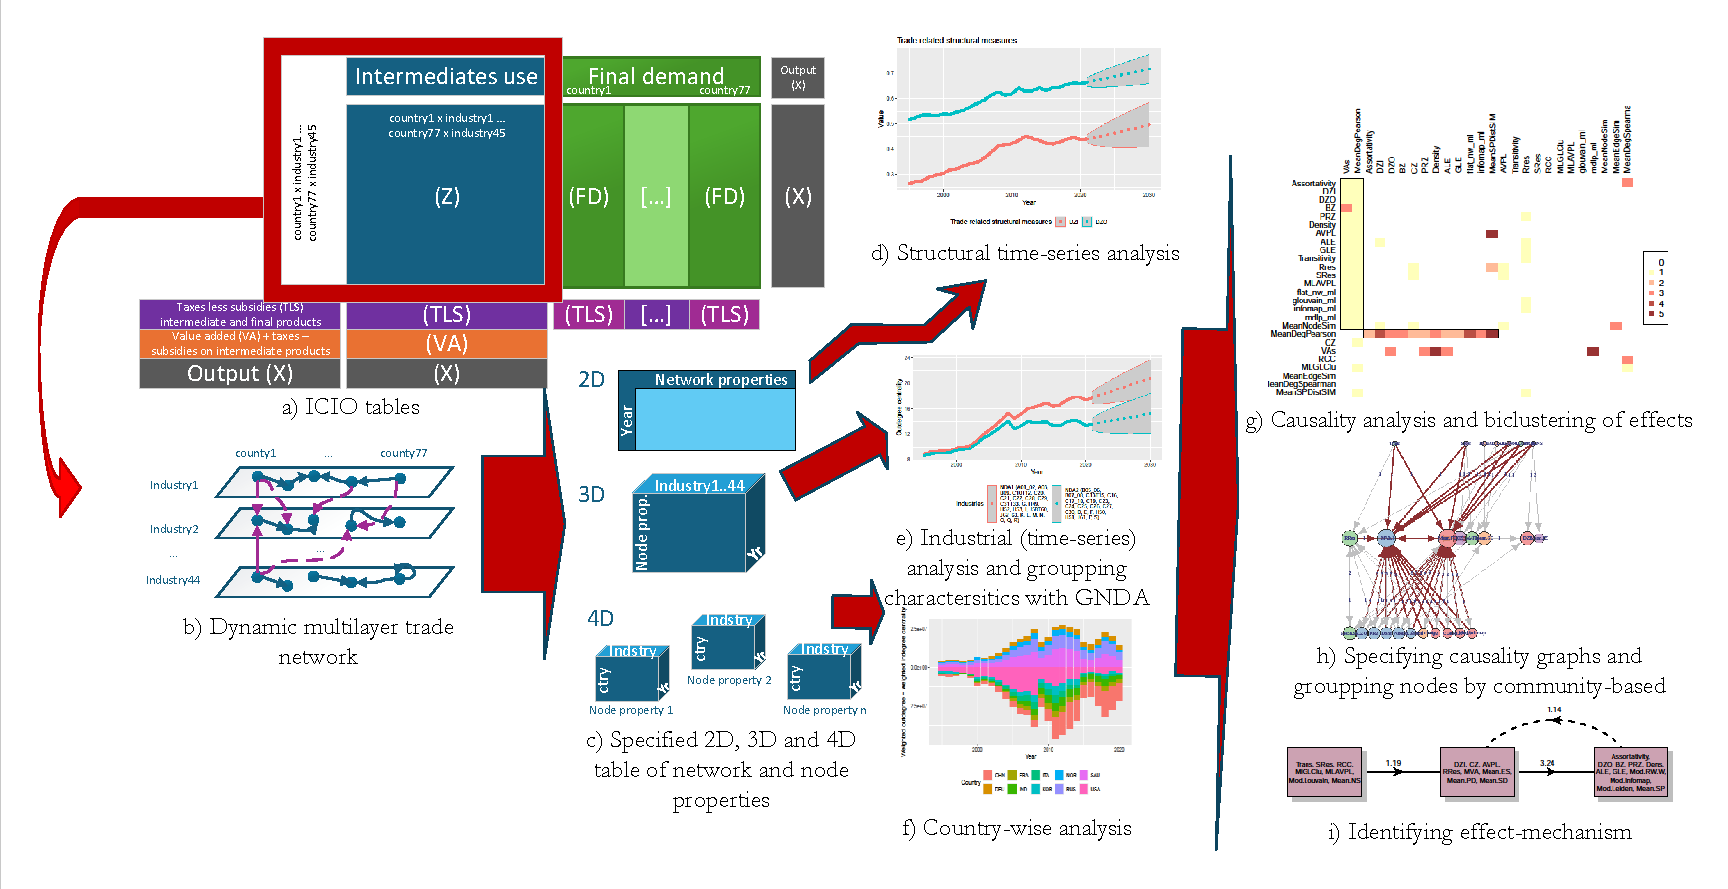
\includegraphics[width=\textwidth]{methods.pdf}
\end{figure}

\subsection{Employed Data}\label{employed-data}

The \gls{oecd}'s \gls{icio} tables (see Figure \ref{fig:methods}(a)) map
production, consumption, investment, and international trade in goods
and services. Economic activity and country are split into these tables
to show global economic linkages in detail. \gls{icio} tables have the
following main segments: intermediate use (Z): goods and services used
as inputs in other manufacturing, which shows industry and sector
interdependencies within and between countries. In our study, we
analyzed this segment in detail. \gls{fd} for goods and services in a
country, which include household consumption, government spending,
investment, and net exports, referencing economic goods and service
consumption. The total worth of an industry or sector's goods and
services is output (X), which covers intermediate use and FD. This
chapter shows the net effect of taxes and subsidies on production and
comprises indirect taxes such as value-added taxes (VATs) and government
subsidies to various industries. Value added (VA): an industry or sector
adding value to its intermediate inputs. The gap between output and
intermediate use represents the contribution of labor and capital to
production.

\subsubsection{Data Collection and
Preparation}\label{data-collection-and-preparation}

In this study, we used mainly the intermediate use (Z) segment to
construct a multilayer dynamic network, and examined its structure,
industry, and country-level changes. The edge list of the dynamic
multilayer data table, which served as the basis for the analysis, was
encoded as follows:

\begin{center}
Year | From.Sector | From.Country | To.Sector | To.Country | Value
\end{center}

Instead of country and industry codes, we used numbered IDs, and the
lists of country and sectorial codes are shown in Tables
\ref{tab:countries}-\ref{tab:industries}. An example of a data row is as
follows:

\begin{center}
1995 | 1 |1 | 1 | 2 | 8.5029
\end{center}

This means that in 1995, from country 1 (Argentina, ARG), the total
amount of trade to country 2 (Australia, AUS; see Table
\ref{tab:countries}), in sector 1 (agriculture, hunting and forestry,
A01\_02) was 8.5029 million USD. The employed data structure enabled us
to specify a \gls{dmn} (see Figure \ref{fig:methods}(b)).

To construct the 77 × 45 (countries × industries) dynamic panel, we
harmonized ICIO flows to the OECD 45-industry (ISIC Rev.4) aggregate
using the official concordances and the back-casted, balanced time
series that mitigate reclassifications and vintage breaks
\citep{oecd2020}. The residual share of missing entries was negligible;
accordingly, no ad-hoc imputation was applied. To improve robustness, we
excluded annual bilateral industry flows below USD 1 million, since very
small cells in multi-country IO tables are disproportionately affected
by confidentiality treatment, balancing residuals, and rounding noise.
This conservative sparsification removes negligible aggregate value but
materially improves the signal-to-noise ratio for temporal forecasting
and causality analysis, while preserving temporal comparability where
\gls{oecd} flags structural breaks.

We extend the dynamic multilayer network with two additional \gls{icio}
blocks. (i) The value-added (VA) matrix, available as Year \(\times\)
(Country \(\times\) Industry), is modeled as an ``income'' layer in
where each country-industry node directs its value added to a synthetic
Domestic-Income node of its own country. (ii) The Final-Demand (FD)
tensor (Year \(\times\) (Country \(\times\) Industry) \(\times\)
Final-User Country) constitutes a ``demand'' layer whose edges run from
producing country-industry nodes to final consumer countries. Together
with the intermediate-use (Z) layer, which yields a three-layer
Supply--Demand--Income multiplex observed from 1995 to 2020. All network
and node indicators are computed for each layer separately, allowing
straightforward robustness checks of Z-based results against FD and VA
perspectives.

\subsubsection{Specification of Multidimensional Network- and Node-Level
Datasets}\label{specification-of-multidimensional-network--and-node-level-datasets}

After constructing the \gls{dmn}, we specified three types of datasets
for further examination. We calculated structural network properties for
each year. These results were stored in a 2D data table (see Figure
\ref{fig:methods}(c)), where the columns denote the calculated
structural properties of the network and the rows denoted the given
years. Utilizing the constructed table, we analyzed the structural
changes in the trade network. Similarly, a 3D data table was
constructed, where the dimensions were industries (sectors),
(aggregated) node indicators and years \ref{fig:methods}(e)). We also
created an aggregated data table for countries. The proposed 3D dataset
allows us to answer the following question: How much does the change in
the role of different industries depends on other industries and on what
extently do these characteristics move together? Finally, we created a
4D dataset, where the dimensions are country, industry, and node
property under study, and time (see Figure \ref{fig:methods}(f)). In
this case, we obtained answers to the question of how countries' trade
in different sectors changes over time.

\subsection{Employed Methods}\label{employed-methods}

To answer the research question posed (see \nameref{rq}), it was
necessary to employ several methods. First, we calculated the time
changes and forecasts in the network and node indicators of the dynamic
multilayer trade network (see Figure \ref{fig:methods}(d-f) and Section
\ref{sec:methodnetwp}). However, we grouped these factors to determine
which countries and sectors have similar structural indicators (see
Sections \ref{sec:simnet} and \ref{sec:methodnodep}). We then analyzed
the time series obtained for the network and node indicators using
Granger causality tests (see Figure \ref{fig:methods}(h) and Section
\ref{sec:methodcaus}). On the basis of the results of the causality
studies, we mapped the causal networks between both structural and
industrial and country-level indicators (see Figure
\ref{fig:methods}(h)). We grouped the relationships by biclustering
procedures (see Figure \ref{fig:methods}(g-h), while using module search
procedures, we identified those indicator groups with closer
relationships (see Figure \ref{fig:methods}(h) and Section
\ref{sec:clust}). Next, we determined the mechanisms of action between
the indicators (see Figure \ref{fig:methods}(i)).

\subsubsection{The representation of dynamic multilayer trade
network}\label{the-representation-of-dynamic-multilayer-trade-network}

A dynamic multilayer (trade) network is a triplet,
\(G(t)=(V(t),E(t),W(t))\), where vertices (\(V(t)\)) are organized into
multiple layers (\(L\)) in time \(t\in T\) and each node (vertex)
corresponds to an actor (\(A(t)\)), where the same actor at time \(t\)
can be mapped to nodes in different layers. Formally,
\(V(t) \subseteq A(t) \times L\). \(E(t) \subseteq V(t) \times V(t)\) is
set of undirected edges between two vertices at time \(t\).
\(W(t) : E(t) \rightarrow \mathbb{R}^+\) represents the weights of each
edges at time \(t\). A dynamic edge is represented as having the
following four members: \(e_{ip,jq}(t)=(a_i(t),l_p,a_j(t),l_q)\); the
weight of a dynamic edge is \(w(e_{ip,jq}(t)) \in \mathbb{R}^+\), where,
in this study, \(t\in T:=\{1995,\ldots,2020\}\), \(a_i,a_j\in A\) are
exporters (\(i\)), and importers (\(j\)) actor (i.e., country),
\(l_i,l_j\in L\) are the layers of exporters and importers,
respectively; \(c_{ip} =(a_i,l_p) \in V\) is the node, where
\(a_i \in A\) is the actor in layer \(l_p\in L\). If we fix the year of
\(t\), then we obtain a static multilayer trade network.

\subsubsection{Explored node-level properties}\label{sec:methodnodep}

The employed centrality measures can be calculated for each country in
all industrial layers and can be aggregated at the industrial or country
level. These indicators jointly offer an extensive perspective on the
roles and influences of many countries within the multilayered trade
network. Utilizing these indicators enables the analysis of countries'
interactions in trade, economic robustness, and strategic standing
within the global trade framework. The time-series analysis of these
indicators can reveal how the role of countries or sectors has evolved
over time. Table \ref{tab:nodeprop} in the Appendix shows the
mathematical formulation of the employed node-level indicators. Table
\ref{tab:node_indicators_economic} summarizes the economic insights the
employed node-level indicators.

\begin{table}[htp]
\centering
\caption{Node-level Indicators with Economic Interpretations}
\resizebox{\linewidth}{!}{
\begin{tabular}{p{0.15\textwidth} p{0.30\textwidth} p{0.75\textwidth}}
\hline
\textbf{Economic Dimension} & \textbf{Indicators} & \textbf{Economic Meaning and Interpretation} \\
\hline

\textbf{Market Access and Trade Diversification} & 
\begin{tabular}[t]{@{}l@{}}
\gls{dci}\\
\gls{dco}\\
\gls{dc}
\end{tabular} & 
Measures a country's trade relationship diversification and market access breadth. High \gls{dci} indicates strong import demand and supplier dependency, signaling domestic market attractiveness but potential vulnerability to supply disruptions. High \gls{dco} reflects robust export capacity and market penetration across multiple destinations, indicating competitive advantage and reduced dependency on single markets. Together, they reveal a country's integration into global supply chains and resilience through diversification. \\
\hline

\textbf{Economic Scale and Trade Volume} & 
\begin{tabular}[t]{@{}l@{}}
\gls{sci}\\
\gls{sco}
\end{tabular} & 
Captures a country's actual economic weight and trade intensity in global markets. High \gls{sci} represents substantial import dependency and domestic consumption capacity, indicating economic size but potential external vulnerability during supply chain disruptions. High \gls{sco} demonstrates export-oriented economic strength and international competitiveness, contributing to GDP growth and foreign exchange earnings. The difference (SCO-SCI) reveals trade balance dynamics, crucial for understanding current account sustainability and economic stability. \\
\hline

\textbf{Strategic Trade Position and Market Control} & 
\begin{tabular}[t]{@{}l@{}}
\gls{bc}\\
\gls{cc}
\end{tabular} & 
Measures a country's strategic importance in global trade routes and market accessibility. High \gls{bc} indicates critical intermediary role, enabling control over trade flows and potential for rent extraction through gateway positions. Countries with high \gls{bc} can influence global supply chains and may benefit from trade disruptions affecting competitors. High \gls{cc} ensures efficient access to diverse trading partners, reducing transaction costs and enhancing trade opportunities, particularly valuable during market volatility and crisis periods. \\
\hline

\textbf{Economic Influence and Network Power} & 
\begin{tabular}[t]{@{}l@{}}
\gls{ec}\\
\gls{prc}
\end{tabular} & 
Evaluates a country's influence by considering not just connection quantity but partner quality and importance. High values indicate trade relationships with economically powerful nations, enhancing technological spillovers, knowledge transfer, and economic stability through association with stable partners. This is particularly crucial for developing countries seeking technology transfer and for developed nations maintaining leadership in innovation networks. Such positions provide resilience during economic downturns through diversified high-quality partnerships. \\
\hline

\textbf{Hub Economy Functions} & 
\begin{tabular}[t]{@{}l@{}}
\gls{aut}\\
\gls{hub}
\end{tabular} & 
Measures a country's role as a trusted trade node in global commerce. High \gls{aut} signifies reputation as a reliable export destination, often associated with high-quality goods, advanced manufacturing, or specialized services, creating premium positioning and pricing power. High \gls{hub} indicates major exporter status to influential importers, suggesting critical supply chain importance and potential for economic leverage. Together, they identify countries that serve as essential connectors in global trade networks, with significant bargaining power and economic influence. \\
\hline

\textbf{Industrial Specialization and Risk Concentration} & 
\gls{hom} & 
Measures the percentage of a country's trade relationships within the same industry, revealing specialization patterns and associated risks. High homophily indicates strong industrial specialization and competitive advantage in specific sectors, potentially leading to higher productivity and export revenues. However, it also signals vulnerability to industry-specific shocks, technological disruptions, or demand shifts. Low homophily reflects diversified trade portfolios and risk management strategies, providing stability during sector-specific crises but potentially sacrificing specialization benefits and economies of scale. \\
\hline
\end{tabular}}
\label{tab:node_indicators_economic}
\end{table}

Our selection of node-level metrics is driven by economic relevance
rather than methodological exhaustiveness. Degree (in/out;
\gls{dci}/\gls{dco}) captures partner diversification -- the export
market access and redundancy versus procurement breadth and exposure --
while strength (out/in; \gls{sco}/\gls{sci}) measures realized trade
intensity and economic weight, with \gls{sco}--\gls{sci} informing
external balance and current-account sustainability. \gls{bc} quantifies
intermediation power over trade routes (gatekeeping, rerouting options,
rent extraction), and closeness (\gls{cc}) reflects the average market
access costs and speed of adjustment, key for resilience and price
pass-through. Eigenvector and PageRank (\gls{ec}/\gls{prc}) measure
embeddedness in ``high-quality'' neighborhoods -- the importance of
partners' partners -- linked to demand stability, technology spillovers,
and sanctions contagion. Hub/authority (\gls{hub}/\gls{aut})
disentangles upstream vs downstream roles in \glspl{gvc} (major
suppliers to influential buyers vs trusted destinations), informing
upgrading, reshoring, and supplier diversification strategies. Finally,
homophily (\gls{hom}) gauges specialization versus diversification in a
country--industry trade portfolio, balancing productivity gains against
sector-specific shock vulnerability. Table
\ref{tab:node_indicators_economic} synthesizes these economic
interpretations.

\subsubsection{Explored network-level properties}\label{sec:methodnetwp}

In addition to the aggregation of node-level indicators for industries
and the network, it is also possible to calculate network-level
indicators.

We calculate network centralization by first determining the centrality
values of each node. Afterward, we calculate the difference between the
highest centrality value and the centrality values of all the other
nodes. Finally, we sum these differences and divide them by the sum of
the maximum possible differences to obtain the centrality value of the
network. A formal description of network-level indicators are provided
in Table \ref{tab:netwprop} in the Appendix. The Table
\ref{tab:network_indicators_economic} shows a brief summary of the
economic insight into the employed network-level indicators.

\begin{table}[htbp]
\centering
\caption{Network-level Indicators with Economic Interpretations}
\resizebox{\linewidth}{!}{
\begin{tabular}{p{0.15\textwidth} p{0.32\textwidth} p{0.65\textwidth}}
\hline
\textbf{Economic Dimension} & \textbf{Indicators} & \textbf{Economic Meaning and Interpretation} \\
\hline

\textbf{Market Integration and Connectivity} & 
\begin{tabular}[t]{@{}l@{}}
\gls{dens}\\
\gls{avpl}\\
\multicolumn{1}{p{4cm}}{\gls{mlavpl}}
\end{tabular} & 
Measures the degree of global economic integration and trade efficiency. High density indicates tightly interconnected markets with extensive trade relationships, fostering collaboration and knowledge spillovers but potentially increasing systemic risk. Low \gls{avpl} suggests efficient trade routes and reduced transaction costs, enabling rapid price arbitrage and market equilibration. \gls{mlavpl} captures cross-industry connectivity, revealing how efficiently goods and services flow between sectors, crucial for understanding supply chain optimization and industrial interdependencies during economic shocks. \\
\hline

\textbf{Network Resilience and Stability} & 
\begin{tabular}[t]{@{}l@{}}
\gls{trans}\\
\gls{rres}\\
\gls{sres}
\end{tabular} & 
Evaluates the robustness of global trade networks against disruptions. High transitivity indicates clustering among trading partners, providing alternative trade routes and reducing vulnerability to single-point failures. This creates redundancy that protects against supply chain disruptions. Random resilience measures network stability against unexpected failures (natural disasters, political instability), while systematic resilience evaluates vulnerability to targeted attacks or coordinated disruptions (trade wars, sanctions). Together, they assess the global economy's capacity to maintain trade flows during various crisis scenarios. \\
\hline

\textbf{Trade Concentration and Market Power} & 
\begin{tabular}[t]{@{}l@{}}
\gls{dzi}\\
\gls{dzo}\\
\gls{bz}\\
\gls{prz}
\end{tabular} & 
Measures the concentration of trade power and potential market dominance. High \gls{dzi} indicates few countries dominate as major importers, creating dependency relationships and potential bottlenecks. High \gls{dzo} suggests export market concentration, where few countries control global supply, increasing market power but creating vulnerability points. High \gls{bz} reveals concentrated control over trade routes by specific nations, enabling strategic leverage and potential for market manipulation. High \gls{prz} indicates overall economic influence concentration, suggesting unequal global trade relationships and potential for economic coercion or beneficial spillovers from dominant economies. \\
\hline

\textbf{Economic Efficiency and Performance} & 
\begin{tabular}[t]{@{}l@{}}
\gls{ale}\\
\gls{gle}\\
\gls{rcc}
\end{tabular} & 
Assesses the economic efficiency of trade networks and elite country interactions. High ALE indicates efficient regional trade distribution, suggesting well-developed local supply chains and reduced logistics costs. High \gls{gle} demonstrates that goods and services flow efficiently across the entire network through few intermediaries, minimizing transaction costs and enabling rapid market responses. High \gls{rcc} shows that economically powerful countries trade intensively among themselves, creating an exclusive "rich club" that may drive global economic trends but potentially excludes smaller economies from premium trade opportunities and technology transfer. \\
\hline

\textbf{Market Structure and Competition} & 
\begin{tabular}[t]{@{}l@{}}
\gls{assort}\\
\gls{mod}\\
\multicolumn{1}{p{4cm}}{\gls{mlglclu}}
\end{tabular} & 
Reveals the competitive structure and fragmentation of global markets. Positive assortativity indicates that countries with similar trade capacities preferentially trade together, suggesting stable market tiers but potential for reduced competition and innovation. High modularity reveals distinct trading blocs or communities with dense internal trade but sparse inter-community connections, indicating regional integration but global fragmentation that may impede efficiency and increase trade barriers. High \gls{mlglclu} shows strong cross-industry clustering, facilitating industrial cooperation and technology spillovers but potentially creating sector-specific vulnerabilities during industry-wide disruptions. \\
\hline

\textbf{Trade Balance and Asymmetries} & 
\begin{tabular}[t]{@{}l@{}}
\gls{mva}\\
\gls{cz}
\end{tabular} & 
Captures trade imbalances and accessibility inequalities in the global economy. High \gls{mva} indicates widespread trade imbalances across countries, suggesting structural economic asymmetries that may lead to current account sustainability issues, currency pressures, and potential for trade disputes. This reflects underlying competitiveness differences and economic development gaps. High \gls{cz} shows unequal access to global markets, where few countries enjoy superior connectivity while others face higher trade costs and limited market access, potentially perpetuating economic inequalities and limiting development opportunities for peripheral economies. \\
\hline
\end{tabular}}
\label{tab:network_indicators_economic}
\end{table}

\subsubsection{Similarity Measures of Layers}\label{sec:simnet}

For each similarity indicator, the industry-by-industry matrices of a
given similarity is specified for each year, the average values are also
determined annually. Table \ref{tab:similarity_indicators_economic}
summarizes the economic insight of the employed layer similarity
measures.

\begin{table}[htbp]
\centering
\caption{Layer Similarity Measures with Economic Interpretations}
\begin{tabular}{p{0.15\textwidth} p{0.25\textwidth} p{0.55\textwidth}}
\hline
\textbf{Economic Dimension} & \textbf{Indicators} & \textbf{Economic Meaning and Interpretation} \\
\hline

\textbf{Cross-Industry Market Structure and Integration} & 
\begin{tabular}[t]{@{}l@{}}
\gls{ns}\\
\gls{es}
\end{tabular} & 
Measures the degree of cross-sectoral market integration and trading partner consistency. High \gls{ns} indicates that countries maintain similar trading partners across different industries, suggesting integrated business relationships, economies of scope, and diversified industrial strategies. This reflects mature economic relationships where countries develop comprehensive trade partnerships spanning multiple sectors. High \gls{es} reveals consistent trade flows and partnership intensities across industries, indicating stable supply chain relationships and reduced transaction costs through established business networks. Together, they signal economic integration depth and partnership stability across industrial boundaries. \\
\hline

\textbf{Industrial Diversification and Risk Management} & 
\begin{tabular}[t]{@{}l@{}}
\multicolumn{1}{p{4cm}}{\gls{pd}}\\
\gls{sp}
\end{tabular} & 
Evaluates countries' diversification strategies and vulnerability to sector-specific shocks. High \gls{pd} suggests that countries maintain similar trade positions across different industries, indicating either successful diversification strategies or concerning over-specialization in similar market niches. This can provide stability through balanced industrial portfolios but may also indicate lack of comparative advantage specialization. Low \gls{sp} between industries indicates efficient cross-sectoral trade connections, enabling rapid resource reallocation and industrial adaptation during economic transitions. This flexibility is crucial for countries adjusting to technological changes or shifting global demand patterns. \\
\hline

\textbf{Economic Coherence and Strategic Alignment} & 
Combined Pattern Analysis & 
When similarity measures move together over time, it indicates increasing economic coherence where countries align their trading strategies across industries, suggesting either successful economic integration policies or concerning loss of competitive differentiation. Increasing similarity patterns may reflect beneficial standardization and efficiency gains through unified trade policies, but could also signal reduced innovation and competitive dynamics. Conversely, decreasing similarity trends may indicate beneficial specialization and comparative advantage development, but could also suggest concerning market fragmentation and reduced economic cooperation, potentially leading to trade inefficiencies and increased vulnerability to external shocks. \\
\hline
\end{tabular}
\label{tab:similarity_indicators_economic}
\end{table}

If these similarity metrics increase over time, then it suggests a trend
toward greater interconnectedness and uniformity across industries,
indicating that countries are aligning their trading strategies and
reinforcing established partnerships. Conversely, a decreasing trend may
imply a growing segmentation of the trading landscape, where industries
become more isolated from each other, possibly driven by shifts in
economic policy, competitive dynamics, or global market changes, leading
to potential inefficiencies and disruptions in economic integration. The
formal descriptions of the similarity indicators are in Table
\ref{tab:sectorsim} in the Appendix.

\subsubsection{Employed forecasting methods and causality
measures}\label{sec:methodcaus}

Between 2021 and 2030, various network indicators were predicted via the
\gls{arima} model. The forecast obviously cannot account for the
aftermath of COVID-19, the consequences of the Russia--Ukraine conflict,
or the effects of the trade wars of the Trump administration. However,
we obtain an important picture of what would have happened had these
effects did not occur. The Granger causality and instantaneous causality
are employed to determine the effect mechanism of structural and
network-level indicators. Table
\ref{tab:methods_economic_interpretation} summarizes the economic
insights of the applied methods.

To validate classical Granger causality tests three Bayesian approaches
are also applied, such as \gls{bvar} with Minnesota Priors
\citep{ni2003noninformative}, \gls{mcmc} analysis Bayesian Estimation
{[}jackman2000estimation{]} and \gls{bfa}
\citep{oravecz2024quantifying}.

These four approaches form a comprehensive methodological framework that
addresses different aspects of Granger causality analysis while
providing mutual validation. The classical \gls{var} method establishes
the foundational statistical benchmark with its well-understood
asymptotic properties, serving as the reference point for comparison.
The \gls{bvar} approach enhances estimation precision through structured
priors, particularly valuable when dealing with limited sample sizes or
high-dimensional systems where classical methods may suffer from
overfitting. The \gls{mcmc} Bayesian method provides the most
comprehensive uncertainty quantification by generating a full posterior
distributions, allowing for nuanced probabilistic statements about
causality relationships and their associated uncertainty. Finally, the
\gls{bfa} offers direct model comparison capabilities, providing
interpretable evidence measures for competing hypotheses about causal
relationships. We considered a relationship to be Granger causal between
two time series at a given lag only if a causal relationship could be
demonstrated between the time series by all methods.

\begin{table}[htbp]
\centering
\caption{Comparison of Forecasting Methods and Causality Measures: Economic Interpretation}
\label{tab:methods_economic_interpretation}
\resizebox{\linewidth}{!}{
\begin{tabular}{p{2.5cm}p{3.5cm}p{4cm}p{3.5cm}p{2cm}}
\hline
\textbf{Method} & \textbf{Economic Purpose} & \textbf{Economic Interpretation} & \textbf{Policy Implications} & \textbf{Limitations} \\
\hline
\textbf{ARIMA Forecasting} & 
Predict future trade network structures under baseline conditions & 
Extrapolates historical trends to identify what would happen without external shocks (COVID-19, trade wars, geopolitical conflicts). Provides counterfactual scenarios for policy evaluation. & 
Enables policymakers to distinguish between natural economic evolution and crisis-induced changes. Helps identify deviations from expected trajectories. & 
Cannot incorporate structural breaks or unprecedented events \\
\hline
\textbf{Granger Causality validated by Bayesian approaches} & 
Identify temporal precedence relationships between countries and industries in trade dynamics & 
Reveals which countries/industries act as "early indicators" of global trade changes. Shows cascade mechanisms where changes in one actor predict changes in others with specific time lags. & 
Critical for early warning systems. Helps identify which countries to monitor for predicting broader trade disruptions. Informs strategic timing of interventions. & 
Assumes linear relationships; sensitive to lag selection; correlation $\not =$ true causation \\
\hline
\textbf{Instantaneous Causality} & 
Capture simultaneous co-movements in trade patterns during economic shocks & 
Identifies countries and industries that respond synchronously to global economic events. Reveals structural interdependencies and shared vulnerabilities in real-time. & 
Essential for coordinated policy responses during crises. Helps identify countries that need simultaneous support or face similar risks during global disruptions. & 
Cannot establish temporal direction of influence; may capture spurious correlations \\
\hline
\end{tabular}}
\end{table}

The setting of \gls{arima} and causality analysis is detailed in the
Appendix \ref{sec:settingarima}. To analyze the relationships and
precedence relations between time series of node properties, layer with
respect to similarity values and network properties, we specified a
causality graph to depict the relationships among properties, where a
node represents a given property, and an edge exists between nodes if
causality relations between properties exist. The lags were noted, but
we did not use them as weights. Therefore, we obtained a directed
unweighted causality graph for Granger causality and an undirected
instantaneous causality graph.

\subsubsection{Employed Clustering and Biclustering
Methods}\label{sec:clust}

By clustering the resulting correlation and causal graphs with
community-based modularity detection, we determined modules in which
communities provide the set of indicators where there are denser causal
relationships between nodes than there are between separate modules. We
also used a biclustering method to cluster edges between nodes to
identify where denser causal relationships exist.

Clustering partitions nodes into communities with denser --
than-expected internal ties, whereas biclustering simultaneously groups
nodes and the edges between them to uncover edge-dense submatrices. In
our directed causality network, community detection
(Leiden/Louvain/Infomap) reveals sets of indicators or country --
industry nodes with concentrated interrelations; iBBiG biclustering
complements \citep{pontes2015biclustering} this by isolating cohesive
sets of causal links (origin--target pairs) that co-move and co-predict
with similar lags \citep{castanho2024biclustering}. Using both methods
allows us identify who forms communities and which specific causal links
transmit shocks.

The applied clustering and biclustering methods are briefly introduced
in the Table \ref{tab:clustering_economic_interpretation}

\begin{table}[htbp]
\centering
\caption{Comparison of Clustering and Biclustering Methods: Economic Interpretation}
\label{tab:clustering_economic_interpretation}
\resizebox{\linewidth}{!}{
\begin{tabular}{p{2.8cm}p{4cm}p{4.2cm}p{3.5cm}}
\hline
\textbf{Method} & \textbf{Economic Purpose} & \textbf{Economic Interpretation} & \textbf{What It Cannot Capture Alone}\\
\hline
\textbf{Modularity-based Community Detection} & 
Identify trade communities and economic blocs based on dense internal connections & 
Reveals natural economic partnerships and regional trade clusters. High modularity indicates fragmented global trade; low modularity suggests integrated global economy. & 
Cannot identify temporal dynamics or causal mechanisms within communities. Static view of trade relationships. 
 \\
\hline
\textbf{\gls{gnda}} & 
Automatically discover industrial groups with similar temporal trade patterns without pre-specifying cluster numbers & 
Groups industries by their adaptive capacity and resilience patterns. Identifies which sectors move together during economic cycles and crises. & 
Cannot reveal why industries cluster together or predict cross-cluster influences. \\
\hline
\textbf{\gls{ibbig}} & 
Simultaneously cluster countries/industries AND their causal relationships to identify dense interaction patterns & 
Uncovers hidden economic interdependencies where specific country-industry combinations systematically influence others. Reveals transmission mechanisms of economic shocks. &
Cannot determine community structure or long-term temporal trends. Focuses only on causal density.  \\
\hline
\end{tabular}}
\end{table}

By combining (Bayesian-validated) Granger and instantaneous causality
with biclustering, we identify edge-dense causal submatrices -- i.e.,
groups of causal relations that co-move and co-predict with coherent
lags. Unlike community detection, which clusters nodes, our biclustering
clusters the causal links themselves; this exposes concrete propagation
channels that static centralities or \gls{gvc} participation indices
cannot be revealed. The joint method tells policymakers not only who is
important, but which specific cross-industry/cross-country relations
move together and in what temporal order, enabling targeted and
time-staged interventions on the small set of links that transmit shocks
fastest.

The technical details of community detection and biclustering are in the
Appendix \ref{sec:settingcluster}.

\section{Results}\label{results}

\subsection{Temporal Analysis of the Structure of Multilayer Dynamic
Trade
Networks}\label{temporal-analysis-of-the-structure-of-multilayer-dynamic-trade-networks}

Figure \ref{fig:netwp} shows the temporal changes in the multilayer
network properties. We project the time series of structural indicators
utilizing the \gls{arima} model from 2021 to 2030, and we also establish
a 95\% confidence interval for prediction. To ensure the prediction, we
also calculated the forecasts with Bayesian ARIMA model (see Figure
\ref{fig:bayesnetwp} in the Appendix). The results of the classical and
Bayesian approaches differ only minimally. To layer-specific robustness
checks corroborate our main findings, we recomputed the core indicators
on the FD- and VA-layers shows to check both demand-driven flows and
value-added allocation exhibit the same long-run rise in centralization
and the same ebb-and-flow of modular fragmentation identified in the
Z-layer. However, in this study, we only compare the sector-specific
\gls{va} and country-specific \gls{fd} values with the centrality values
calculated on the Z-layers.

\begin{figure}[H]

{\centering \subfloat[Degree centralizations\label{fig:netwp-1}]{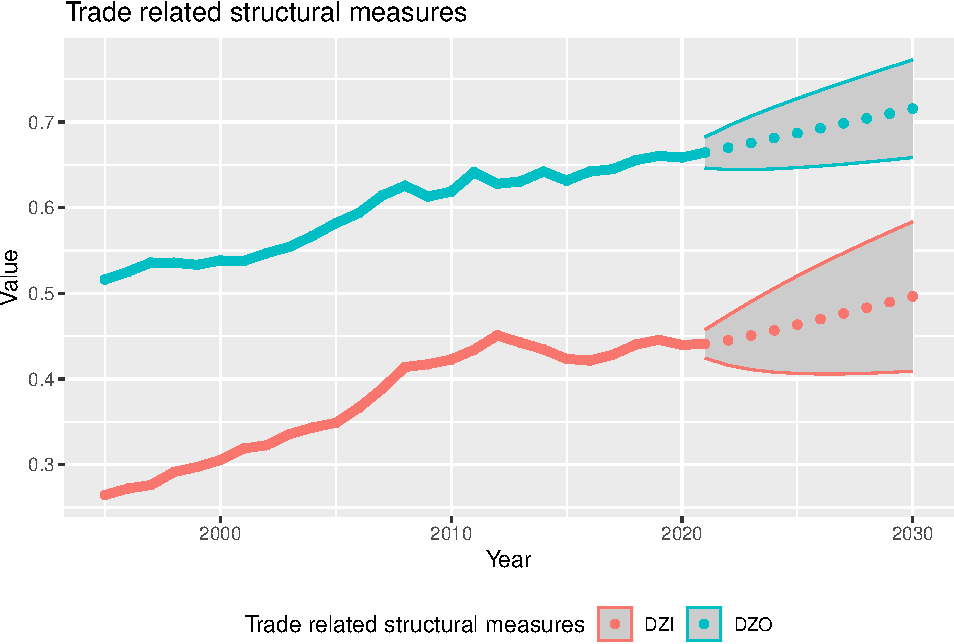
\includegraphics[width=0.33\linewidth]{netwp-1} }\subfloat[Resilience for random and systematic attacks\label{fig:netwp-2}]{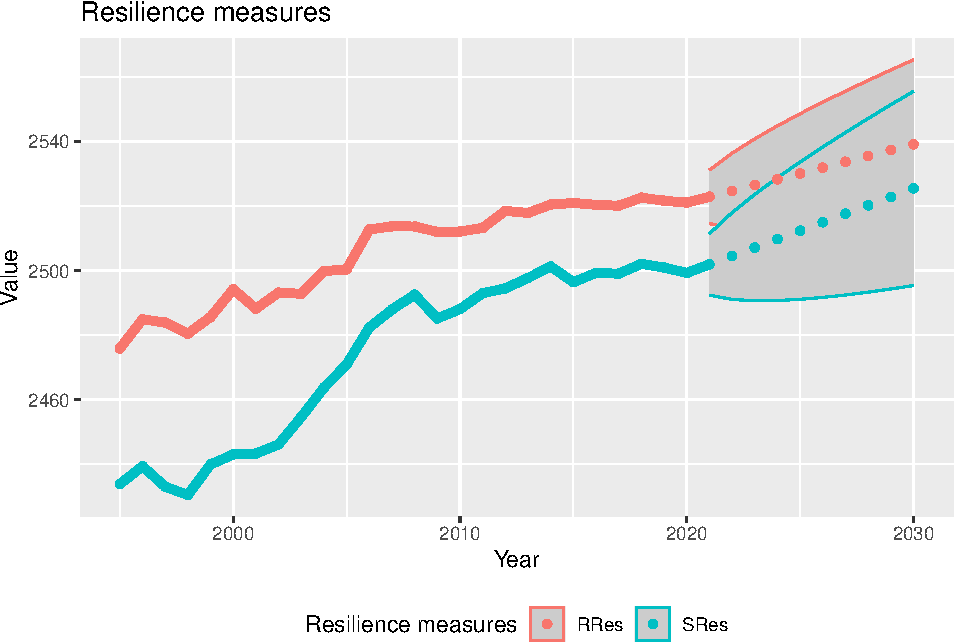
\includegraphics[width=0.33\linewidth]{netwp-2} }\subfloat[Average and global local efficiency and transitivity\label{fig:netwp-3}]{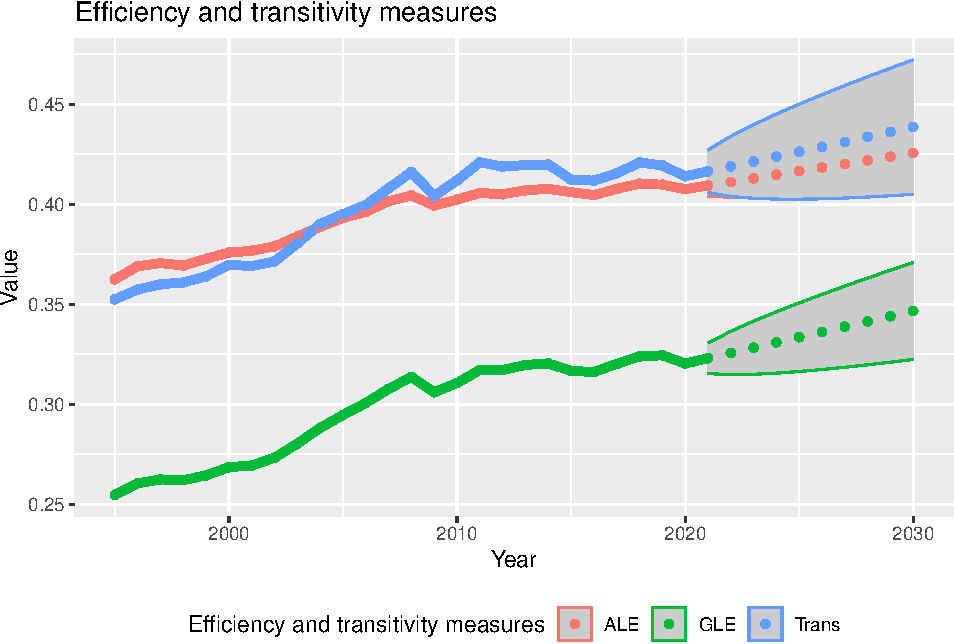
\includegraphics[width=0.33\linewidth]{netwp-3} }\newline\subfloat[PageRank centralizations and reach club cefficients\label{fig:netwp-4}]{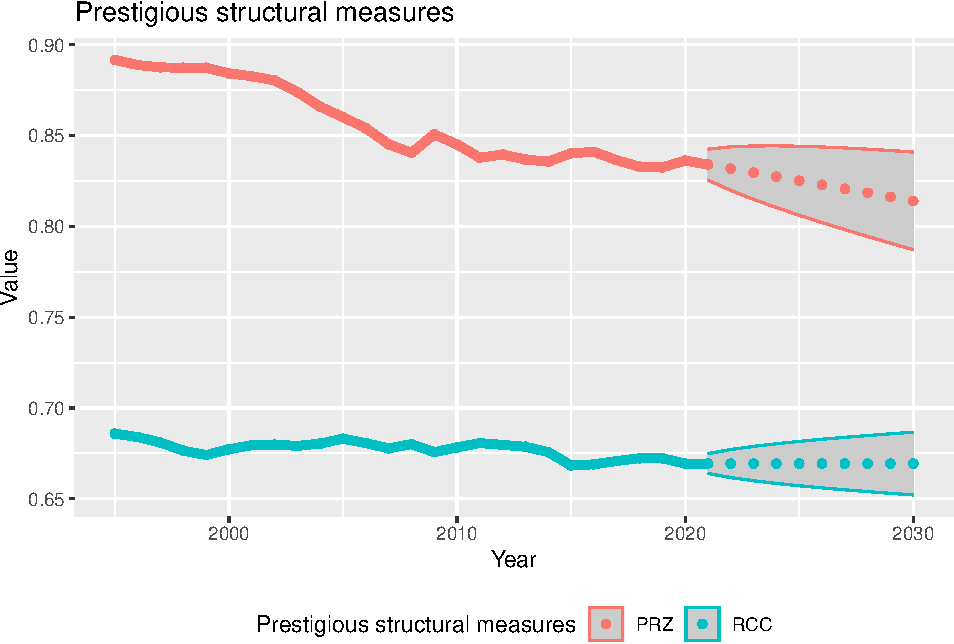
\includegraphics[width=0.33\linewidth]{netwp-4} }\subfloat[Modularity measures\label{fig:netwp-5}]{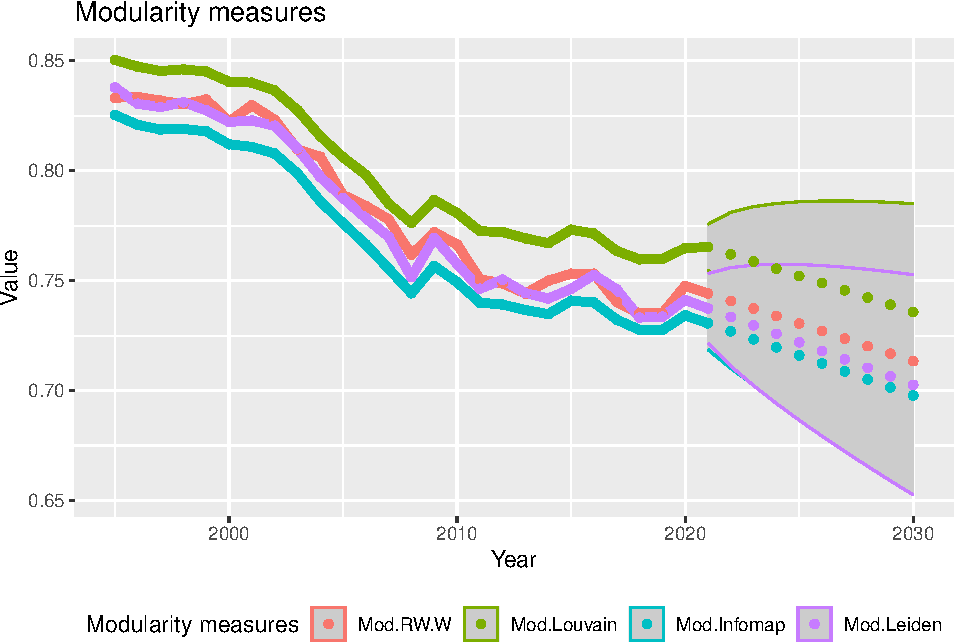
\includegraphics[width=0.33\linewidth]{netwp-5} }\subfloat[Average aggregated and multilayer path lengths\label{fig:netwp-6}]{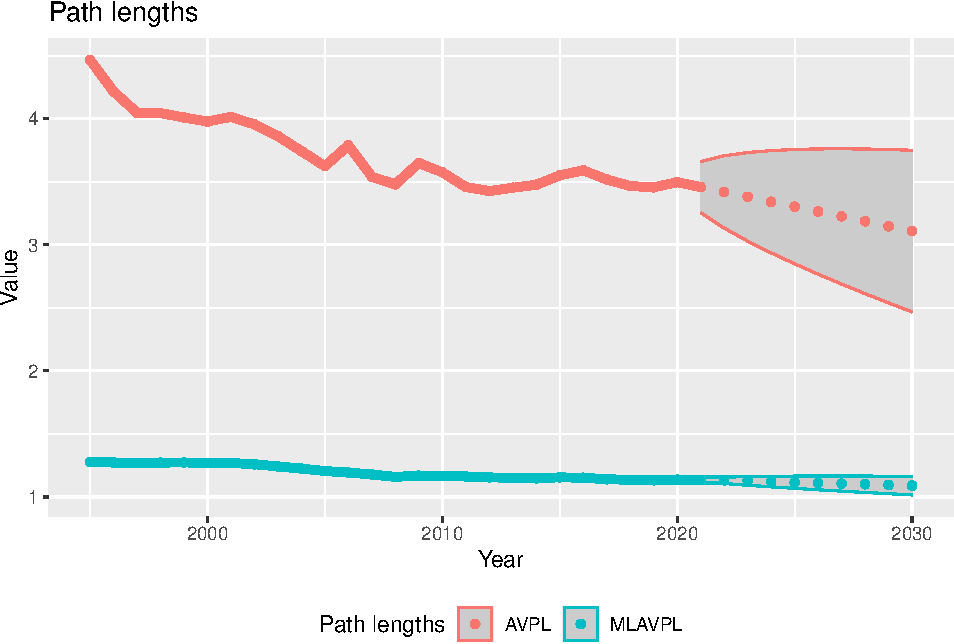
\includegraphics[width=0.33\linewidth]{netwp-6} }\newline\subfloat[Density, asymmetry and assortativity\label{fig:netwp-7}]{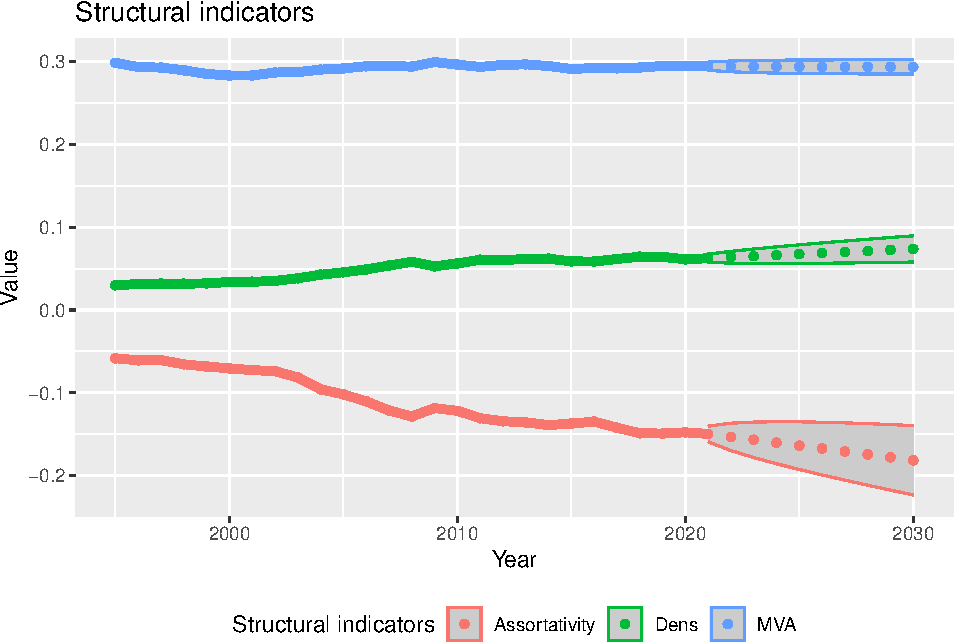
\includegraphics[width=0.33\linewidth]{netwp-7} }\subfloat[Betweennes and closeness centralizations\label{fig:netwp-8}]{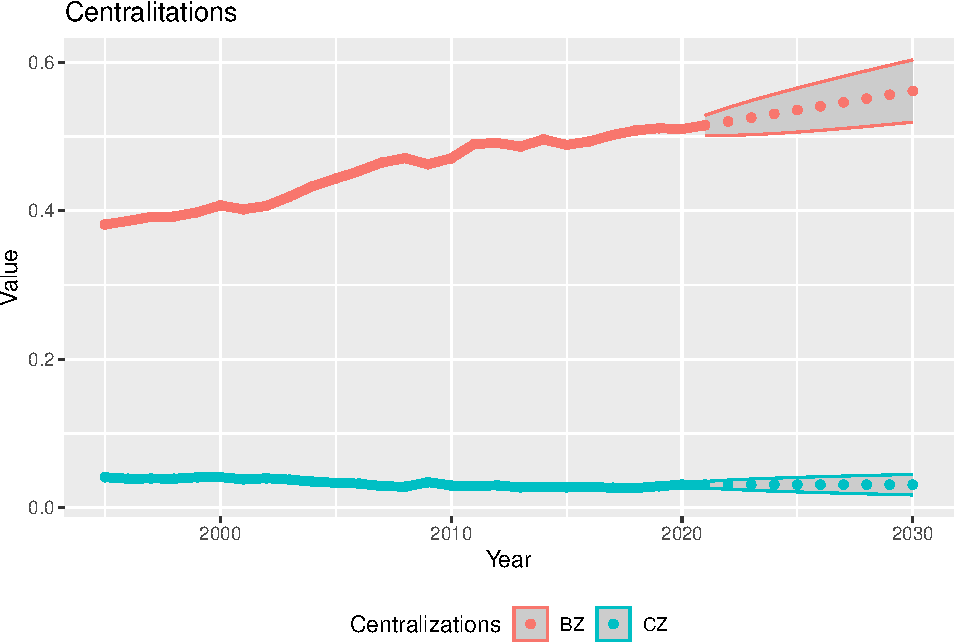
\includegraphics[width=0.33\linewidth]{netwp-8} }\subfloat[Average similarity values\label{fig:netwp-9}]{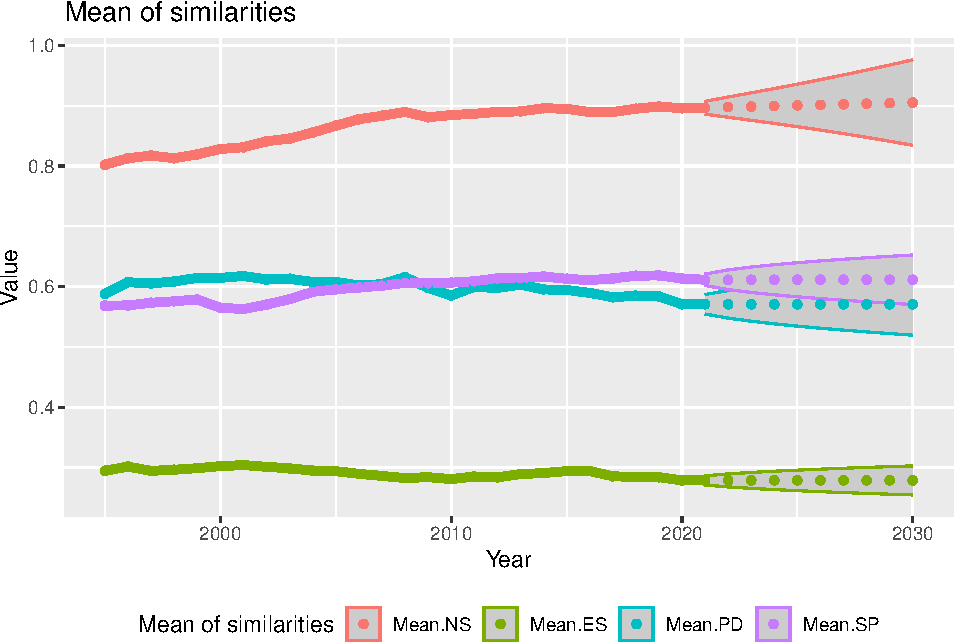
\includegraphics[width=0.33\linewidth]{netwp-9} }\newline

}

\caption{Network properties in time (forecast wth ARIMA, 95\% confidence interval)}\label{fig:netwp}
\end{figure}

Although the forecasts do not show what the impact of, for example,
Trump's protective tariffs or the prolongation of the Russia--Ukraine
conflict will be, causality analysis can show which structural
indicators move at the same time and which ones exhibit a time lag. The
causal relationship among the network properties are shown in Figure
\ref{fig:causnetwp}. Figure \ref{fig:causnetwp}(a-b) shows heatmaps and
biclusters of Granger (a) and instantaneous (b) causalities according to
the network features. The darker reddish cells in Figure
\ref{fig:causnetwp}(a) indicate longer lags; however, in the context of
instantaneous causality, there is no temporal lag, with only significant
cells depicted in dark red. In both causalities, two biclusters can be
identified, with only the first being significant for both rows and
columns. Figure \ref{fig:causnetwp}(c) illustrates a directed Granger
causality graph with a tree layout. On the basis of this arrangement and
clusterings, we create a block diagram, which is illustrated in Figure
\ref{fig:causnetwp}(e). Figure \ref{fig:causnetwp}(d) depicts an
undirected graph with instantaneous causality across properties. The
color of the nodes signifies the community identified by Leiden's
community-based modularity detection technique. The dimensions of the
nodes correspond to the \gls{dc} of each node, with dark red edges
representing members of the first bicluster (significant) and dark green
edges denoting members of the second bicluster (nonsignificant). In
accordance with Granger causality and the specified tree architecture,
three levels can be identified to minimize feedback, as shown in Figure
\ref{fig:causnetwp}(e).

\begin{figure}[H]

{\centering \subfloat[Granger causality (0= no sig., 1-5: year lags)\label{fig:causnetwp-1}]{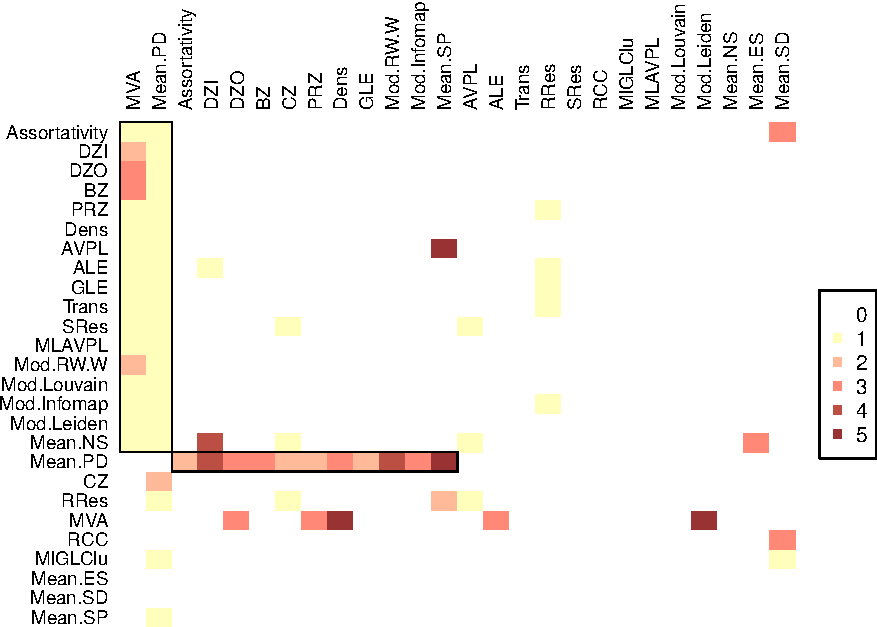
\includegraphics[width=0.48\linewidth]{causnetwp-1} }\subfloat[Instantaneous ($\circ$: no sig. \color{red!50!black}{$\bullet$}\color{black}: sig.) causality\label{fig:causnetwp-2}]{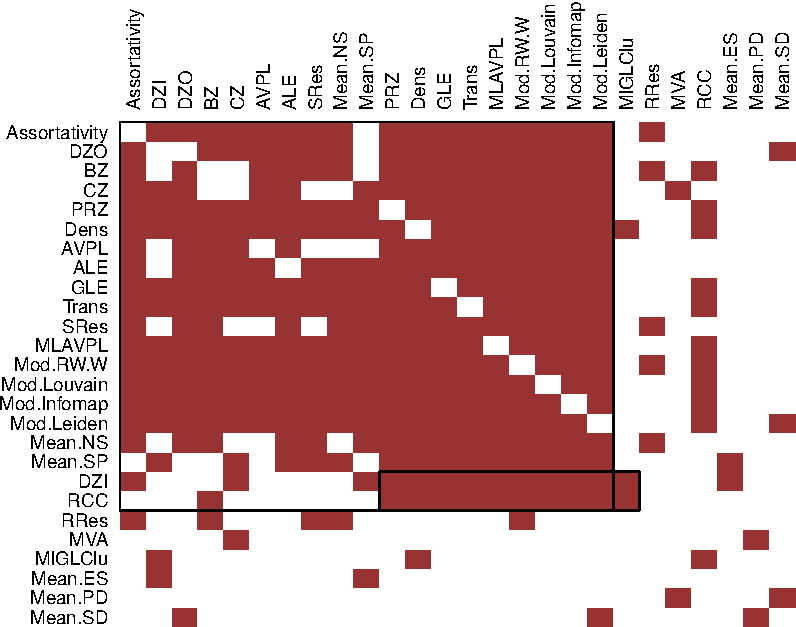
\includegraphics[width=0.48\linewidth]{causnetwp-2} }\newline\subfloat[Clustered Granger causality graph (\color{red!50!black}{$\longrightarrow $}\color{black}: pair of elements in bicluster 1)\label{fig:causnetwp-3}]{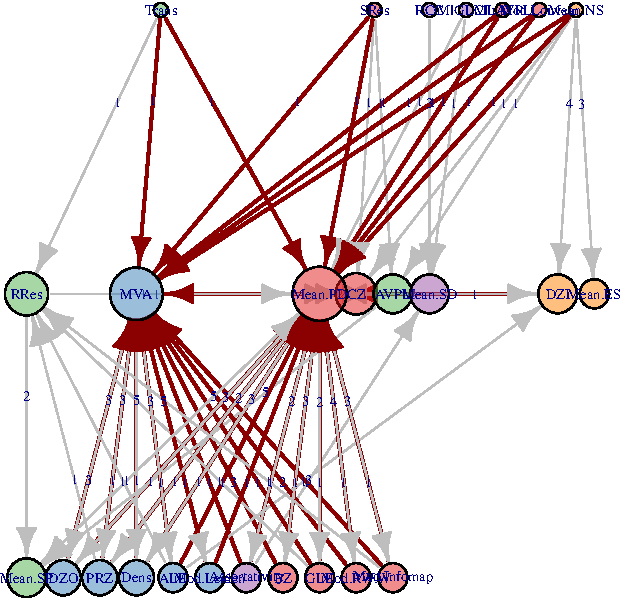
\includegraphics[width=0.48\linewidth]{causnetwp-3} }\subfloat[Clustered instantaneous causality graph (\color{green!50!black}{$\longrightarrow $}\color{black}: pair of elements in bicluster 2)\label{fig:causnetwp-4}]{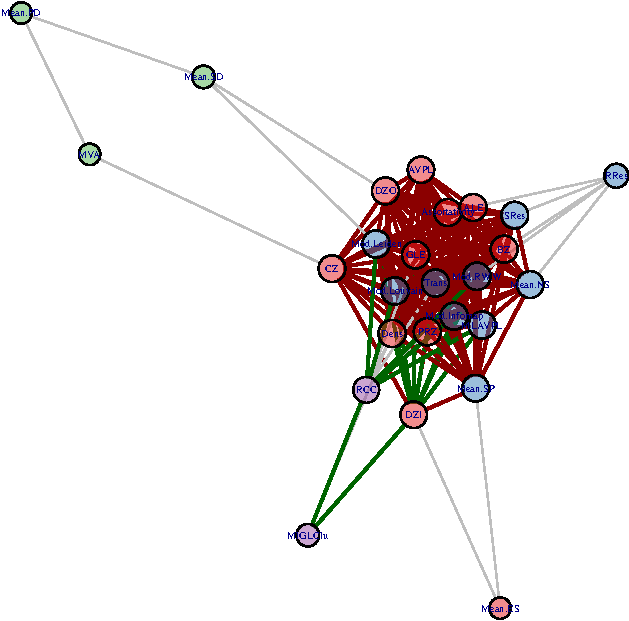
\includegraphics[width=0.48\linewidth]{causnetwp-4} }\newline\subfloat[The effect mechanism (average time lag of precedences)\label{fig:causnetwp-5}]{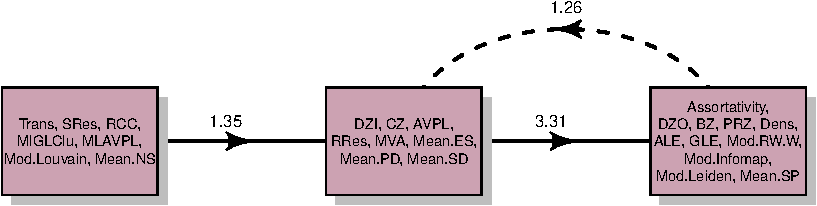
\includegraphics[width=0.48\linewidth]{causnetwp-5} }

}

\caption{Causalities between network properties with detailed methodological framework and indicator explanations}\label{fig:causnetwp}
\end{figure}

Figure \ref{fig:causnetwp} presents the comprehensive causality analysis
framework for multilayer trade network structural indicators from
1995-2020. To detemine the effect mechanism of each structural
indicator, we initially establish Granger and instantaneous causality
(see Figure \ref{fig:causnetwp}(a-b)). We cluster the structural
features by Leiden's modularity-based community detection (see Figure
\ref{fig:causnetwp}(c-d)) and by biclustering the relationships (see
Figure \ref{fig:causnetwp}(a-d)), and finally, we subsequently organize
the procedures to minimize the level of feedback among structural
elements (see Figure \ref{fig:causnetwp}(e)). Ultimately, we obtain a
mechanism graph illustrating both the comovements (i.e.,
\textasciitilde instantaneous correlations) and Granger causal linkages
(i.e.,\textasciitilde{} precedence) among structural components. The
weights in Figure \ref{fig:causnetwp}(e) inscribed on the arrows denote
the average duration of lags among the structural variables.

Specifically, Figure \ref{fig:causnetwp} (a) shows Granger causality
relationships with lag structure, where darker red cells indicate longer
temporal lags (0=no significance, 1-5=year lags) between structural
indicators. Key abbreviations: \gls{dzi}/\gls{dzo} - measuring trade
concentration, \gls{bz} - intermediary control, \gls{cz} - market
accessibility, \gls{prz} - influence concentration, \gls{avpl} - trade
route efficiency, \gls{ale}/\gls{gle} - regional/global trade
efficiency, Trans (Transitivity - clustering tendency),
\gls{rres}/\gls{sres} - network robustness, \gls{mva} - trade balance
inequalities, \gls{rcc} - elite country interactions, Mod.* (Various
modularity measures using different algorithms - community structure),
Mean.\gls{ns}/\gls{es}/\gls{pd}/\gls{sp} - cross-industry integration
patterns. Figure \ref{fig:causnetwp} (b) displays instantaneous
causality (simultaneous co-movements) where dark red dots indicate
significant relationships. Figures \ref{fig:causnetwp} (c) and (d)
present clustered causality graphs with community detection results,
where node colors represent different communities identified by Leiden's
modularity-based algorithm, and edge colors distinguish significant
(dark red) versus nonsignificant (dark green) biclusters. Figure
\ref{fig:causnetwp} (e) synthesizes the temporal mechanism into a
three-tier hierarchical structure: Tier 1 (robustness indicators:
\gls{trans}, \gls{sres}, \gls{rcc}, \gls{mlglclu}, \gls{mlavpl},
Mod.Louvain, Mean.NS) responds first to economic disruptions; Tier 2
(concentration indicators: \gls{dzi}, \gls{cz}, \gls{avpl}, \gls{rres},
\gls{mva}, Mean.\gls{es}/\gls{pd}/\gls{sp}) follows with 1.35-year
average lag; Tier 3 (structural integration indicators: Assortativity,
\gls{dzo}, \gls{bz}, \gls{prz}, \gls{dens}, \gls{ale}, \gls{gle},
Mod.RW.W (Modularity random walk (weighted)/Infomap/Leiden, Mean.SP)
responds last with 3.31-year average lag. Bidirectional arrows indicate
feedback effects with 1.26-year reverse lag between middle tiers.

\subsection{Industrial Causality Analysis and Temporal Pattern
Identification}\label{industrial-causality-analysis-and-temporal-pattern-identification}

Figure \ref{fig:top10sect} shows the main centrality values of the top
ten industries. The top 10 industries, in this case, are the 10 largest
industries with a given centrality. Figure \ref{fig:top10sect}(a) shows
the change in export volume, which is expressed in terms of \gls{sco}
centrality. The change in trade balance, which is the difference between
export and import volumes, and expressed in terms of centralities, is
\gls{sco}-\gls{sci} and shown in Figure \ref{fig:top10sect}(c).
Additional relative centrality values for the top 10 industries are
shown in Figure \ref{fig:top10sect}(b,d-g). The relative centrality for
each industry is calculated by dividing the industry centrality value by
that of all industries. To validate the results we also calculated the
relative sectorial added values (see Figure \ref{fig:top10sect}(h)).

\begin{figure}[H]

{\centering \subfloat[Out-strength centralities (total exports)\label{fig:top10sect-1}]{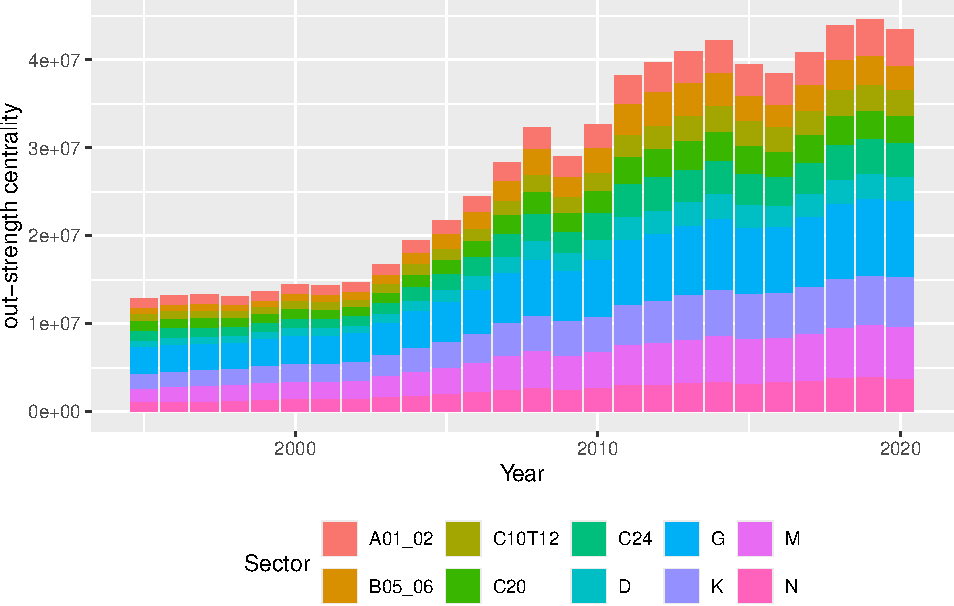
\includegraphics[width=0.33\linewidth]{top10sect-1} }\subfloat[Relative PageRank centalities\label{fig:top10sect-2}]{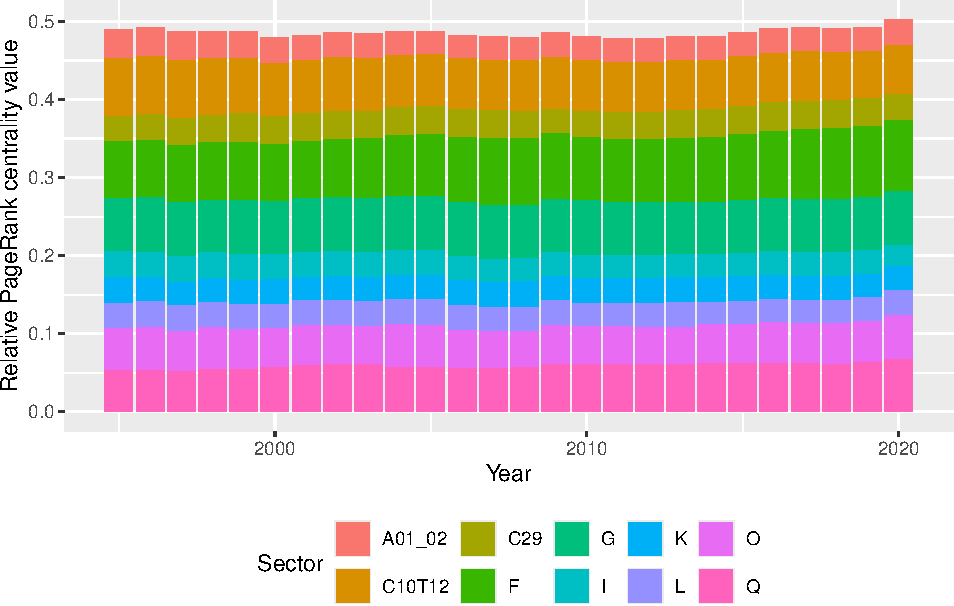
\includegraphics[width=0.33\linewidth]{top10sect-2} }\subfloat[Difference out- and in-stregth centralities\label{fig:top10sect-3}]{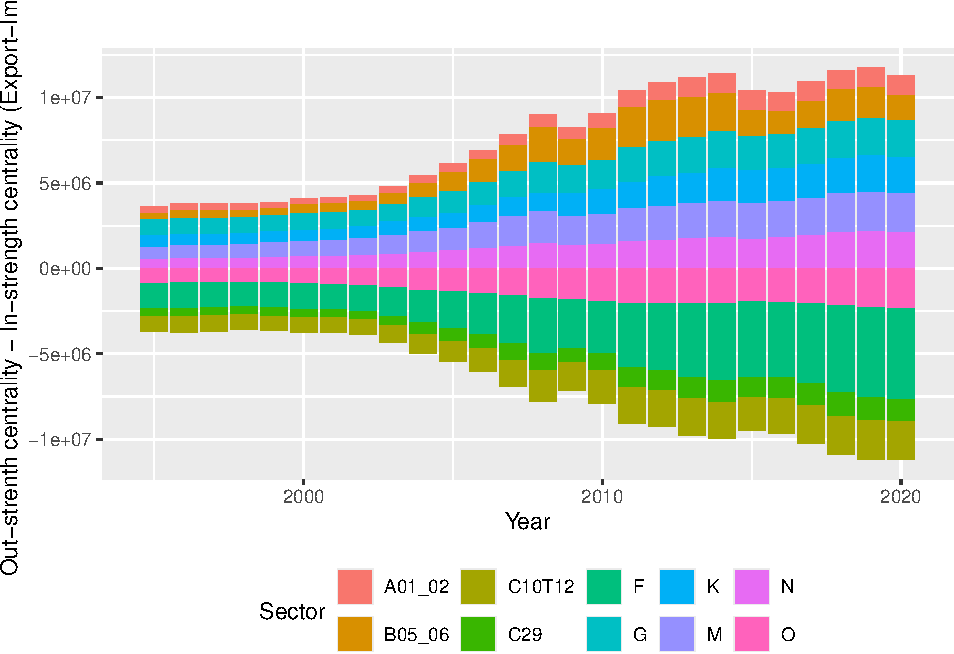
\includegraphics[width=0.33\linewidth]{top10sect-3} }\newline\subfloat[Hub centrality\label{fig:top10sect-4}]{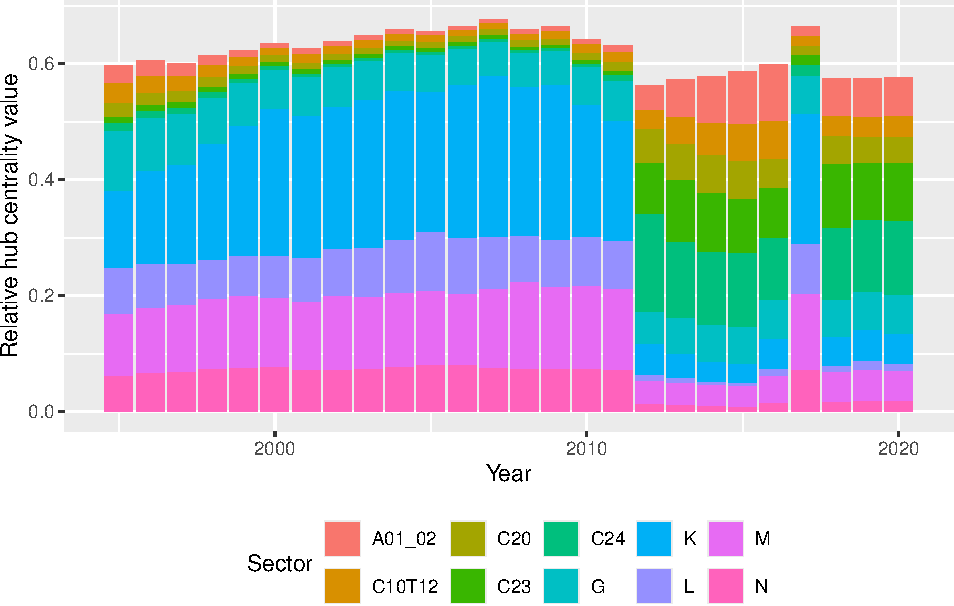
\includegraphics[width=0.33\linewidth]{top10sect-4} }\subfloat[Authority centrality\label{fig:top10sect-5}]{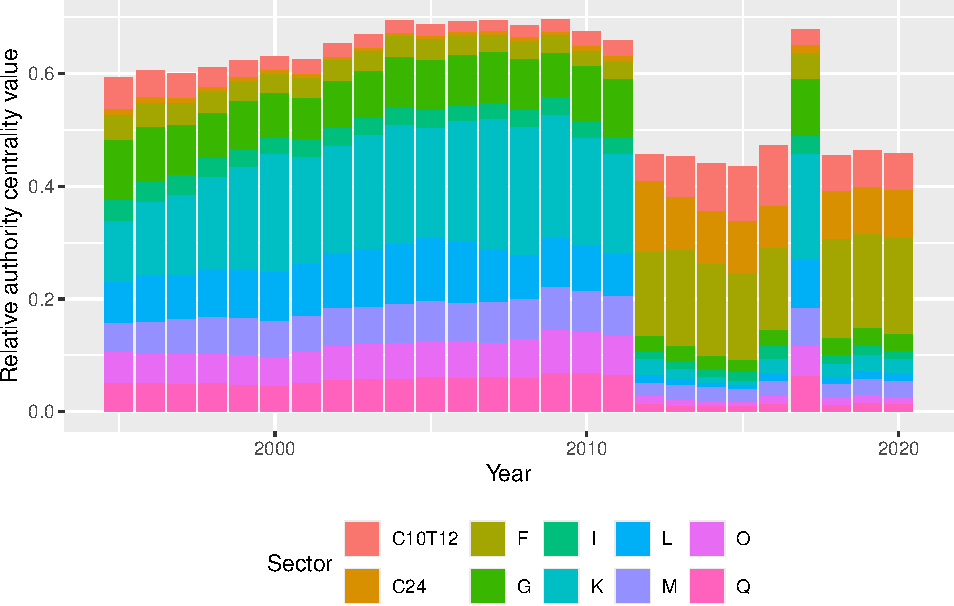
\includegraphics[width=0.33\linewidth]{top10sect-5} }\subfloat[Betweenness centrality\label{fig:top10sect-6}]{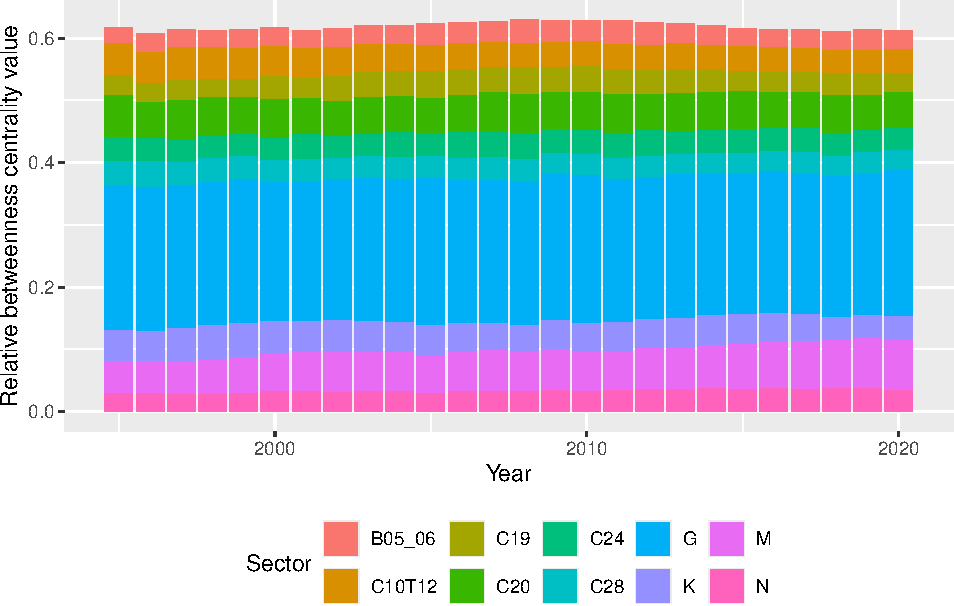
\includegraphics[width=0.33\linewidth]{top10sect-6} }\newline\subfloat[Eigenvector centrality\label{fig:top10sect-7}]{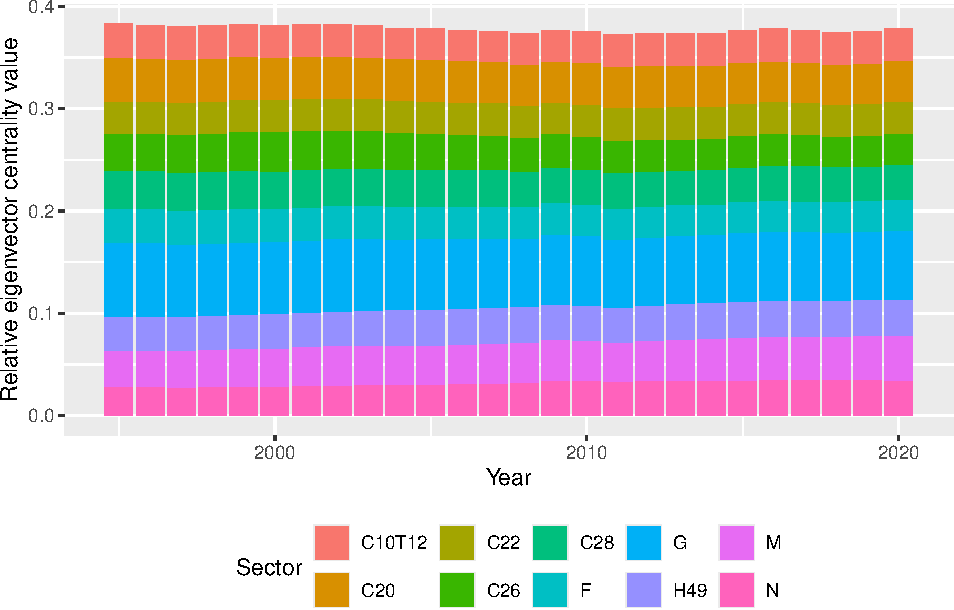
\includegraphics[width=0.33\linewidth]{top10sect-7} }\subfloat[Relative added values (VAs)\label{fig:top10sect-8}]{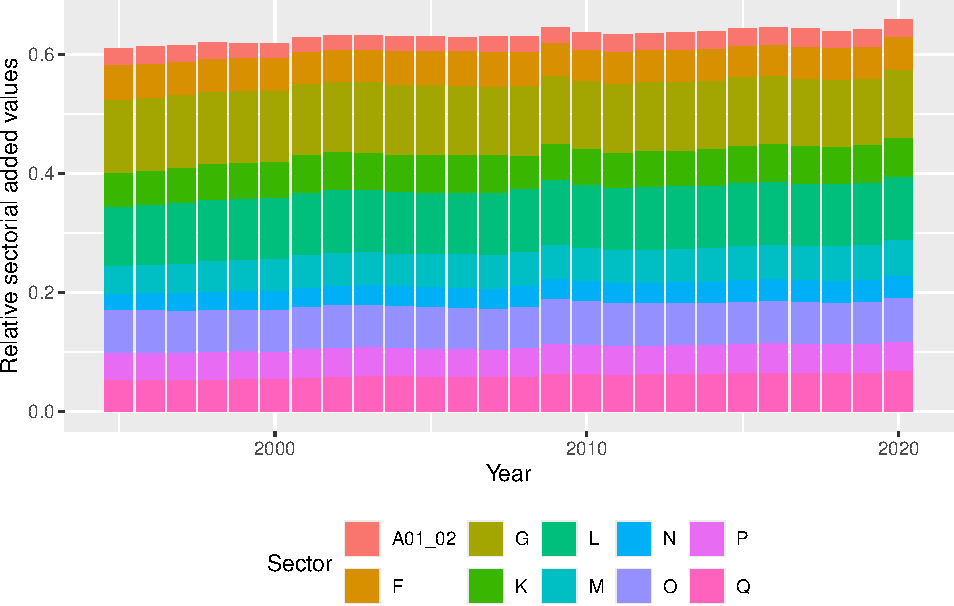
\includegraphics[width=0.33\linewidth]{top10sect-8} }

}

\caption{Centrality values of the top 10 industries}\label{fig:top10sect}
\end{figure}

To determine the typical industrial trends, we cluster the node-level
indicators by employing the \gls{gnda} approach. Figure
\ref{fig:sectpnda} shows the temporal patterns of the node-level
indicators aggregated by industry. The employed \gls{gnda} identifies
the number of temporal characteristics (i.e., cluster centers). The
temporal patterns of cluster centers shows how the aggregate
characteristics of the industries in a given group have changed on
average. All industries that belong to such an aggregate (latent)
characteristic are listed in the legend. To ensure that the forecasts
the Bayesian version of ARIMA models are also shown in Figure
\ref{fig:bayessectpnda} in the Appendix. The results of the classical
and Bayesian approaches differ only minimally.

We analyze six indicators. First, \gls{dco} illustrates the temporal
progression of the quantity of export partners, indicating the average
number of buyers a country possesses within an industry (see Figure
\ref{fig:sectpnda}(a)). The second indicator (see Figure
\ref{fig:sectpnda}(b)) examined is homophily, which shows what
percentages of countries' import and export relationships in a given
industry originate from that industry. This indicator characterizes the
structure of the industry. The development of homophily over time can
show how much the industry is integrated into the international market.
If the indicator increases, then it may indicate that the trade
relationships between the actors in the given industry are
strengthening, while if it decreases, then the opposite situation may
occur. The third indicator analyzed is modularity (see Figure
\ref{fig:sectpnda}(c)). Modularity demonstrates the significant
separation of clusters, or modules (communities), inside a network
structure. Assessing modularity helps determine the degree to which
specific countries create communities within particular industries. The
temporal variation in modularity enables the observation of how linkages
among industry actors have evolved into communities. Figures
\ref{fig:sectpnda} (e-g) illustrate the time evolution of most important
industrial centrality indicators, such as \gls{ec} (e), \gls{prc} (f),
and \gls{bc} (g). While \gls{ec} and \gls{prc} demonstrate the role of
industries inside the network, \gls{bc} illustrates their intermediary
function. To validate the change in centrality values the added values
are also calculated (h).

\begin{figure}[H]

{\centering \subfloat[Outdegree centrality\label{fig:sectpnda-1}]{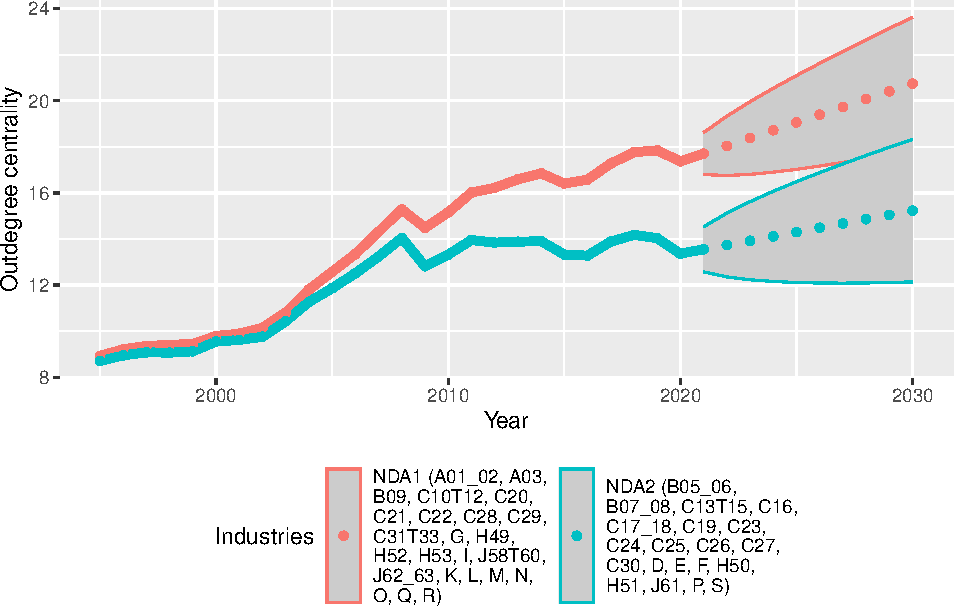
\includegraphics[width=0.33\linewidth]{sectpnda-1} }\subfloat[Homophily\label{fig:sectpnda-2}]{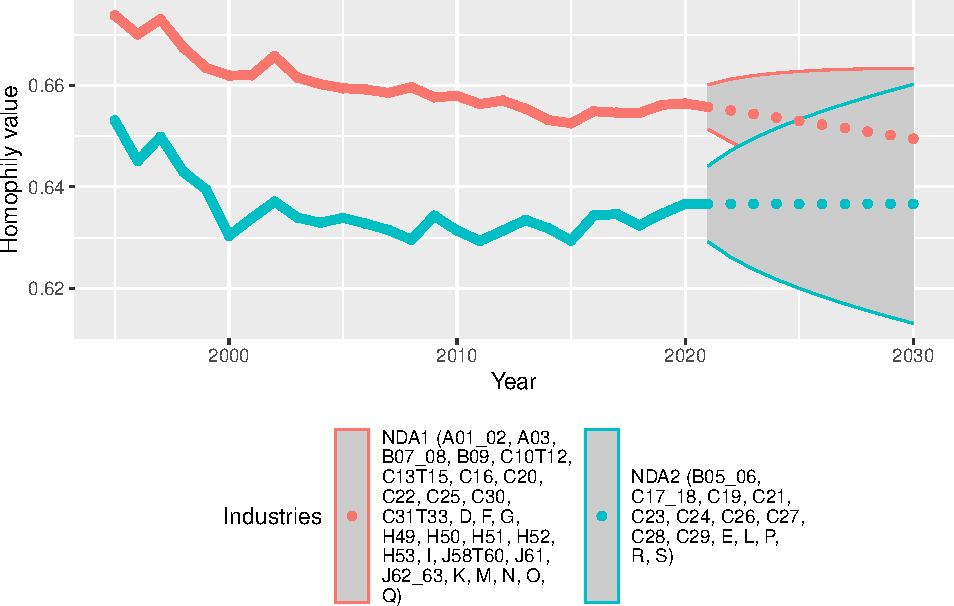
\includegraphics[width=0.33\linewidth]{sectpnda-2} }\subfloat[Leiden's modularity\label{fig:sectpnda-3}]{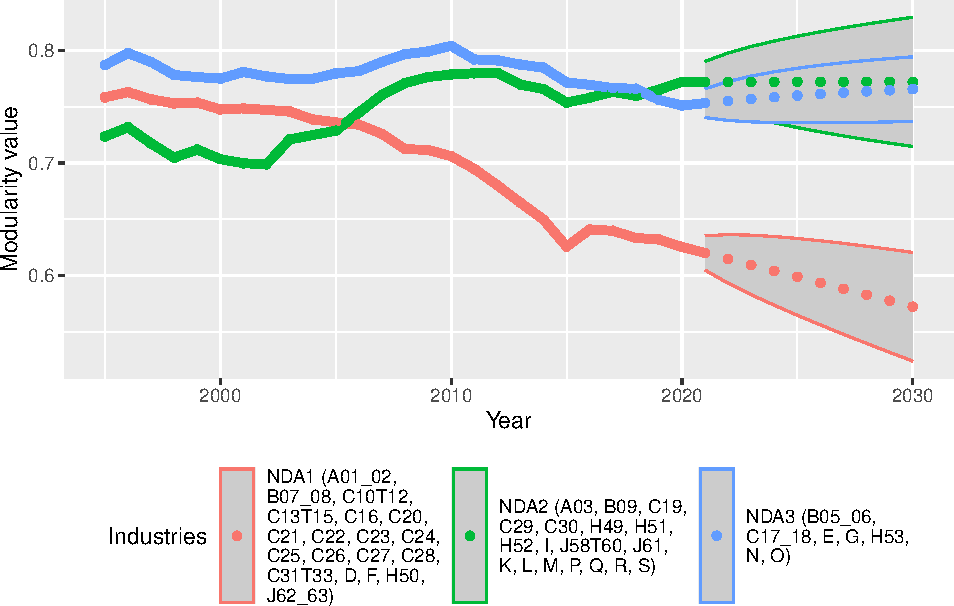
\includegraphics[width=0.33\linewidth]{sectpnda-3} }\newline\subfloat[Eigenvector centrality\label{fig:sectpnda-4}]{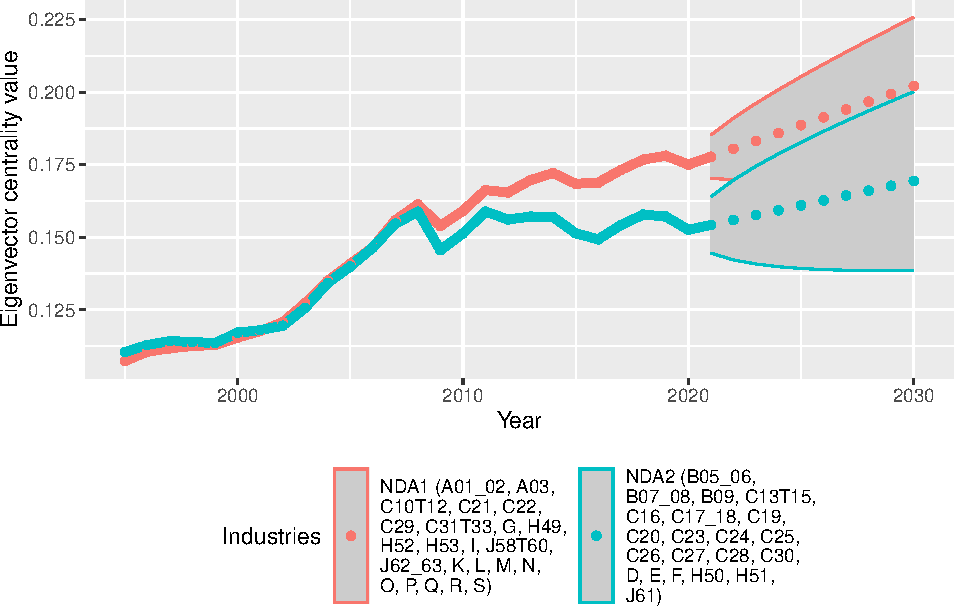
\includegraphics[width=0.33\linewidth]{sectpnda-4} }\subfloat[PageRank centrality\label{fig:sectpnda-5}]{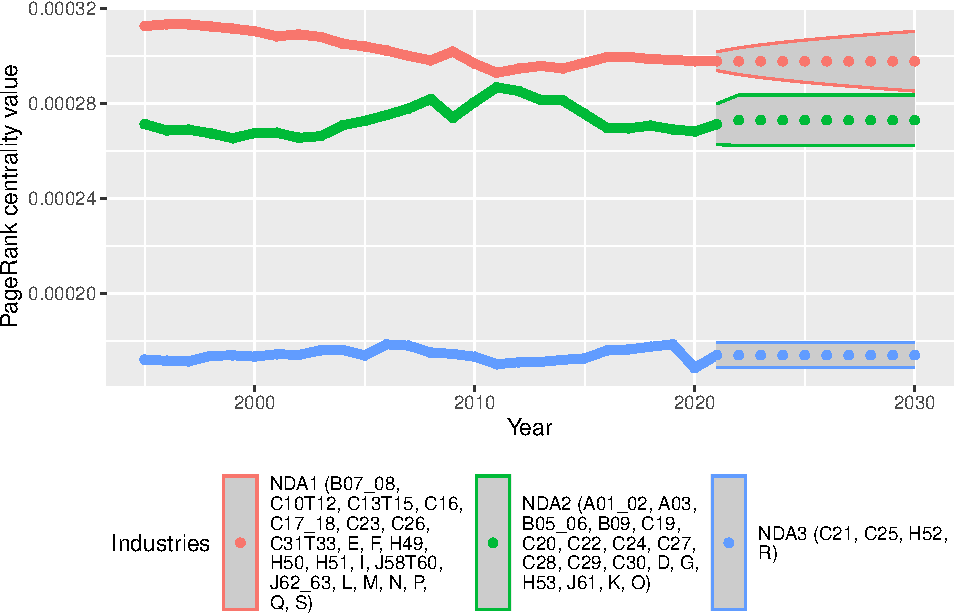
\includegraphics[width=0.33\linewidth]{sectpnda-5} }\subfloat[Betweenness centrality\label{fig:sectpnda-6}]{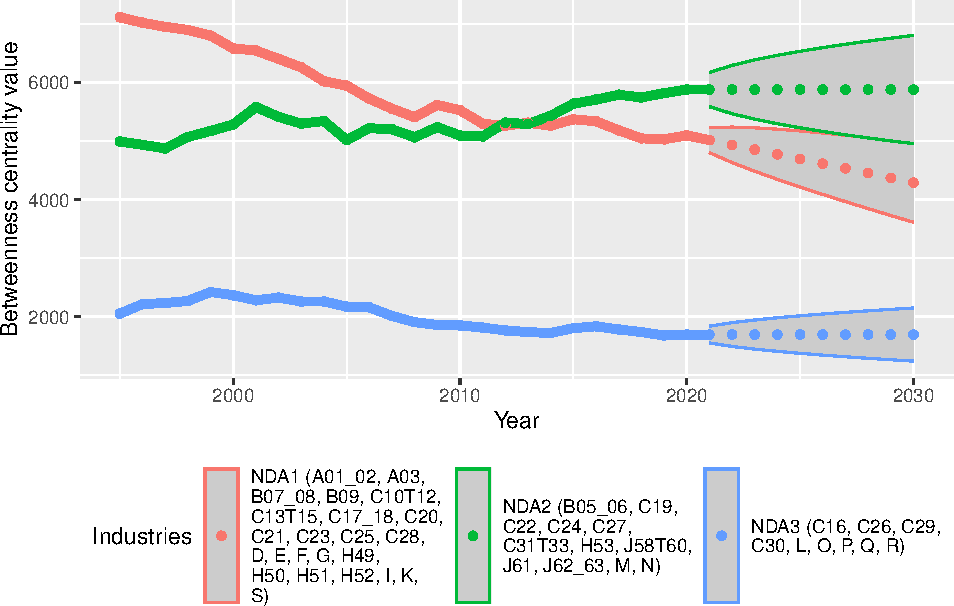
\includegraphics[width=0.33\linewidth]{sectpnda-6} }\newline\subfloat[Added values (VAs)\label{fig:sectpnda-7}]{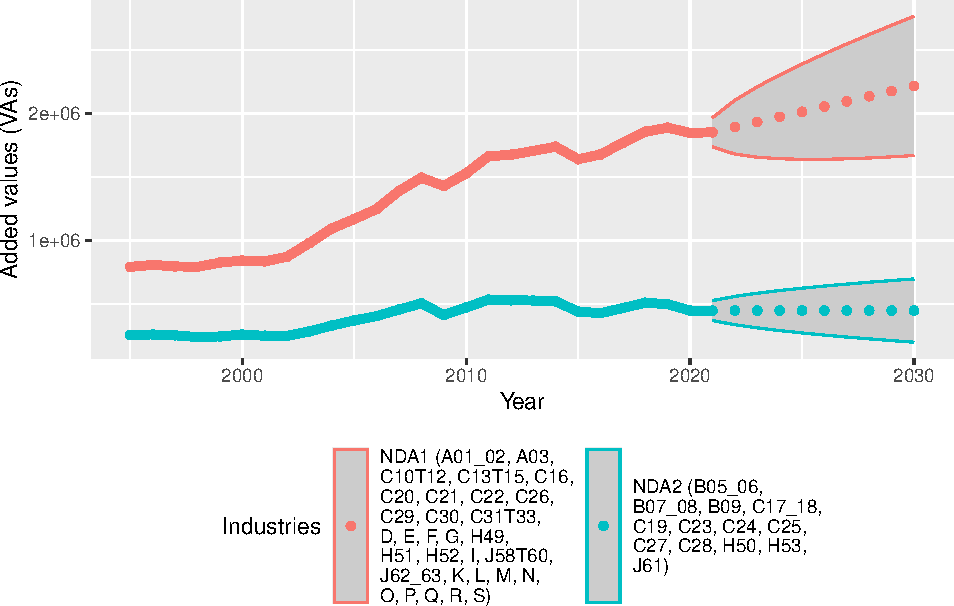
\includegraphics[width=0.33\linewidth]{sectpnda-7} }

}

\caption{Average clustered industrial node-level properties}\label{fig:sectpnda}
\end{figure}

The final results of the causality analysis are shown in Figure
\ref{fig:caussect}. This calculation follows the steps of causality
analysis on network-level indicators; see Figure \ref{fig:causnetwp}.
First, the Granger and instantaneous causalities are calculated.
Causality graphs are specified and aligned as a tree layout. Each level
of trees is grouped into a block, and the average time lag between the
pair of elements from a two distinct blocks is calculated.

\begin{figure}[H]

{\centering \subfloat[Outdegree centrality, homophily, modularity\label{fig:caussect-1}]{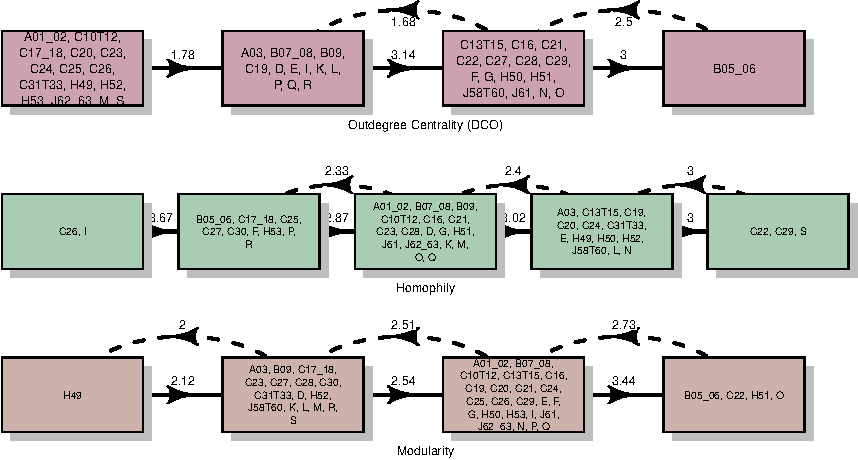
\includegraphics[width=0.48\linewidth]{caussect-1} }\subfloat[Eigenvector centrality, PageRank Centrality, Betweenness Centrality\label{fig:caussect-2}]{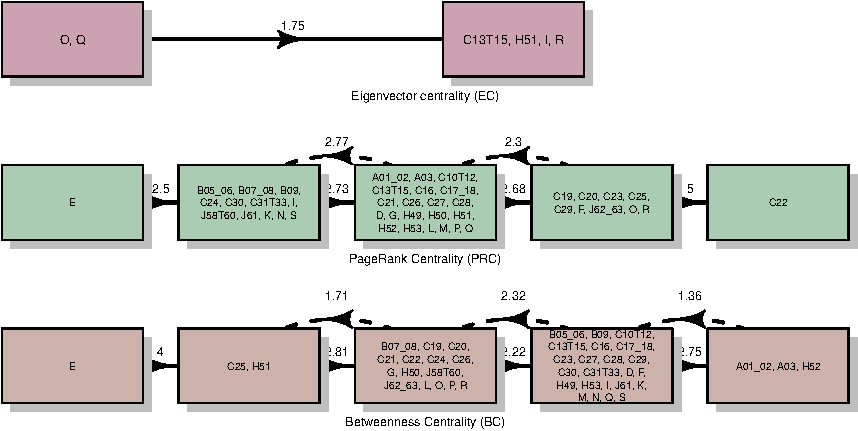
\includegraphics[width=0.48\linewidth]{caussect-2} }

}

\caption{Industrial effect mechanisms based on causality and cluster analysis with economic interpretation of sectoral groupings}\label{fig:caussect}
\end{figure}

\subsection{Country-Level Analysis}\label{country-level-analysis}

Figure \ref{fig:top10ctry} shows the top ten countries with the greatest
centrality values. The \gls{sco} in Figure \ref{fig:top10ctry}(a)
actually shows the volume of exports considering the ten largest
exporters, whereas Figure \ref{fig:top10ctry}(c) shows the trade balance
\gls{sco}-\gls{sci}=export-import in time. Figure \ref{fig:top10ctry}(b,
d-g) shows the ten most important countries with the largest relative
PageRank, hub, authority, betweenness and eigenvector centrality values,
where the relative centrality value of a given country is calculated by
dividing the summed centrality values of all industries of that country
by the sum of the centrality values of all industries of all countries.
In this way, the sum of the relative centrality values of the top ten
countries with the greatest values indicate their role compared to that
of all other countries. The change in values over time gives the change
in the relative position of the top ten countries. To control the
changes in centralities we calculate the changes in \glspl{fd} (see
Figure \ref{fig:top10ctry}(h)).

\begin{figure}[H]

{\centering \subfloat[Out-strength centralities (total exports)\label{fig:top10ctry-1}]{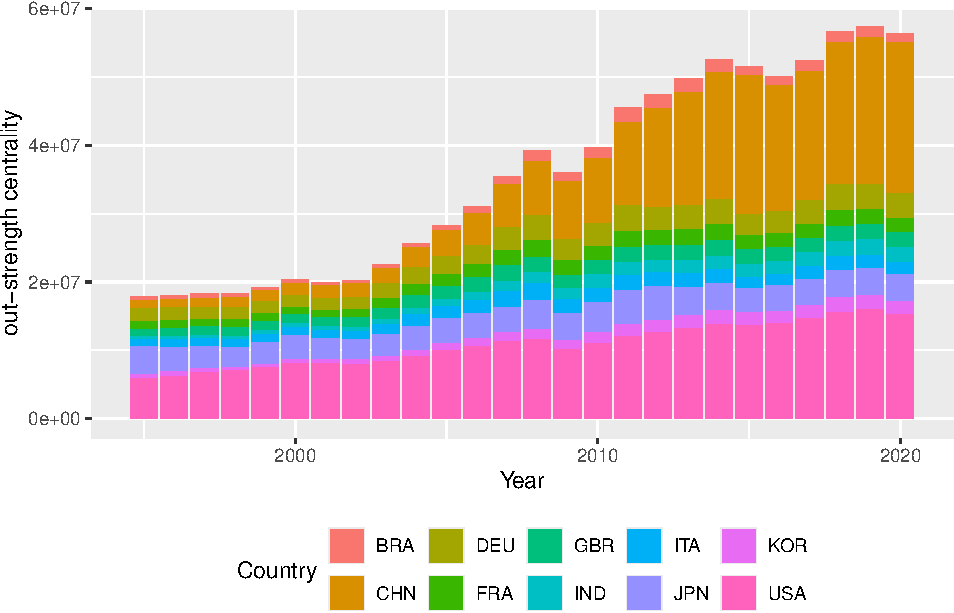
\includegraphics[width=0.33\linewidth]{top10ctry-1} }\subfloat[Relative PageRank centalities\label{fig:top10ctry-2}]{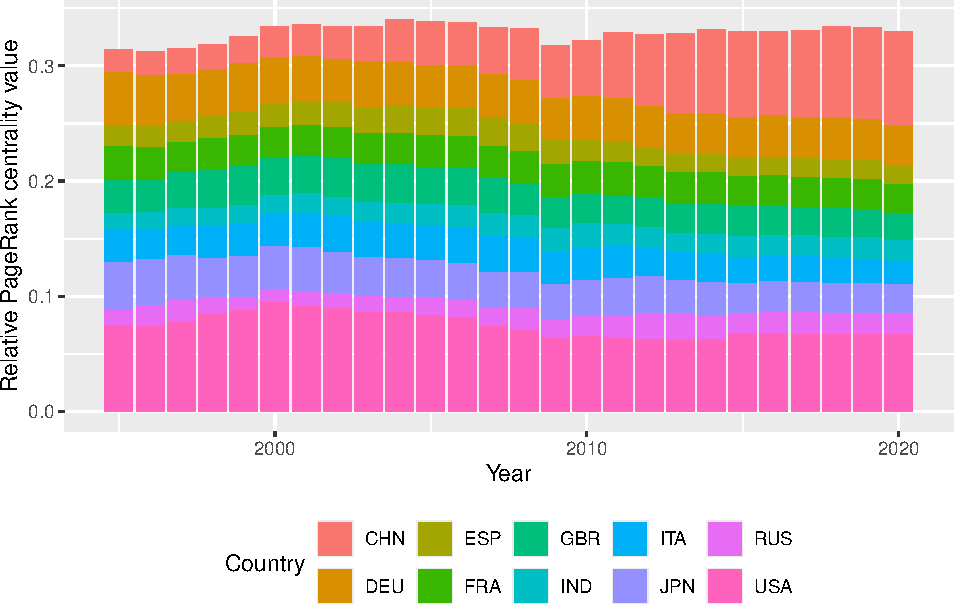
\includegraphics[width=0.33\linewidth]{top10ctry-2} }\subfloat[Difference out- and in-stregth centralities\label{fig:top10ctry-3}]{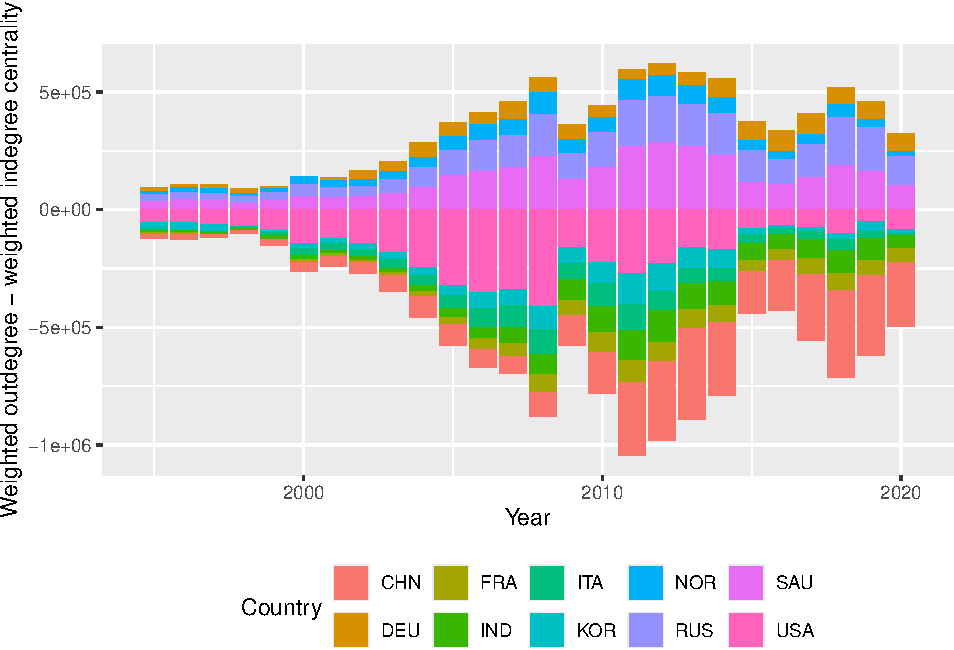
\includegraphics[width=0.33\linewidth]{top10ctry-3} }\newline\subfloat[Hub centrality\label{fig:top10ctry-4}]{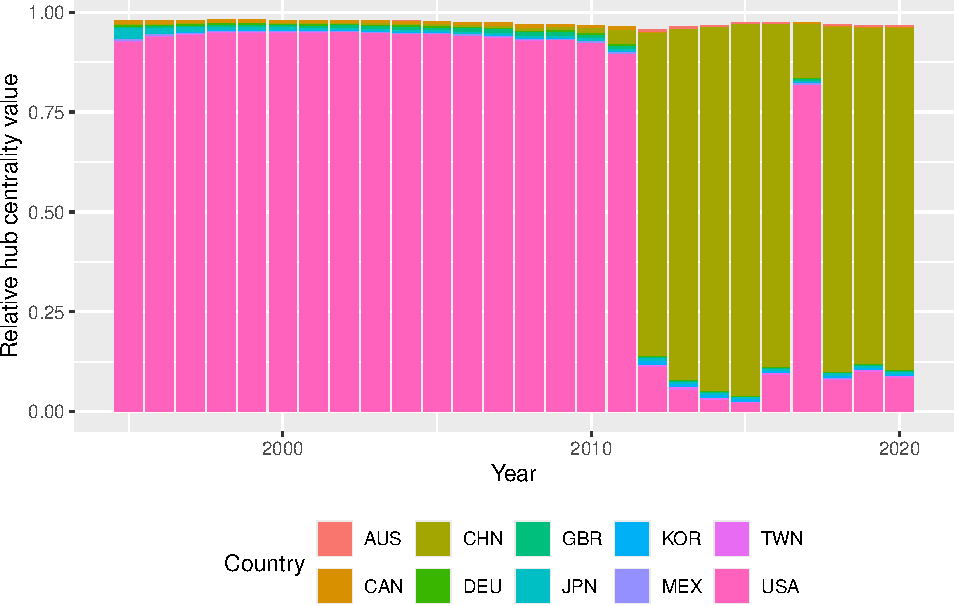
\includegraphics[width=0.33\linewidth]{top10ctry-4} }\subfloat[Authority centrality\label{fig:top10ctry-5}]{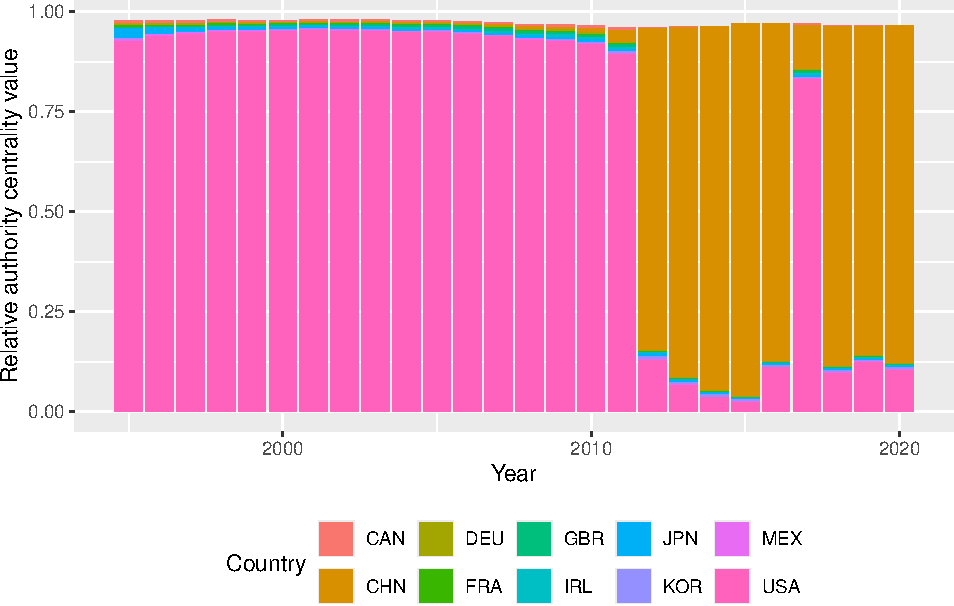
\includegraphics[width=0.33\linewidth]{top10ctry-5} }\subfloat[Betweenness centrality\label{fig:top10ctry-6}]{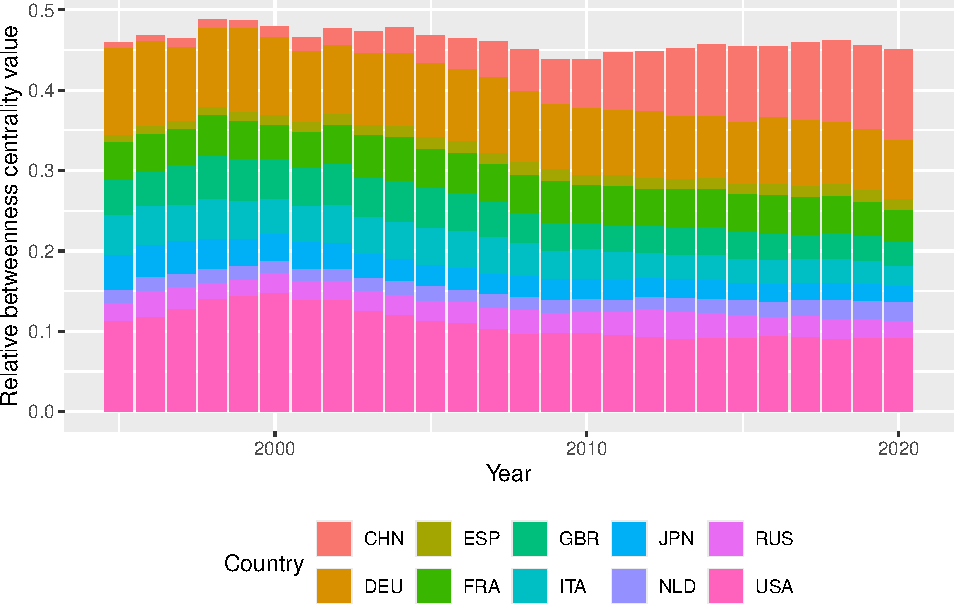
\includegraphics[width=0.33\linewidth]{top10ctry-6} }\newline\subfloat[Eigenvector centrality\label{fig:top10ctry-7}]{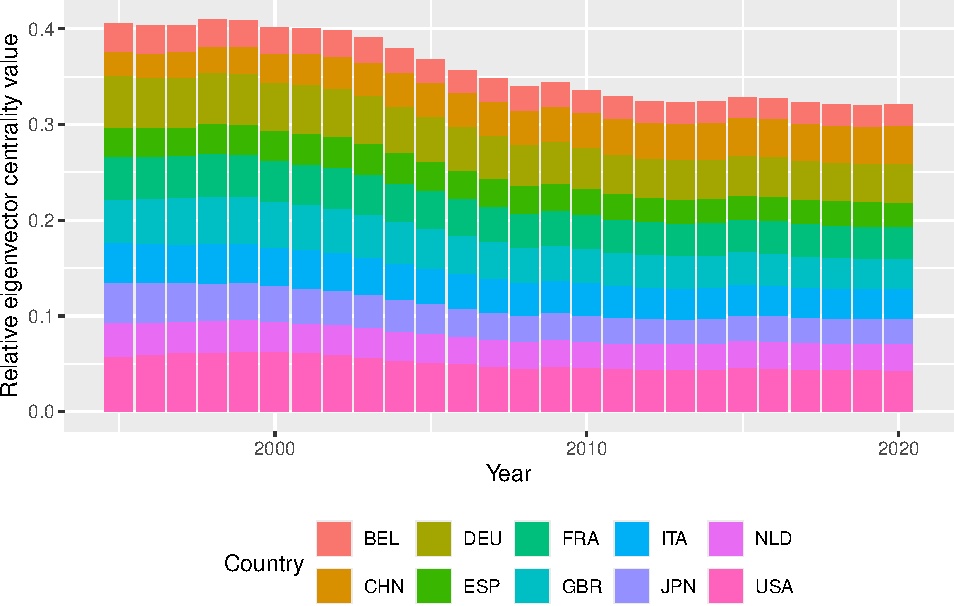
\includegraphics[width=0.33\linewidth]{top10ctry-7} }\subfloat[Relative final demands (FDs)\label{fig:top10ctry-8}]{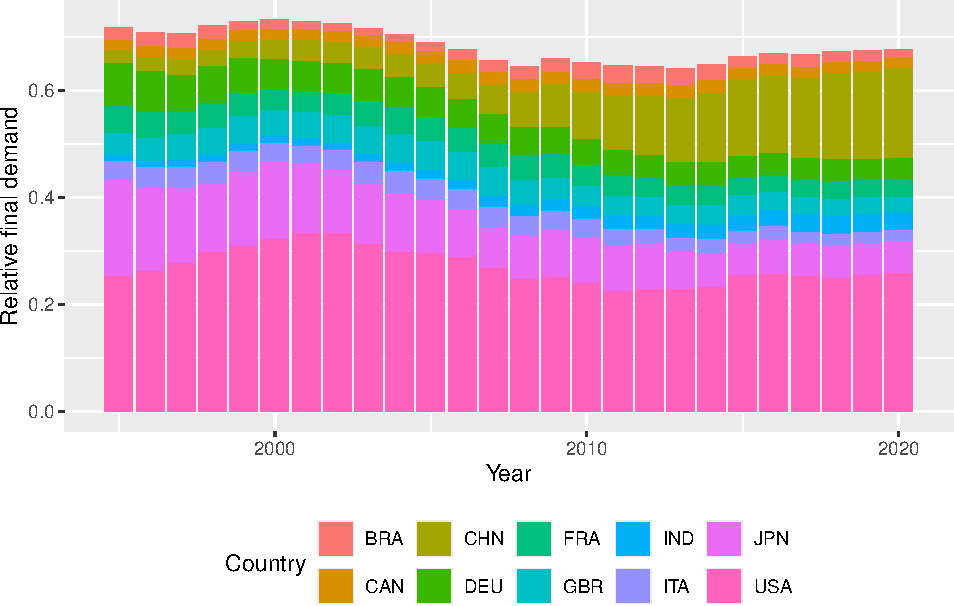
\includegraphics[width=0.33\linewidth]{top10ctry-8} }

}

\caption{Centrality values of the top 10 countries}\label{fig:top10ctry}
\end{figure}

Figure \ref{fig:ctryaggr} shows the impact mechanism of changes in all
trade activities (import+export with \gls{sc}) measured. The map shows
OECD countries. The size of the nodes is proportional to the total trade
activity (imports + exports), which is measured via strength centrality.
The colors of the nodes indicate the causal group into which each
country falls. The first causal relationship is for countries whose
trade changes first. The last causal relationship is for countries whose
trade changes last. By biclustering the causal relations, one
significant group of relationships can be identified, which are
indicated by the colors of the arrows.

\begin{figure}[H]

{\centering \subfloat[Clustered Granger causality graph (\color{red!50!black}{$\longrightarrow $}\color{black}: bicluster 1 (significant), \color{green!50!black}{$\longrightarrow $}\color{black}: bicluster 2 (non significant))\label{fig:ctryaggr-1}]{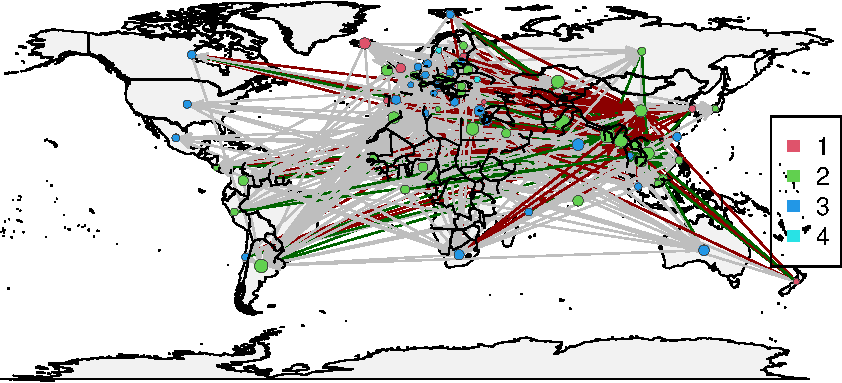
\includegraphics[width=0.99\linewidth]{ctryaggr-1} }\newline\subfloat[Effect mechanism\label{fig:ctryaggr-2}]{
\includegraphics[width=0.99\linewidth]{ctryaggr-2} }\newline

}

\caption{Country-level causality effect mechanism of strength centrality (total trade volume) with geographic and economic development patterns}\label{fig:ctryaggr}
\end{figure}

Figure \ref{fig:ctryaggr} maps the temporal propagation of trade volume,
which changes across 77 countries from 1995-2020, revealing systematic
patterns in how global trade disruptions cascade through different
national economies. Figure \ref{fig:ctryaggr} (a) presents the clustered
Granger causality network where nodes represent country size
proportionally to total trade activity (imports + exports measured by
strength centrality), and node colors indicate causal group membership
based on response timing. Dark red arrows represent significant causal
relationships (bicluster 1) where changes in one country's trade volume
predict changes in another with specific time lags, while light green
arrows show nonsignificant relationships (bicluster 2). Figure
\ref{fig:ctryaggr} (b) synthesizes the effect mechanism into four
hierarchical tiers with distinct economic characteristics. Figure
\ref{fig:ctryaggr} shows that the change in trade occurs simultaneously
in most countries. Such changes can be divided into four consecutive
causal groups in time. Trade changes first appear in Côte d'Ivoire,
Estonia, United Kingdom, Hong Kong, China, Croatia, Iceland, Korea, New
Zealand, Portugal, Turkey. Afterward, at average, in 2.25 years, the
larger set of trade countries is Argentina, Belgium, Bangladesh,
Bulgaria, Belarus, Brunei Darussalam, Switzerland, China (People's
Republic of), Cameroon, Colombia, Costa Rica, Czechia, Egypt, Finland,
Indonesia, Ireland, Israel, Japan, Kazakhstan, Cambodia, Lao (People's
Democratic Republic), Lithuania, Morocco, Malta, Myanmar, Malaysia,
Nigeria, Pakistan, Peru, Philippines, Romania, Russian Federation, Saudi
Arabia, Senegal, Slovakia, Vietnam, rest of the world. A change in a
larger group of countries can also be observed, on average, 2.94 years
later, such as Australia, Austria, Brazil, Canada, Chile, Cyprus,
Germany, Denmark, Spain, France, Greece, Hungary, India, Italy, Jordan,
Luxembourg, Latvia, Mexico, Netherlands, Norway, Poland, Singapore,
Slovenia, Thailand, Tunisia, Chinese Taipei, United States, South
Africa. A backlash can also be observed between the two middle groups
with an average delay of 1.92 years. The last group includes a total of
2 countries, namely Sweden, Ukraine, which are those countries where
export/import changes in trade appear the latest in the considered
period.

\section{Discussion}\label{discussion}

\subsection{Structural Changes in the Trade
Network}\label{structural-changes-in-the-trade-network}

Concentration and market power. The steady rise of importer and exporter
centralization and of intermediation power (degree and betweenness
centralizations; PageRank centralization; ``rich-club'' intensity)
signals a persistent concentration of global trade in a relatively small
set of hub economies. Economically, this implies growing bargaining
power for core countries and lead firms, stronger price-setting capacity
along \glspl{gvc}, and a greater potential for policy shocks in a few
jurisdictions to transmit widely. The timing is consistent with
welldocumented structural drivers: the post-1995 offshoring boom, the
2001 \gls{wto} accession of China, and the scaling of platform-type
supply chains. Nonnetwork evidence aligns with this pattern: the
``export superstars'' phenomenon indicates a concentration of exports in
a small share of firms \citep{freund2015export, rowley2024domestic},
while the ``Great Convergence'' describes how \gls{ict} lowered
coordination costs and enabled hub-and-spoke \glspl{gvc} led by a few
economies and firms \citep{baldwin2016great}. China's increasing
systemic centrality in Figure \ref{fig:netwp} is consistent with macro
evidence on the ``China shock'' and its broad real-economy repercussions
\citep{autor2016china, dorn2024labour}.

Efficiency, trade costs, and chain architecture. The decline in average
(multilayer) path lengths and the rise in local and global efficiency
indicate economically shorter and more reliable trade routes, consistent
with falling trade costs (logistics, coordination, and information) and
the maturation of production sharing. This is precisely what one would
expect from containerization, \gls{ict} diffusion, and the codification
of tasks that enabled fine slicing of value chains
\citep{hummels2001nature, ren2024regional, baldwin2016great}. The small
but persistent increase in density further reflects broadening market
access and deeper integration. Microevidence that ``time is trade cost''
(e.g., delays at the border and in shipping depress trade
disproportionately) provides an independent, nonnetwork rationale for
the shorter effective distances we observe \citep{liu2013investigating}.
In economic terms, Figure \ref{fig:netwp} suggests that, up to the
mid-2010s, firms optimized to minimize coordination and leadtime risk
while leveraging larger supplier networks.

Regionalization vs.~global integration. Modularity and assortativity
patterns capture the tension between regionalization and global
integration. Assortativity trending more negative is consistent with a
hub-and-spoke, core-periphery architecture: highly connected hubs
transact extensively with less connected periphery nodes -- a hallmark
of lead-firm \glspl{gvc}. Modularity dynamics point to an ebb and flow
between global integration and the re-emergence of regional blocs. The
post-2008 ``slowbalization'' debate emphasized both cyclical (demand,
finance) and structural (policy, technology) drivers of a slower trade
elasticity \citep{constantinescu2020global}. Figure \ref{fig:netwp} is
consistent with a period of re-regionalization around the mid-to-late
2010s as trade policy frictions rose \citep{evenett2019protectionism},
even as the underlying technology and logistics fundamentals continued
to support efficient cross-border production. Put differently, the
economic forces pushing toward integration (falling trade costs) and the
policy forces pushing toward fragmentation (tariffs, screening,
compliance divergence) coexisted during this period.

Resilience and systemic risk. Improvement in random failure resilience
together with the more modest gains (or plateaus) in targeted-attack
resilience imply that while the trade system became better at absorbing
idiosyncratic disturbances, it remained vulnerable to shocks
concentrated on hubs (e.g., a targeted tariff or a chokepoint
disruption). This is an economic tradeoff familiar in the supply chain
management: efficiency gains from scale and centralization raise
exposure to hub-specific risks. The literature on supply chain risk
similarly warns that the very forces that made \glspl{gvc} efficient --
supplier consolidation, just-in-time inventories, and hub concentration
-- also magnifies systemic vulnerability to policy and logistical shocks
\citep{baldwin2022risks}. The patterns in Figure \ref{fig:netwp}
therefore square with an economic interpretation in which firms
optimized for cost and speed during ``normal times,'' while policy
shocks and crises reveal the nonlinear losses associated with
central-node disruptions.

The counterfactual outlook lacks recent shocks. The ARIMA-based
projections (2021--2030) are a baseline, ``no-new-shock''
counterfactual. Economically, the forecast of continued efficiency gains
(shorter effective distances), slight additional densification, and mild
declines in modular segmentation suggests that, the absence of new
protectionist measures or large geopolitical events, the gravitational
pull of technology, scale, and learned coordination would have continued
to deepen integration and diffuse influence marginally away from the
very top players. This counterfactual complements non-network
assessments that attribute much of the post-2016 deceleration to policy
and uncertainty rather than to a reversal of the technological and
organizational underpinnings of \glspl{gvc}
\citep{constantinescu2020global}. In other words, Figure
\ref{fig:netwp}'s forecasts imply that the observed fragmentation of
recent years is not inevitable; it is contingent on policy and shock
realizations rather than being dictated by economic fundamentals alone
\citep{milberg2024globalization}.

As shown in Figure \ref{fig:causnetwp} most structural changes occur
instantaneously and collectively, with causal mechanism analysis
organizing these relationships into three consecutive hierarchical
groups. These findings align with \citet{baldwin2015supply}'s
observation of ``deep integration'' in global value chains, where
interconnected production networks create simultaneous adjustment
patterns across multiple economic dimensions. The first tier comprises
structural indicators reflecting network robustness--transitivity,
global clustering coefficients, and systematic resilience
measures--which change earliest in response to economic disruptions.
This pattern mirrors \citet{autor2016china}'s findings on the ``China
shock,'' where initial trade policy changes first affected the
structural integrity of manufacturing networks before cascading to other
sectors. From an economic policy perspective, this suggests that
policymakers should monitor network robustness indicators as early
warning signals for broader structural changes, as these measures
capture the fundamental stability of trade relationships before
concentration or community patterns begin to shift.

The second tier encompasses centralization and similarity indicators,
reflecting changes in market concentration and trading partner alignment
patterns, which respond with an average lag of 1.35 years after
robustness changes. This delayed response supports
\citet{melitz2003impact}`s heterogeneous firm trade model, where
aggregate trade patterns emerge from firm-level adjustments that take
time to manifest in network-wide concentration measures. The third tier
includes community structure indicators (modularity and assortativity)
with an average lag of 3.31 years, representing the longest-term
structural adjustments in trading bloc formation and partnership
preferences. This temporal sequencing contradicts the immediate
adjustment assumptions of standard trade models
\citep{krugman1980scale, mansouri2022brief} but supports more recent
dynamic trade literature emphasizing gradual adjustment processes
\citep{eaton2016trade, atsebi2024sectoral}. Bidirectional causality
between the second and third tiers (with a 1.26-year reverse lag)
indicates that community structure changes can also influence
concentration patterns, suggesting that trade bloc formation can reshape
market power dynamics--a finding consistent with
\citet{hofmann2019content}'s analysis of preferential trade agreements'
effects on multilateral trade patterns. These results provide crucial
guidance for crisis management: robust early intervention during the
first phase can prevent cascading effects, whereas delayed responses may
require addressing all three structural dimensions simultaneously at
much higher economic and political costs.

\subsection{Industrial Changes and
Restructuring}\label{industrial-changes-and-restructuring}

The centrality values shown in Figure \ref{fig:top10sect} reveal
remarkable structural stability in global trade hierarchies despite
major economic disruptions, suggesting that fundamental comparative
advantages and industrial specialization patterns exhibit strong
persistence over time. The dominance of wholesale and retail trade (G),
financial services (K), and basic metals (C24) in export volumes and
centrality measures aligns with \citet{hausmann2011network}'s economic
complexity theory, which predicts that countries and industries with
established capabilities maintain their positions in global value
networks. This stability contradicts the ``creative destruction''
hypothesis of \citet{schumpeter2013capitalism}, which would predict more
dramatic industrial reshuffling following major crises such as the 2008
financial crisis. From a trade theory perspective, these findings
support the Heckscher-Ohlin model's prediction of persistent
specialization patterns based on factor endowments
\citep{leamer1995heckscher}, while challenging newer models that
emphasize rapid industrial transformation through technology adoption
\citep{grossman1993innovation, helpman2025future}. The absence of
significant restructuring in PageRank, betweenness, and eigenvector
centralities indicates that core industries maintain their intermediary
roles and influence positions within global supply chains, suggesting
that established trade relationships create substantial switching costs
and network externalities that preserve existing hierarchies even during
periods of economic turbulence. As shown in Figure \ref{fig:top10sect},
industries with high centrality measures (such as agriculture financial
services) also tend to exhibit high and growing value-added
contributions. Nevertheless, the top 10 value added industries
industries incorporate professional scientific and technical activities
(M), public administration and defense (O), and human health and social
works (Q) which are also selected in the calculation of the top 10
eigenvector-centralities. This correlation suggests that an industry's
position in the trade network is often reflective of its economic
importance in terms of value creation, which is further strengthened by
similar industry characteristics in terms of both centrality and added
value (compare Figures \ref{fig:top10sect}(b,g) with Figure
\ref{fig:top10sect}(h)), as well as the high average correlation between
\glspl{va} and the employed out-strength (\(\rho =\) 0.96) centrality
values.

However, the observed shifts in hub and authority centralities reveal
more nuanced adjustments in industrial leadership and trust
relationships within the global economy. Financial and insurance
sector's declining hub centrality after 2011 -- overtaken by basic
materials and construction -- reflects a fundamental reorientation of
global economic priorities following the financial crisis, consistent
with \citet{reinhart2009time}'s and \citet{kose2022aftermath}'s
documentations of postcrisis shifts toward tangible asset sectors and
infrastructure investment. This transition aligns with
\citet{rodrik2016premature}'s argument about ``premature
deindustrialization,'' where developing economies increasingly
prioritize manufacturing and construction over financial services. The
rise of basic materials in authority centrality suggests growing
recognition of resource-rich countries and commodity-production
industries as reliable trading partners, supporting
\citet{venables2016using}'s analysis of the ``resource curse'' reversal
in countries that successfully leveraged commodity booms for broader
economic development. These changes in authority reflect evolving trust
patterns in international trade, where countries increasingly view
suppliers of essential materials as more dependable than financial
intermediaries -- a shift that has profound implications for supply
chain resilience and strategic economic partnerships. The construction
sector's emergence in authority centrality likely reflects the global
infrastructure boom, particularly in emerging markets, consistent with
the \citet{world2017world}'s emphasis on infrastructure investment as a
driver of sustainable development \citep{knack2025does}.

According to Figure \ref{fig:sectpnda}, both the network indicators and
\glspl{va} of industries can be clearly classified into 2-3
distinguishable clusters, which are similarly separated for most
centrality and the \gls{va} measures, revealing fundamental economic
stratification patterns that align with established theories of
industrial organization and sectoral heterogeneity. Most of the
industrial node-level centrality measures are affected by the 2008
financial crisis, but the extent of this impact varies significantly
across clusters, reflecting differential economic resilience capacities
that correspond to varying degrees of market concentration, capital
intensity, and global integration. The \gls{dco} and \gls{ec}
centralities characterizing the multiplicity of export partners show
very similar patterns, and in the case of both centralities, two main
characteristics whose trajectory after the 2008 financial crisis is
completely different can be identified, demonstrating that these sector
groupings exhibit distinct adaptive capacities in the wake of global
disruptions. The results are also validated by clustering according to
\gls{va}. We can see a similar sectoral breakdown, where the trends are
the same as those seen with \gls{dco} and \gls{ec} centralities. This
finding is consistent with \citet{carvalho2014micro} sectoral shock
propagation theory, which suggests that industries with different
network positions respond heterogeneously to aggregate shocks.
Industries in the first cluster, such as agriculture, food products, and
IT, demonstrate resilience and continue strengthening postcrisis, albeit
at a slower pace, which economically reflects their essential nature and
lower cyclical sensitivity, supporting \citet{acemoglu2012network}
reported that upstream sectors and those providing basic necessities
tends to be less volatile during economic downturns. These sectors are
characterized by stronger integration and robust export partnerships,
allowing them to sustain growth despite adverse conditions, which are
consistent with \citet{rauch2003starting} and \citet{roner2025survival}
evidence that differentiated product industries maintain more stable
trade relationships. In contrast, industries in the second cluster,
including mining, construction, and education, exhibit stagnation,
potentially due to their higher cyclical sensitivity and dependence on
domestic demand cycles, which aligns with \citet{davis2001sectoral} and
\citet{goswami2025job} studies of procyclical employment patterns in
construction and resource extraction sectors. The forecasts suggest
expansion in export partnerships across both clusters, hinting at
gradual recovery and broader network involvement, reflecting the
economic principle of market adjustment through diversification
strategies as described by \citet{melitz2003impact}. Homophily and
modularity patterns further underscore the structural economic
differences between these industry clusters, with lower homophily values
in the second cluster indicating greater cross-sectoral dependencies,
consistent with input-output analysis showing that certain industries
serve as critical intermediate suppliers
\citep{leontief1986input, de2024input}. However, the predictions suggest
convergence in homophily indicators between the two clusters,
potentially reflecting ongoing structural transformation toward more
integrated global production networks, supporting
\citet{baldwin2016great}'s concept of the ``great convergence'' in
industrial structures. The significant decrease in modularity observed
in the first cluster, while the concentration stagnates in the other
clusters, economically suggests that leading industries are becoming
more integrated into global markets while others remain relatively
isolated, consistent with \citet{autor2016china} findings on the
heterogeneous impacts of globalization across sectors. Decreasing
betweenness centrality in the first cluster suggests that the
intermediary role of these industries is weakening, while that of the
second cluster, which includes several transport industries, is
strengthening, reflecting a fundamental shift in the global division of
labor where traditional manufacturing centers are being replaced by
logistics and service hubs, supporting \citet{gereffi2017global}
analysis of the global value chain governance transitions.

Economically, the complementary grouping tools clarify why specific
sectors co-locate and how that maps into preparedness and policy design.
Time-profile partitioning (\gls{gnda}; Figure \ref{fig:sectpnda})
reveals a fast-moving ``input--coordination'' constellation--farm and
food systems, chemicals and advanced materials,
semiconductors/electronics, freight and storage, digital infrastructure,
and professional/technical services--whose joint motion arises from
common choke-point inputs (e.g., fertilizers, rare earths, specialty
chemicals, chips) and tight synchronization of logistics and data;
actionable safeguards here include upstream buffer capacity for those
inputs, narrowly scoped duty exemptions on bottleneck components,
pre-cleared ``green lanes'' for cargo and data, and supplier spreads
across at least three regions. A second, investment-sensitive
``build-and-utilities'' constellation--extraction and basic materials
with building and energy/water services--clusters because
capital-expenditure cycles bind them; counter-cyclical public orders,
regional reserves of key materials, and rules-of-origin that reward dual
sourcing dampen volatility. A slow-adjusting ``social and knowledge''
constellation--education, health, and cultural/publishing--moves
together via income channels rather than input ties, calling for income
smoothing and service-continuity contracts rather than border measures.
Using multiple grouping lenses is essential: modularity-based partitions
on indicator graphs highlight system levers; \gls{gnda} identifies who
moves together and when; binary biclustering (iBBiG; Table
\ref{tab:clustering_economic_interpretation}) pinpoints dense
origin--target dyads that actually carry transmission. Overlaying
lead--lag evidence from the causality tests onto these biclusters
(Figure \ref{fig:caussect}) marks which dyads ignite cascades and the
typical delay, enabling a tiered playbook: sentinel dashboards on the
fast-moving constellations trigger narrow waivers and logistics
fast-tracks; if the build-and-utilities constellation lights up next,
deploy material swap lines and diversification mandates; if the slow
constellation activates, pivot to demand-side stabilizers. This
integrated reading turns otherwise technical groupings into precise,
time-sequenced resilience and trade actions.

The observed temporal differentiation in industrial responsiveness
patterns reflects fundamental economic structural characteristics that
determine adjustment speeds to global trade disruptions.
Early-responding industries--primarily agriculture and food products
(A01\_02), electronics (C26), financial services (K), and
telecommunications (J61)--exhibit characteristics associated with rapid
market adjustment capabilities: high technology intensity, short
production cycles, and immediate consumer demand sensitivity
\citep{acemoglu2012competing, autor2020fall}. These sectors typically
operate with lower capital intensity and higher labor mobility, enabling
swift reallocation of resources during economic shocks, consistent with
\citet{melitz2014heterogeneous} findings on firm heterogeneity in trade
adjustment. The early responsiveness of the electronics sector aligns
with \citet{timmer2014slicing}'s and \citet{kordalska2025decoding}'s
studies of rapid global value chain reconfiguration in
technology-intensive industries, where modular production processes
facilitate quick supplier switching and geographic relocation.
Conversely, late-responding industries--construction (F), basic
materials (C24), and utilities (D, E)--are characterized by high capital
intensity, long investment horizons, and substantial sunk costs that
create adjustment rigidities \citep{decker2020changing}. These upstream
and midstream industries face structural constraints including long-term
contracts, specialized infrastructure, and regulatory frameworks that
impede rapid reconfiguration, supporting \citet{antras2013organizing}
theory of sequential production and adjustment costs in global supply
chains. The intermediate timing of manufacturing industries (C20, C28,
C29) reflects their position in value chains where adjustment speeds
depend on both upstream input availability and downstream demand
patterns, creating moderate response lags that correspond to inventory
cycles and production planning horizons \citep{alfaro2019internalizing}.
This sectoral stratification suggests that trade policy interventions
should be temporally sequenced: immediate support for
technology-intensive and service sectors, medium-term assistance for
manufacturing, and long-term structural programs for capital-intensive
industries, recognizing that cross-country variations within the same
industry may reflect differences in technological sophistication, market
structure, and institutional frameworks
\citep{caselli2020diversification, conteduca2025trade}.

These results indicate that the systematic lag between the initial
disruptions and their broader economic consequences. While changes in
homophily (as an indication of a change in the industry trade structure)
and centrality indicators (as an indication of the changed role of
industries) emerges early in sectors such as computing, electronics,
finance, and telecommunications, cascading effects reach industries such
as education, social work, publishing, and construction much later. This
delayed response underscores how crises often unfold in waves, first
impacting direct trade and financial hubs and then trickling down to
peripheral sectors. If a crisis escalates, then industries dependent on
discretionary spending, such as arts, entertainment, and recreation,
will likely suffer the most prolonged instability. Ultimately, these
patterns emphasize the importance of proactive policy measures and
diversified trade strategies to mitigate vulnerabilities across
industrial sectors, ensuring resilience in the face of global economic
upheavals.

\subsection{Reorganization of Countries' Positions in International
Trade}\label{reorganization-of-countries-positions-in-international-trade}

The primary takeaway from Figure \ref{fig:top10ctry} is that the global
dominance of leading countries is declining, while leadership roles are
being significantly rearranged (compare Figures \ref{fig:top10ctry}(a-g)
to Figure \ref{fig:top10ctry}(h)). The results are illustrated in Figure
\ref{fig:top10ctry} underscore the changing dynamics of global trade
networks, particularly the rising significance of dominating states,
especially China. During the examined timeframe, China's rise is
characterized by a steady growth in export quantities, centrality
metrics across all sectors (see Figure \ref{fig:top10ctry}(b,d-f)), and
\glspl{fd} (see Figure \ref{fig:top10ctry}(h)), in stark contrast to the
declining relative centrality values of other prominent countries. This
trend highlights China's strategic emphasis on augmenting its
involvement in commerce and supply chains (see Figure
\ref{fig:top10ctry}(d-e)), establishing itself as a pivotal mediator of
global trade. The shift in dominance from the US to China, as indicated
by metrics such as PageRank (see Figure \ref{fig:top10ctry}(b)), hub
(d), authority centralities (e), and \glspl{fd} (h), signifies a
significant reconfiguration of trade relations and underscore China's
increasing power and essential role in global supply chains. The present
Trump administration's China policy appears to be a rational measure;
nonetheless, importantly, owing to global interconnection, the
ramifications of the tariff conflict extend beyond China and may
negatively influence the entire trade framework.

The observed grouping of countries' trade based on Granger causality
analysis highlights the temporal dynamics of trade interactions,
suggesting underlying economic interdependencies and responsiveness
among nations. The first group, which includes Estonia, the United
Kingdom, and several Asian countries, indicates that these economies are
quick to respond to shifts in trade, owing to their export-driven growth
strategies and integration in global supply chains. The subsequent
grouping, emerging after an average of 2.25 years, encompasses a more
diverse array of countries, suggesting a broader economic network that
reacts to initial changes in trade by adapting their exports and imports
accordingly, reflecting the interconnectedness of global trade flows.
The notable lag of 2.94 years for the third group underscores the
delayed response of larger, often more established economies such as the
US and Germany, which may be less agile owing to their size and
complexity but significant in world trade dynamics. The observed causal
relationships between the two middle groups, with an average lag of 1.92
years from the countries in the third group, suggests that if changes do
occur in the third group, then they will also affect countries in the
second group, as is likely the case with the current US--Europe tariffs.
Finally, Sweden and Ukraine belong to the group of late responders,
which suggests that the effects of potential crises appear the latest
here or that they are able to adequately mitigate their effects. These
findings emphasize the intricate and varied nature of global trade
interactions, highlighting the importance of considering temporal
dynamics in economic analyses to better understand the causal
relationships among countries in terms of trade.

A large tariff increase would initially hit nations that are heavily
integrated into global trade flows -- especially those in the second
group -- such as Japan, China, and Belgium, which would struggle with
rising costs and shrinking competitive advantages. Additionally,
disruptions would severely affect economies with strong industrial
dependence, such as Germany and the US, triggering delayed but
significant consequences for trade relationships worldwide. These
findings align with industry-level causality results, where sectors such
as agriculture, electronics, transportation, and public services show
the earliest structural adjustments to trade dynamics.

Ultimately, the causality of industry shifts and trade transformations
is intrinsically linked. Early-reacting countries are home to industry
that are the first to undergo structural changes, reinforcing the idea
that economic shocks propagate through industrial sectors before
expanding to national trade policies. As trade adjustments appear to
follow cascading patterns -- with an initial group reacting first, which
is followed by broader economic shifts --; thus, it becomes crucial for
policymakers and businesses to anticipate disruptions on the basis of
industrial vulnerabilities. By understanding the interconnectedness of
trade and industry responses, nations can develop more resilient
economic strategies, thus minimizing risks from potential crises and
ensuring the stability of global commerce.

China and the US play pivotal roles in global trade dynamics, acting as
central hubs that influence broader economic shifts. Based on causality
analysis, both countries fall within the third causal group, meaning
that their trade fluctuation, in the case of a global crisis, occurs
slightly later than do those in early-responding nations, but due to
interconnectedness and causal mechanisms, trade in almost all economies
disruptions if any radical change occurs in these countries. If more
serious tariff measures were implemented in Chinese or US trade; then it
would disrupt supply chains, increase production costs, and force
countries to restructure their trade dependencies. Nations heavily
integrated with these economies -- such as Germany, Japan, and Mexico --
would face immediate trade disruptions, leading to price volatility and
slower economic growth. Industries reliant on Chinese manufacturing or
US consumer demand would struggle, prompting shifts toward regional
trade agreements or diversification in sourcing strategies. The ripple
effects could restructure global trade hierarchies, potentially
accelerating economic fragmentation and forcing adaptation at key
industrial sectors.

\section{Summary and Conclusion}\label{summary-and-conclusion}

This paper presents a thorough analysis of global trade networks
utilizing the \gls{oecd}'s \gls{icio} figures from 1995 to 2020. This
study utilizes sophisticated methodologies, including temporal analysis
of multilayer networks, clustering, biclustering, and causality
analysis, to evaluate structural indicators such as degree
centralization, resilience, transitivity, and modularity. The study's
principal methodological advancements encompass the utilization of
Granger causality to elucidate the effect mechanism and temporal
dynamics among network features, alongside the implementation of
modularity-based community detection strategies to delineate clusters
within the calculated causality networks. This study, by examining
networks across diverse industries and nations, uncovers emerging
dynamics and patterns in global trade, emphasizing changes in
resilience, concentration, and the importance of significant players,
particularly China and the US. Individual research is interrelated,
examining various aspects of global trade linkages and enhancing the
comprehensive understanding of how economic disturbances affect trade
patterns. This research is essential for policymakers and business
leaders, highlighting the need for adaptive methods to improve
resilience in the face of persistent global economic fluctuations and
crises, thereby promoting informed decision-making and sustainable
economic development.

The research questions of this study -- what causal patterns can be
identified in multilayer trade network structures and how these patterns
reveal the roles of specific countries and industries as drivers of
change in global trade dynamics -- have been comprehensively addressed
through an in-depth temporal analysis of multilayer trade networks. The
findings reveal significant shifts in structural indicators (see
Contribution \nameref{c1}), such as increasing concentration and rising
transitivity within trade networks, particularly highlighting the
evolving roles of major players such as China and the US. This study
contributes to the literature by unearthing the nuanced causal
relationships between trade dynamics and economic disruptions,
particularly emphasizing the interconnectedness of countries and
industries in the face of global economic change (see Contribution
\nameref{c2}). By employing advanced methodologies such as Granger
causality and modularity-based community detection, this research adds a
unique layer of understanding to how industrial shifts propagate through
trade networks, allowing for the better anticipation of such shifts in
the future. Ultimately, this study underscores the importance of
proactive policy measures, arguing for diversified trade strategies to
enhance resilience against potential crises, thereby providing valuable
insights for policymakers and economic strategists in navigating the
complexities of global trade systems (see Contribution \nameref{c3}).

\subsection{Implications for Scholars}\label{implications-for-scholars}

This study highlights the importance for scholars to utilize a variety
of methodologies -- such as biclustering, network analysis, and
causality methods -- when intricate trade linkages are being examined.
Each method offers distinct insights; network analysis uncovers the
comprehensive structural characteristics of trade interactions,
biclustering identifies the concentrated causal relationships within
particular subsets of nodes, and causality techniques clarify the
temporal precedence and influences among various properties. Analyzing
multilayered networks are crucial for comprehending the complex
interconnections within industry partnerships, enabling a more detailed
examination of node interactions across several trade aspects. Excluding
any of these approaches may result in an incomplete understanding; for
example, without causality analysis, correlations may be erroneously
interpreted as causation, and disregarding biclustering may overlook
crucial relational dynamics that differ across contexts. This thorough
methodology strengthens the validity of the results, enabling academics
to formulate better informed conclusions regarding the changing dynamics
of global commerce and its ramifications for economic policy.

This study demonstrates that examining complex trade networks requires a
\emph{multimethodological approach} that combines network analysis,
causality testing, and clustering techniques to capture different
dimensions of trade relationships. Each method provides unique
analytical insights: network analysis reveals structural characteristics
and centrality patterns, Granger causality identifies temporal
precedence relationships between variables, and biclustering uncovers
concentrated causal relationships within specific subsets of nodes and
edges. Scholars should recognize that \emph{methodological
complementarity} is essential rather than optional when studying complex
economic systems. Future research should avoid methodological
reductionism--the tendency to rely on single analytical approaches--as
this inevitably leads to an incomplete understanding of multifaceted
phenomena such as global trade dynamics.

The application of Granger causality testing to network structural
indicators represents a significant methodological advancement that
scholars should incorporate it into longitudinal trade studies. This
research reveals that traditional cross-sectional network analysis fails
to capture the \emph{temporal ordering of structural changes}, missing
critical insights into how disruptions propagate through trade systems.
Scholars should adopt \emph{dynamic network analysis frameworks} that
explicitly model time-dependent relationships between network
properties, moving beyond static snapshots to understand evolutionary
processes. Identification of three-tier causal mechanisms -- from
robustness to concentration to community structure -- provides a
template for future research examining how economic shocks cascade
through different levels of network organization.

Methodologically, our findings motivate an edge-centric pipeline:
estimate temporal precedence via Granger/Bayesian tests to form a binary
causal adjacency, then biclusters this matrix to recover heterogeneous
``causal regimes''--cohesive sets of relations sharing effect direction
and lags. This complements node-level community detection by revealing
multiplex shock-transmission pathways that are invisible in centralities
or \gls{gvc} indices. The approach yields reproducible templates for
early-warning screens and scenario design that hinge on the link-level
co-causality rather than aggregate node importance.

The multilayer network approach employed in this study offers superior
analytical depth compared to single-layer trade network studies,
enabling simultaneous examination of industry-specific and
cross-industry trade relationships. Scholars should recognize that
\emph{layer interdependencies} in trade networks cannot be adequately
captured through aggregated or isolated industry analyses. Future
research should extend multilayer network theory to incorporate
additional dimensions such as temporal layers, institutional layers
(formal vs.~informal trade relationships), and geographic layers
(bilateral vs.~multilateral trade agreements). This multidimensional
approach is particularly crucial for understanding how policy
interventions in one industry or region propagate across the entire
trade ecosystem.

This study introduces biclustering methodology to trade network
research, revealing \emph{simultaneous clustering of both nodes and
relationships} that traditional clustering methods cannot identify.
Scholars should recognize biclustering as a powerful tool for uncovering
hidden patterns in economic networks, particularly for identifying which
specific relationships drive broader structural changes. The iterative
Binary Biclustering of Gene sets (iBBiG) method adapted for trade
networks provides a template for future applications in economic
research. Scholars should explore biclustering applications in other
economic domains, such as financial networks, innovation ecosystems, and
supply chain relationships, where understanding both actor groups and
relationship patterns is crucial for comprehensive analysis.

The application of multiple community detection algorithms (Leiden,
Louvain, Infomap) reveals that \emph{different modularity measures
capture distinct aspects of trade network structure}, suggesting
scholars should employ multiple algorithms rather than relying on a
single community detection methods. This research demonstrates that
community structures in trade networks are not static but evolve in
response to economic and political changes, requiring dynamic community
detection approaches. Future research should develop \emph{temporal
community detection methods} specifically designed for economic
networks, incorporating economic theory about trade relationship
formation and dissolution into algorithmic design.

While Granger causality testing provides valuable insights into temporal
precedence relationships, scholars must acknowledge its limitations when
applied to relatively short economic time series. This study's
adaptation of Granger causality to 26-year trade data demonstrates the
need for \emph{modified causality testing frameworks} that account for
the specific characteristics of economic data, including structural
breaks, policy interventions, and cyclical patterns. Scholars should
develop \emph{economic-specific causality measures} that incorporate
domain knowledge about trade relationship formation, policy
implementation lags, and economic adjustment processes. Additionally,
future research should explore alternative causality frameworks such as
transfer entropy or convergent cross-mapping that may be more suitable
for economic network data.

This research demonstrates the importance of the \emph{bridging network
science methodologies with economic theory} to generate meaningful
insights for policy and practice. Scholars should avoid purely
methodological applications of network analysis that lack economic
theoretical grounding, as this can lead to technically sophisticated but
economically meaningless results. Future research should develop
\emph{theoretically-informed network metrics} that capture economically
relevant concepts such as comparative advantage, trade complementarity,
and economic complexity. The integration of network centrality measures
with economic concepts such as export sophistication and economic
fitness represents a promising direction for future theoretical
development.

The reliance on OECD ICIO data highlights both opportunities and
constraints for trade network research. Scholars should recognize that
\emph{data aggregation choices significantly impact the analytical
results}, and future research should systematically examine how
different levels of sectoral and temporal aggregation affect network
structure and causal relationships. The development of robustness
testing frameworks for network-based economic analysis is essential,
including sensitivity analysis for parameter choices in community
detection algorithms, stability testing for biclustering results, and
cross-validation approaches for causality testing. Scholars should also
explore alternative data sources and develop methods for integrating
multiple datasets to overcome the limitations of any single data source.

The application of ARIMA models to network structural indicators
represents an initial step toward \emph{predictive network analysis in
trade research}. Scholars should develop more sophisticated forecasting
frameworks that incorporate network structure into prediction models,
moving beyond univariate time series approaches to multivariate
network-based forecasting. Future research should explore machine
learning approaches specifically adapted for network data, including
graph neural networks and network-aware ensemble methods. The
development of \emph{scenario-based forecasting models} that can
simulate the impact of different policy interventions on trade network
evolution represents a crucial area for future methodological
development.

\subsection{Implications for
Policymakers}\label{implications-for-policymakers}

This research underscores the importance of the trade network
interdependencies and their vulnerabilities for policymakers in an
increasingly interconnected global economy. This research illustrates
that trade networks frequently operate in unison, indicating that
alterations in one nation can trigger swift transformations throughout
the entire network, hence increasing the degree of vulnerability of
countries during crises. If a major power, such as China or the US, were
to impose punitive tariffs, then it could disrupt supply chains and
provoke economic consequences that reverberate across global trade
environment, especially impacting countries closely linked to these
economies. This analysis indicates that sanctions or tariffs may trigger
cascading effects, resulting in significant alterations in trade
connections and economic frameworks. Consequently, comprehending the
interdependence of trade connections is essential; a uniform approach to
sanctions may prove counterproductive, resulting in unforeseen
repercussions for both the imposing and targeted nations. Policymakers
must acknowledge the complex dynamics inside trade networks and design
sophisticated measures that consider these interrelations to reduce the
degree of vulnerability and bolster economic resilience against
potential disruptions.

Causal analysis reveals that certain industries--particularly
agriculture and food products, electronics, transportation, and public
services--act as early indicators of structural change and exhibit
strong cascading effects throughout the trade network. This finding
necessitates \emph{sector-specific resilience strategies} tailored to
each industry's role in the causal chain. For industries identified as
early responders, policymakers should implement \emph{strategic
stockpiling programs} for critical inputs. For instance, in the
electronics sector, governments should maintain strategic reserves of
rare earth elements and semiconductors, while in agriculture, seed and
fertilizer stockpiles should be established. Additionally,
\emph{supplier diversification mandates} should be introduced for
companies in these critical sectors, requiring them to maintain
relationships with suppliers from at least three different geographic
regions to prevent single-source dependencies.

The modularity analysis demonstrates strong regional clustering patterns
within the global trade network, with communities exhibiting denser
internal connections than external ones. This structural characteristic
suggests that policymakers should prioritize \emph{deepening regional
trade agreements} and establishing \emph{bloc-level coordination
mechanisms}. Specifically, regions should develop integrated payment
systems to reduce dependence on dominant global currencies, create joint
strategic reserve programs for critical commodities, and harmonize
regulatory frameworks to facilitate rapid trade rerouting during crises.
For example, European policymakers should strengthen energy cooperation
mechanisms and develop common procurement strategies for critical raw
materials, whereas Asian economies should enhance supply chain
integration through standardized logistics protocols and shared early
warning systems.

Centrality analysis reveals increasing concentration of trade power,
particularly the rising dominance of China and the relative decline of
other major economies. To counteract this vulnerability, policymakers
must implement \emph{active diversification strategies} that reduce
excessive dependence on dominant trade partners. This requires
establishing \emph{reshoring and nearshoring incentive programs} that
provide tax benefits, subsidies, and regulatory fast-tracking for
companies that relocate the production of strategic goods closer to home
markets. Furthermore, governments should launch \emph{industrial
upgrading initiatives} focused on moving up the value chain in sectors
where they currently serve as low-value suppliers, particularly in
technology-intensive industries where supply chain control translates to
economic leverage.

The identification of distinct causal groups among countries--with early
responders such as Estonia, the UK, and South Korea signaling changes
before they cascade to larger economies--provides a roadmap for
developing \emph{predictive monitoring systems}. Policymakers should
establish \emph{real-time trade network dashboards} that track key
structural indicators including centrality measures, modularity
coefficients, and resilience metrics. These systems should automatically
trigger policy responses when threshold values are exceeded. For
instance, when betweenness centralization increases beyond historical
norms, this should activate contingency plans for alternative trade
route development. Similarly, declining modularity values should prompt
enhanced regional cooperation mechanisms.

The three-tier causal mechanism identified in this study--where
robustness changes first, followed by concentration and fragmentation
patterns, and finally community structures--provides a framework for
\emph{graduated crisis response protocols}. In the first phase, when
network robustness indicators decline, policymakers should activate
protective measures for critical infrastructure and essential supply
chains. During the second phase, characterized by changes in
centralization patterns, governments should implement trade route
diversification measures and activate alternative supplier networks. In
the third phase, when community structures begin to shift, focus should
turn to long-term structural rebuilding and establishing new trade
partnerships to replace disrupted relationships.

Temporal causality analysis reveals that countries occupy different
positions in the global response hierarchy, requiring
\emph{differentiated strategic approaches}. Early-responding countries
should maintain high flexibility and rapid adaptation capabilities,
investing in diverse economic portfolios and maintaining excess capacity
in critical sectors. Late-responding countries such as Sweden and
Ukraine should leverage their stability to serve as \emph{shock
absorbers} for regional networks, developing capabilities to maintain
trade flows when other partners are disrupted. Large economies in the
middle tier, including Germany and the United States, must recognize
their \emph{systemic importance} and implement responsible trade
policies that consider global spillover effects, including gradual
rather than sudden policy changes and advance consultation with trading
partners.

Industry-level causality patterns reveal that sectors such as basic
materials and construction have gained prominence while financial
services have declined in hub centrality. This suggests that
policymakers should \emph{rebalance industrial policies} to reflect
changing structural importance. Countries should develop \emph{critical
industry protection programs} for sectors identified as central to
network stability, including preferential access to capital, workforce
development programs, and regulatory protection from hostile takeovers.
Simultaneously, policies should encourage the development of
\emph{industrial redundancy} in critical supply chains, supporting the
maintenance of alternative production capabilities even when they may
not be immediately cost-competitive.

The strong interconnections revealed between technology sectors indicate
vulnerabilities that require \emph{strategic technological autonomy
measures}. Policymakers must launch comprehensive \emph{technology
sovereignty programs} that build domestic research and development
capabilities in critical areas including semiconductors, artificial
intelligence, and renewable energy technologies. This involves creating
innovation clusters that link universities, research institutions, and
industry, establishing sovereign patent pools for critical technologies,
and developing domestic alternatives to foreign-controlled technology
platforms. Additionally, governments should implement \emph{technology
supply chain mapping initiatives} to identify and address critical
dependencies before they become sources of vulnerability during crises.

\section{Limitations and Directions for Future
Work}\label{limitations-and-directions-for-future-work}

Notwithstanding the abovementioned constraints, this methodology offers
a comprehensive framework for analyzing intricate trade networks. A
significant restriction is the dependability of causality tests when
utilized on short-term time-series data, shown by the 26-year timeframe
examined in this work; the constrained data length may result in
misleading correlations and compromise the precision of the projections.
The dependence on the OECD's The ICIO tables presents data constraints,
as this dataset may fail to encompass all intricacies of trade dynamics
or the complete spectrum of industries involved. Moreover, the
aggregation of sectors might impede comprehensive analysis, as it
conceals differences within subsectors and may neglect essential causal
pathways. Excluding any of the utilized approaches, such as biclustering
or network analysis, would result in the forfeiture of critical insights
and might culminate in an inadequate understanding of the complexities
inherent in trade interactions and structural transformations. The
integration of various techniques is crucial for understanding the
intricacies of global trade dynamics and for establishing a refined
foundation for future analysis and policy suggestions.

Future research derived from this study might concentrate on broadening
the temporal examination of multilayer trade networks beyond the
1995--2020 period to include more recent developments, such as the
enduring effects of the COVID-19 pandemic and geopolitical conflicts.
Moreover, researchers could investigate the integration of more detailed
data to mitigate the constraints linked to sectoral aggregation,
facilitating a more profound understanding of certain subsector dynamics
and their trading patterns. Future research might examine the influence
of developing technologies on trade dynamics and the contributions of
digital trade in transforming global economic relations. Moreover,
analyzing the impact of diverse policy interventions on real-time trade
networks could furnish policymakers with prompt insights to formulate
more effective strategies. Utilizing machine learning or sophisticated
statistical methods to improve the outcomes of the causal analysis of
emerging trends might deepen the understanding of these complex
networks, hence enabling more precise forecasting and scenario planning.

\section*{Acknowledgement}\label{acknowledgement}
\addcontentsline{toc}{section}{Acknowledgement}

The author would like to thank Professor András Telcs for his
contributions to the Bayesian approach to causality studies.

\section*{Funding}\label{funding}
\addcontentsline{toc}{section}{Funding}

Zsolt T. Kosztyán's research contribution supported by the Research
Centre at the Faculty of Business and Economics (PE-GTK-GSKK
A095000000-10) of the University of Pannonia (Veszprém, Hungary). The
project no. K 142395 was implemented with the support provided by the
Ministry of Culture and Innovation of Hungary from the National
Research, Development and Innovation Fund, financed under the K\_22
OTKA, funding scheme and.

\bibliography{iciocaus}

\clearpage

\appendix

\section{Additional figures and
tables}\label{additional-figures-and-tables}

\begin{figure}[H]

{\centering \subfloat[Indegree centrality\label{fig:sectp-1}]{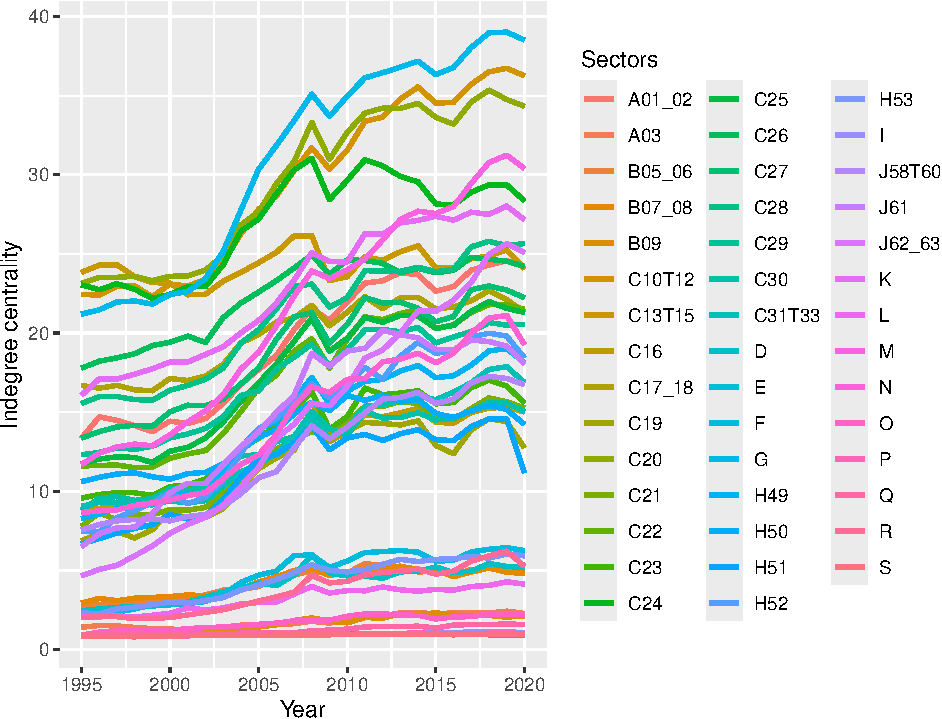
\includegraphics[width=0.49\linewidth]{sectp-1} }\subfloat[Outdegree centrality\label{fig:sectp-2}]{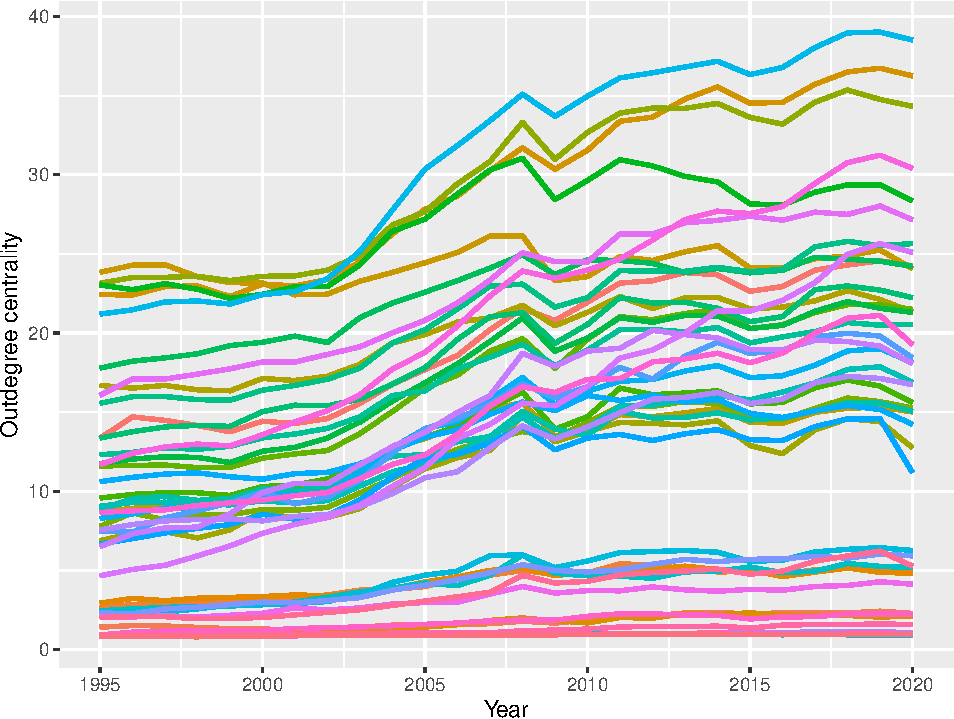
\includegraphics[width=0.49\linewidth]{sectp-2} }\newline\subfloat[Homophily\label{fig:sectp-3}]{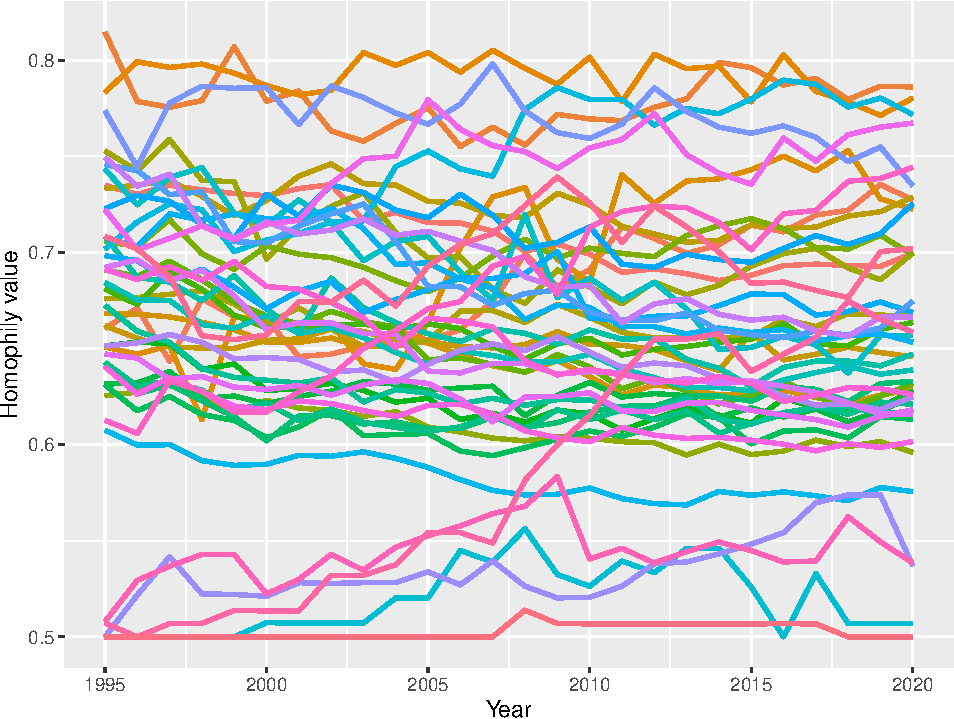
\includegraphics[width=0.49\linewidth]{sectp-3} }\subfloat[Leiden's modularity\label{fig:sectp-4}]{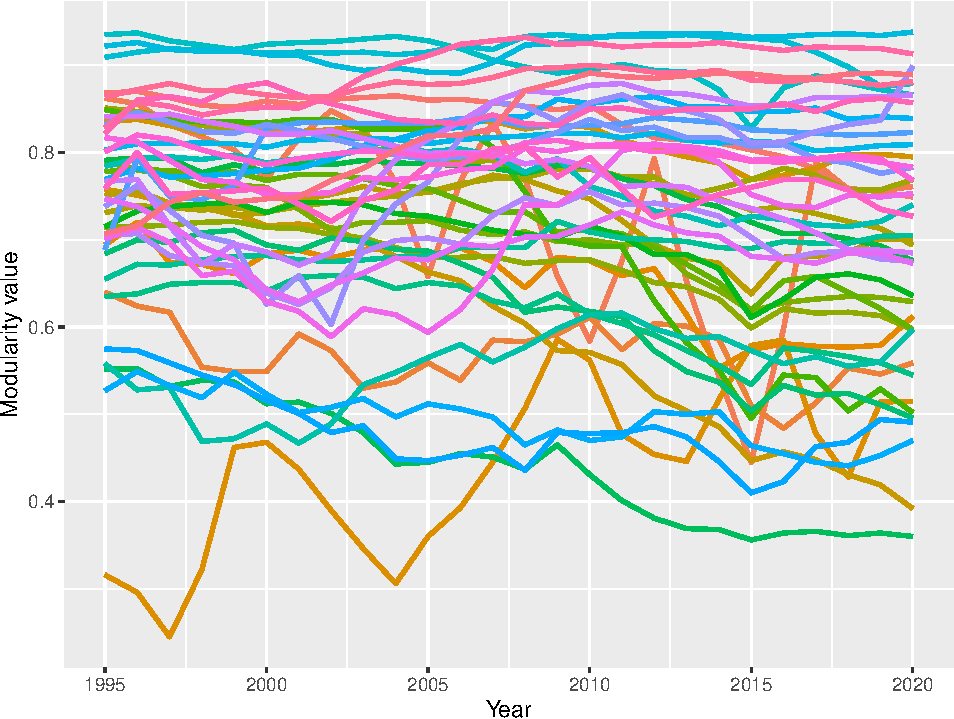
\includegraphics[width=0.49\linewidth]{sectp-4} }\newline\subfloat[Sectorial added vales (VAs)\label{fig:sectp-5}]{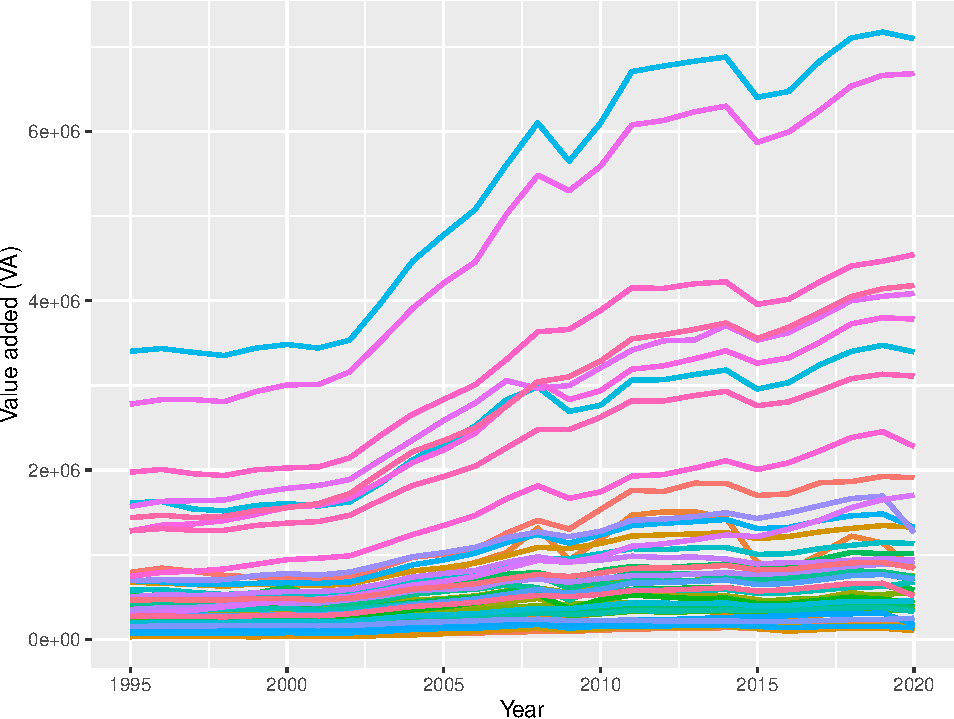
\includegraphics[width=0.49\linewidth]{sectp-5} }

}

\caption{Sectorial network properties}\label{fig:sectp}
\end{figure}
\begin{figure}[H]

{\centering \subfloat[Degree centralizations\label{fig:bayesnetwp-1}]{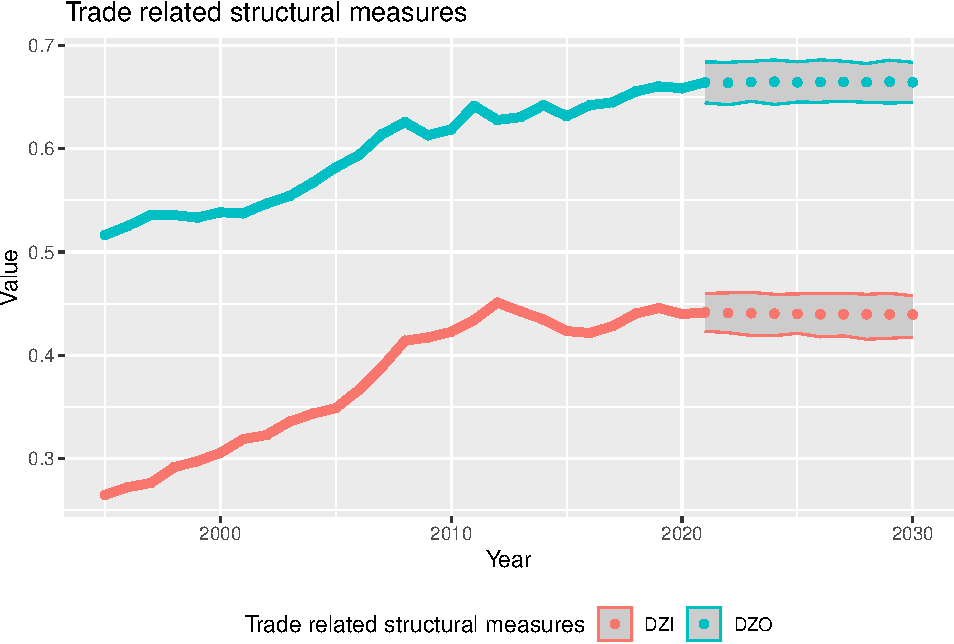
\includegraphics[width=0.33\linewidth]{bayesnetwp-1} }\subfloat[Resilience for random and systematic attacks\label{fig:bayesnetwp-2}]{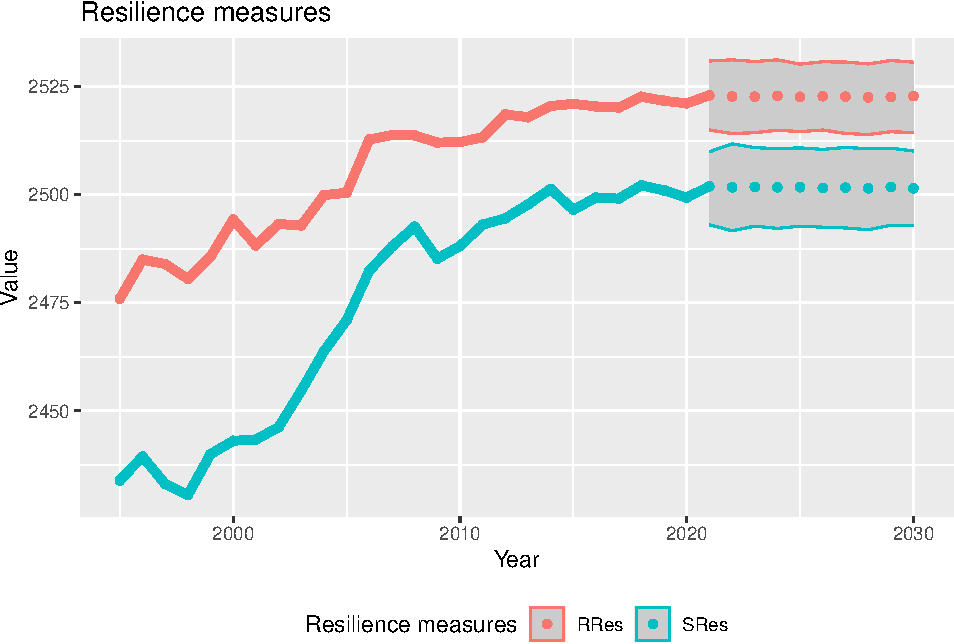
\includegraphics[width=0.33\linewidth]{bayesnetwp-2} }\subfloat[Average and global local efficiency and transitivity\label{fig:bayesnetwp-3}]{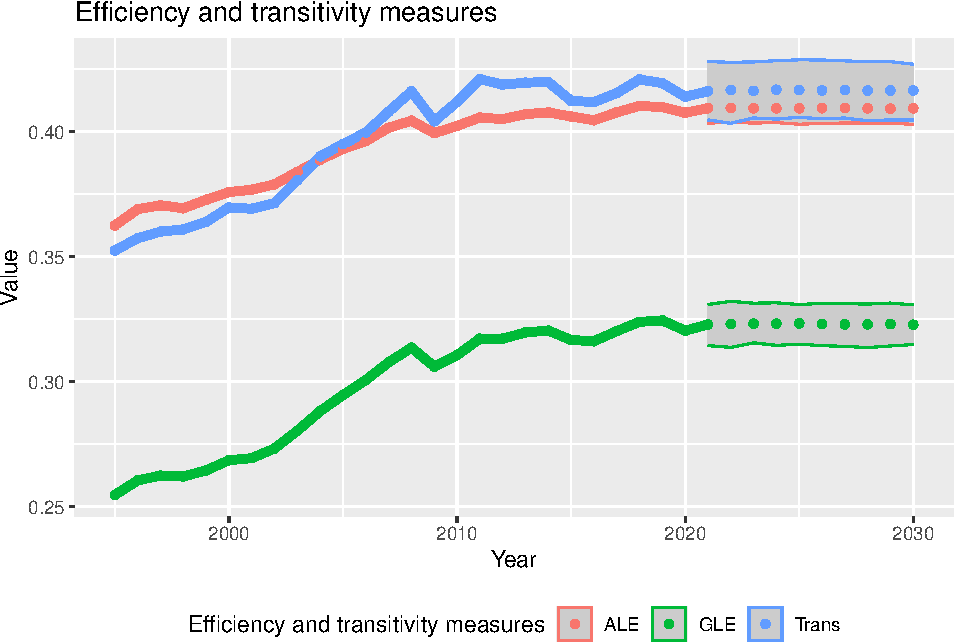
\includegraphics[width=0.33\linewidth]{bayesnetwp-3} }\newline\subfloat[PageRank centralizations and reach club cefficients\label{fig:bayesnetwp-4}]{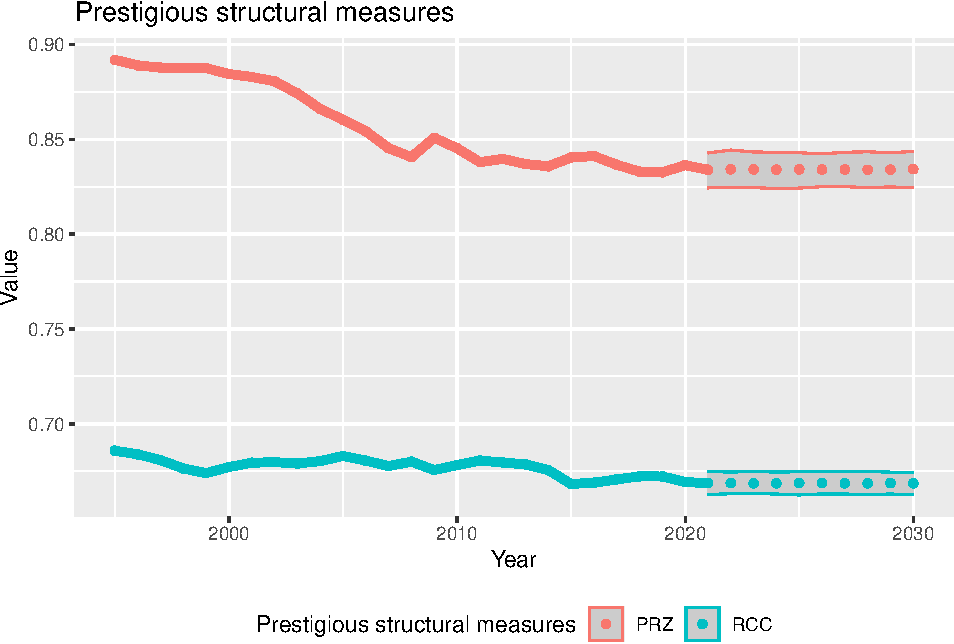
\includegraphics[width=0.33\linewidth]{bayesnetwp-4} }\subfloat[Modularity measures\label{fig:bayesnetwp-5}]{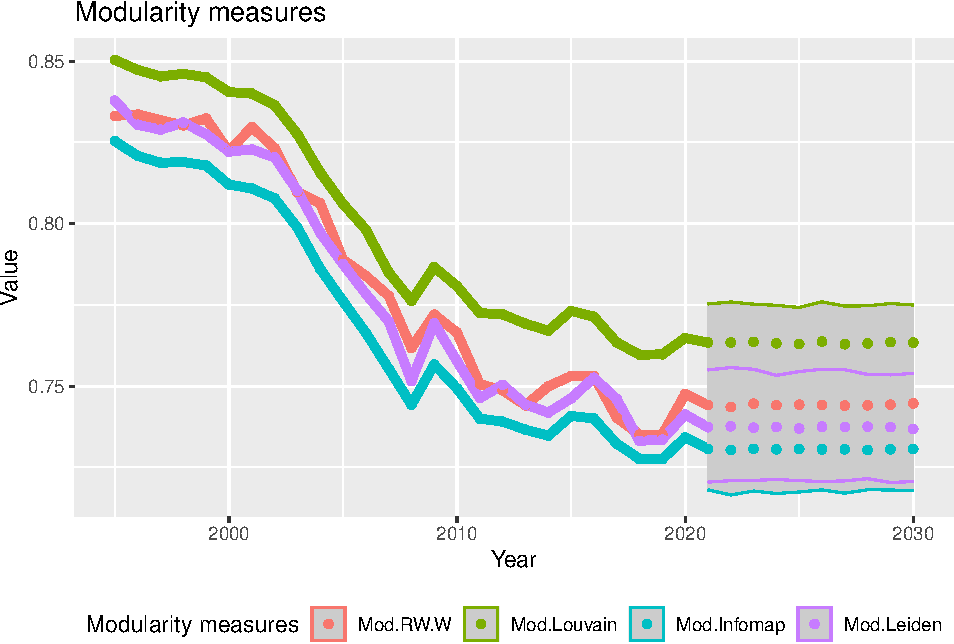
\includegraphics[width=0.33\linewidth]{bayesnetwp-5} }\subfloat[Average aggregated and multilayer path lengths\label{fig:bayesnetwp-6}]{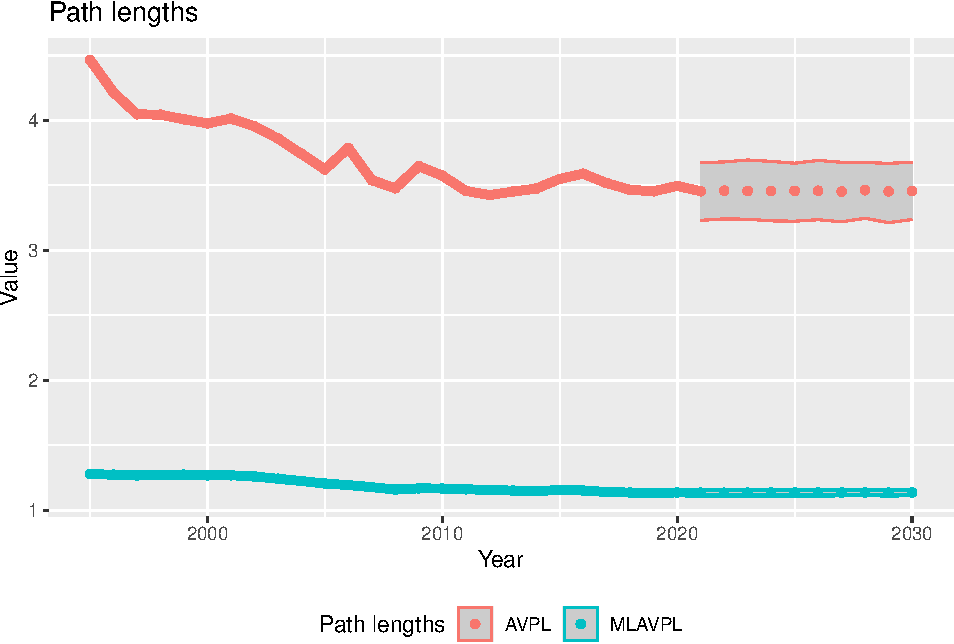
\includegraphics[width=0.33\linewidth]{bayesnetwp-6} }\newline\subfloat[Density, asymmetry and assortativity\label{fig:bayesnetwp-7}]{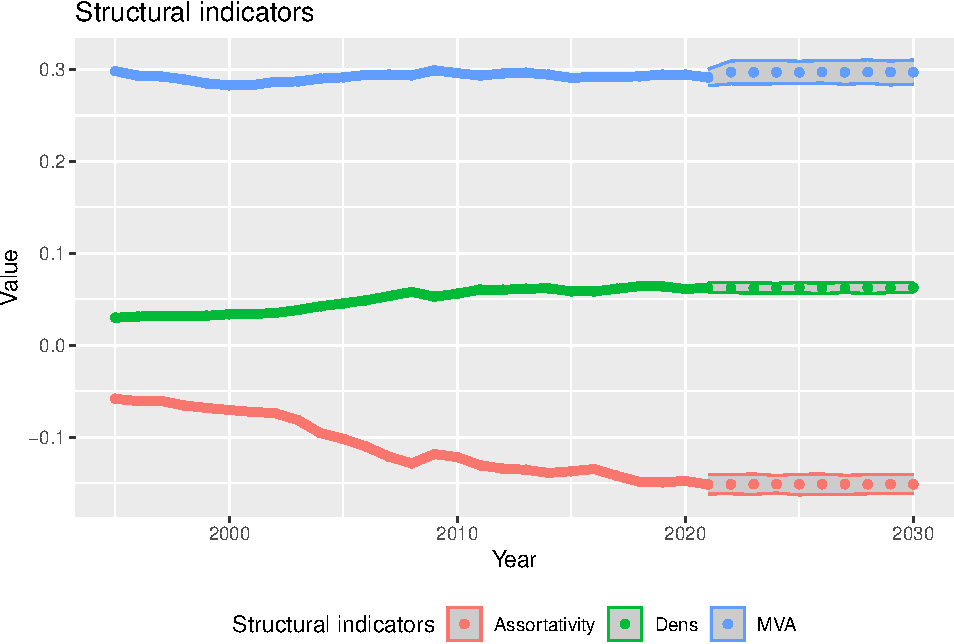
\includegraphics[width=0.33\linewidth]{bayesnetwp-7} }\subfloat[Betweennes and closeness centralizations\label{fig:bayesnetwp-8}]{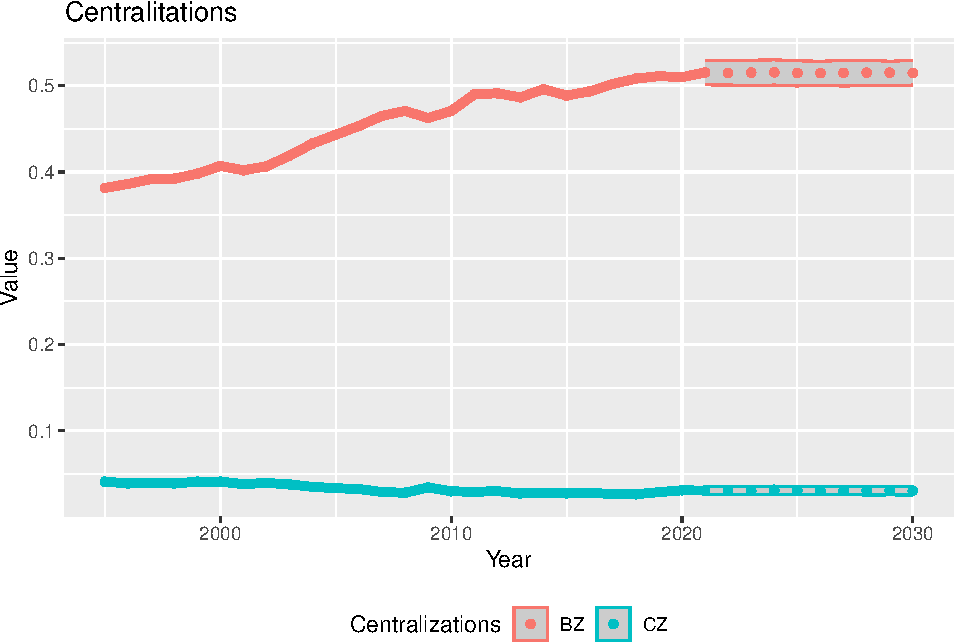
\includegraphics[width=0.33\linewidth]{bayesnetwp-8} }\subfloat[Average similarity values\label{fig:bayesnetwp-9}]{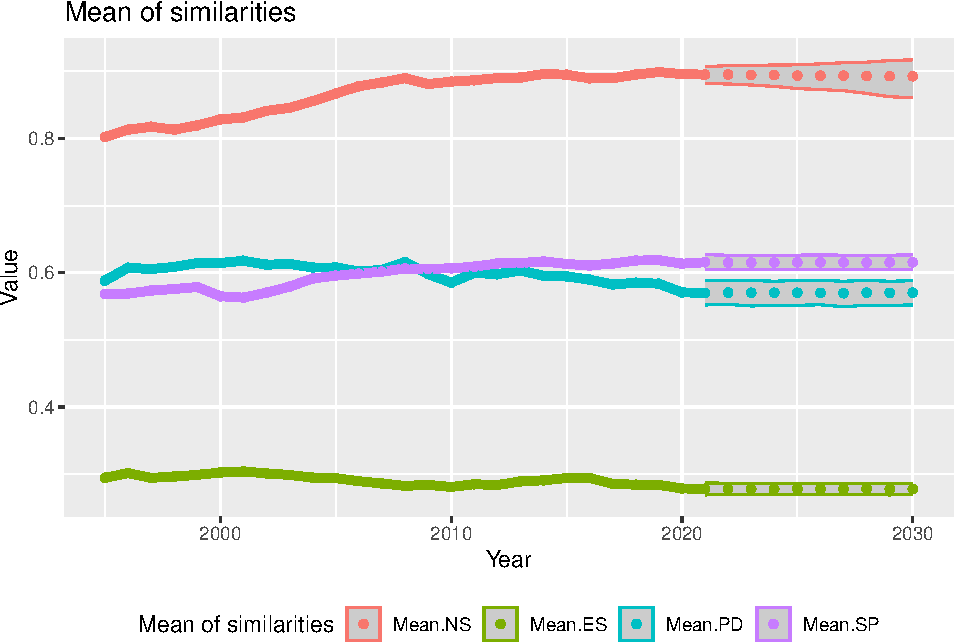
\includegraphics[width=0.33\linewidth]{bayesnetwp-9} }\newline

}

\caption{Network properties in time (forecast wth Bayesian ARIMA, 95\% confidence interval)}\label{fig:bayesnetwp}
\end{figure}

\begin{figure}[H]

{\centering \subfloat[Outdegree centrality\label{fig:bayessectpnda-1}]{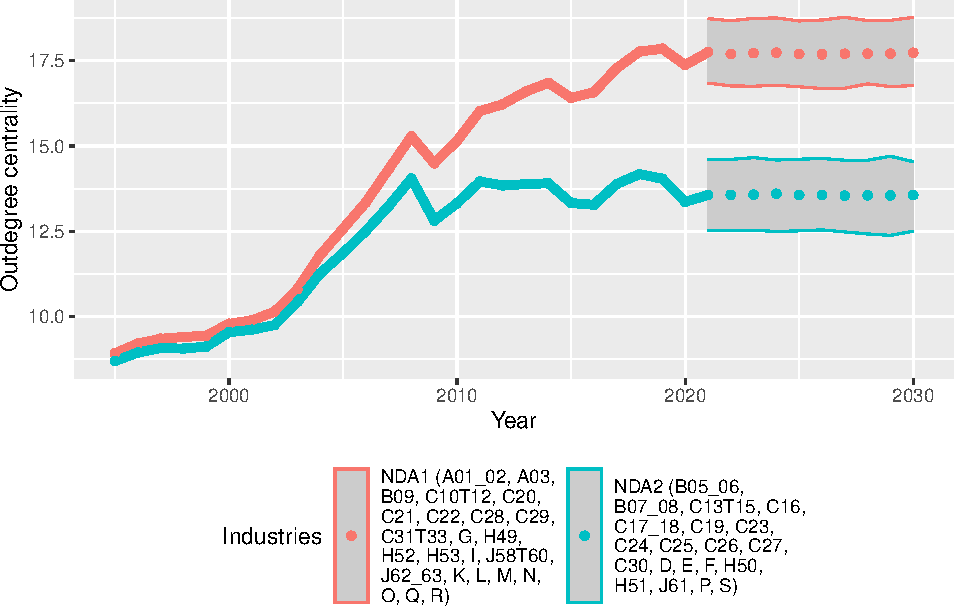
\includegraphics[width=0.33\linewidth]{bayessectpnda-1} }\subfloat[Homophily\label{fig:bayessectpnda-2}]{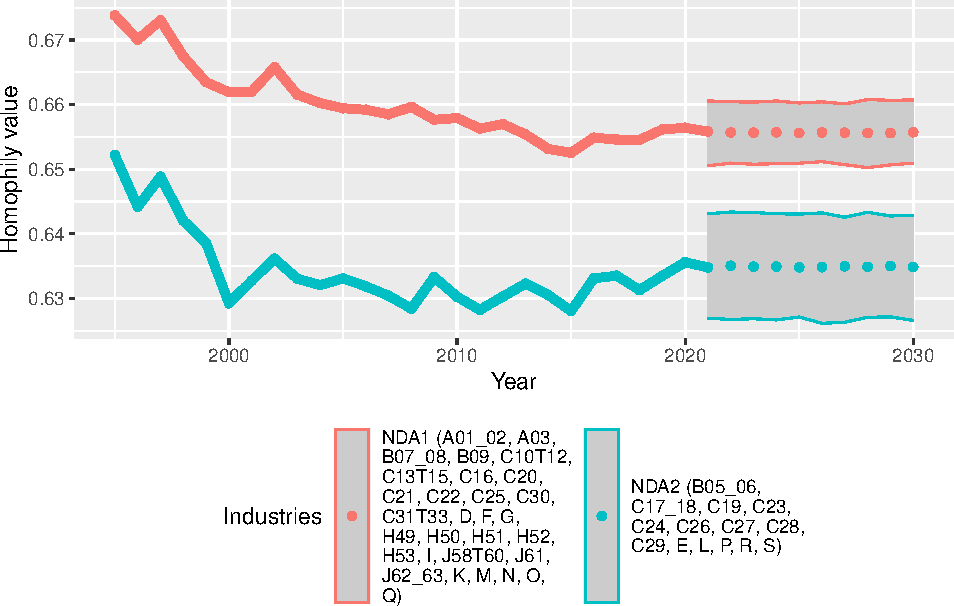
\includegraphics[width=0.33\linewidth]{bayessectpnda-2} }\subfloat[Leiden's modularity\label{fig:bayessectpnda-3}]{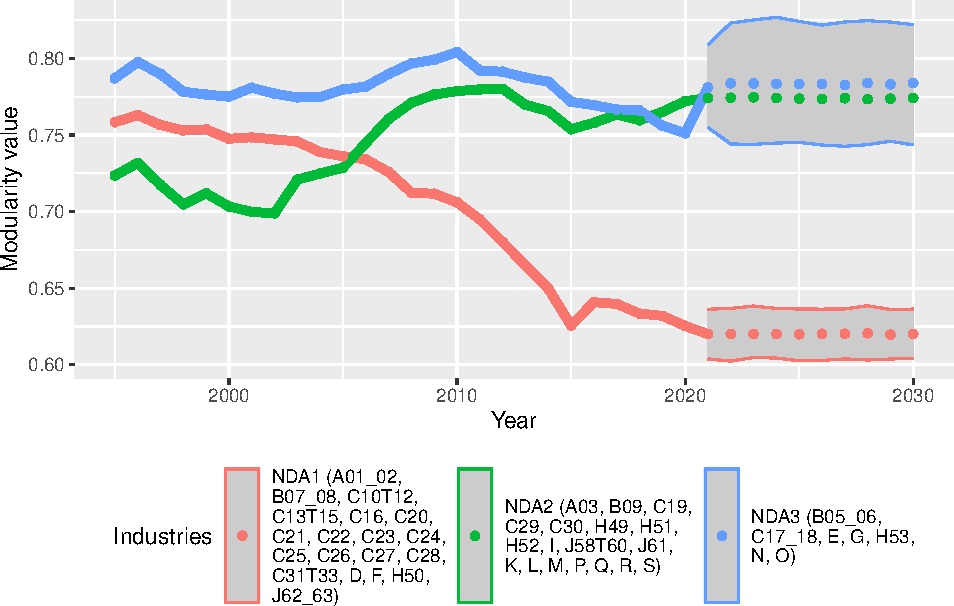
\includegraphics[width=0.33\linewidth]{bayessectpnda-3} }\newline\subfloat[Eigenvector centrality\label{fig:bayessectpnda-4}]{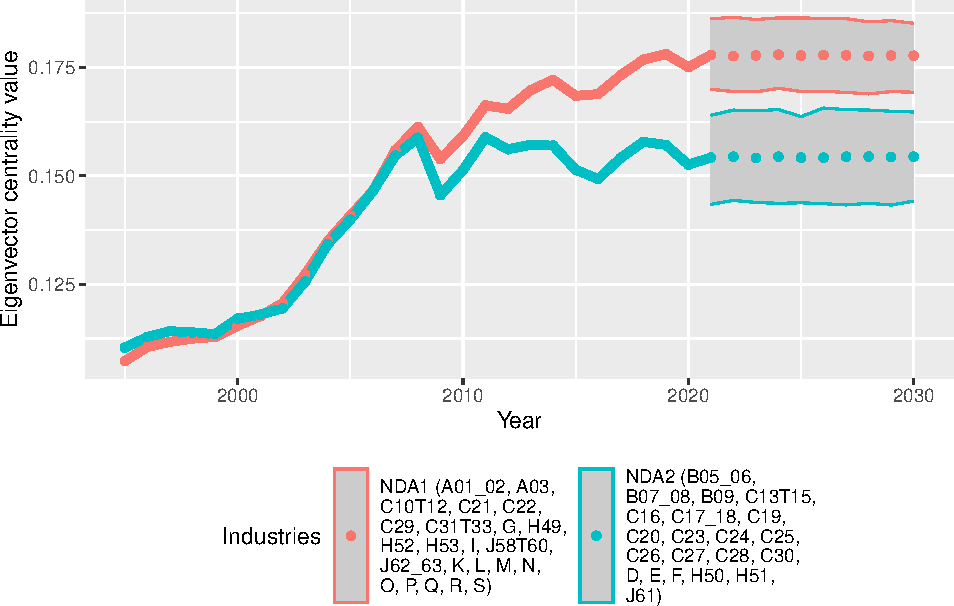
\includegraphics[width=0.33\linewidth]{bayessectpnda-4} }\subfloat[PageRank centrality\label{fig:bayessectpnda-5}]{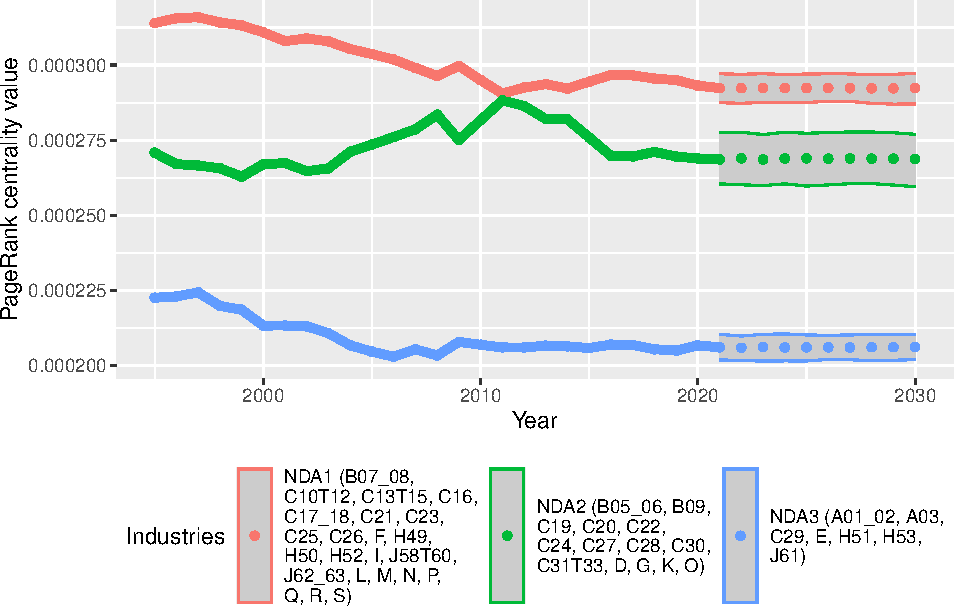
\includegraphics[width=0.33\linewidth]{bayessectpnda-5} }\subfloat[Betweenness centrality\label{fig:bayessectpnda-6}]{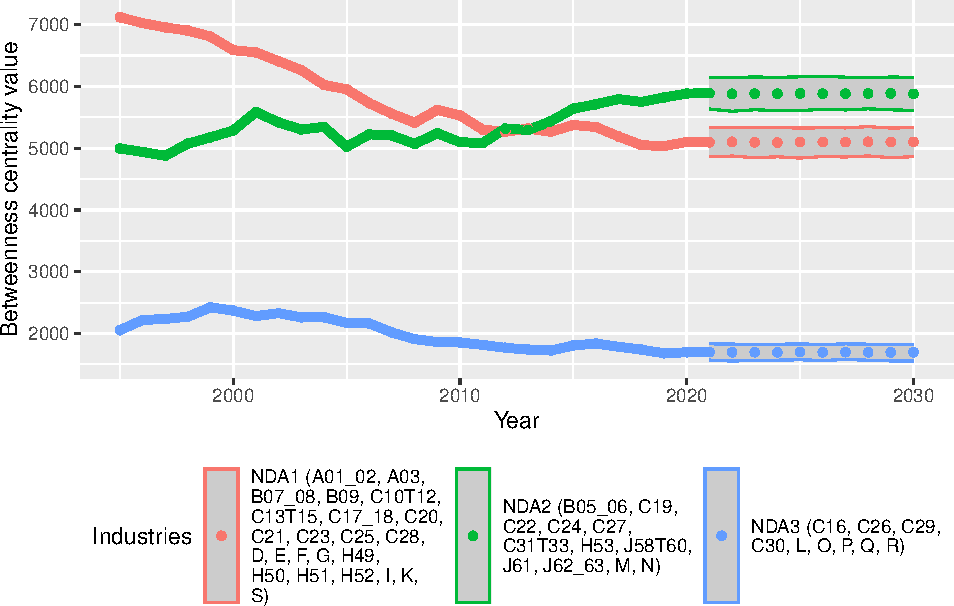
\includegraphics[width=0.33\linewidth]{bayessectpnda-6} }\newline\subfloat[Added values (VAs)\label{fig:bayessectpnda-7}]{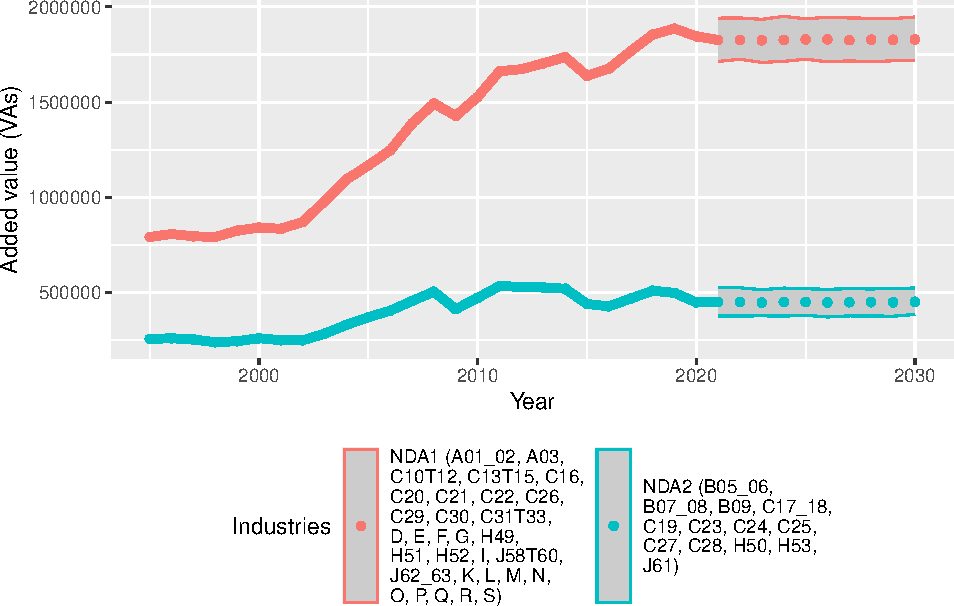
\includegraphics[width=0.33\linewidth]{bayessectpnda-7} }

}

\caption{Average clustered industrial node-level properties forecasting by Bayesian ARIMA models}\label{fig:bayessectpnda}
\end{figure}

\printglossaries

\section{List of Employed Node-Level
Indicators}\label{list-of-employed-node-level-indicators}

Table \ref{tab:nodeprop} shows the employed node-level centrality
measures, for a given (fixed) year.

\begin{table}[H]
    \centering
    \caption{Empployed node-level indicators in the multilayer trade network}
    \label{tab:nodeprop}
    \resizebox{\textwidth}{!}{
    \begin{tabular}{lp{2cm}lp{7cm}}
        \toprule
        \textbf{Abbr.} & \textbf{Node-Level Indicator} & \textbf{Formula} & Meanings\\ \midrule
        DCI & Indegree centrality & $DCI(c_{jq}) = \sum_{c_{ip} \in V} e_{ip,jq}$ & The number of exporters to country $j$ in industry $q$.\\
        DCO & Outdegree centrality & $DCO(c_{jq}) = \sum_{c_{ip} \in V} e_{jq,ip}$ & The number of importers from country $j$ in industry $q$.\\
        DC & Degree centrality & $DC(c_{jq}) = DCI(c_{jq})+DCO(c_{jq})$ & The number of trade partners of country $j$ in industry $q$.\\
        SCI & Instrength centrality & $SCI(c_{jq}) = \sum_{c_{ip} \in V} w(e_{ip,jq})$ & The volume of exports to country $j$ in industry $q$.\\
        SCO & Outstrength centrality & $SCO(c_{jq}) = \sum_{c_{ip} \in V} w(e_{jq,ip})$ & The volume of imports from country $j$ in industry $q$.\\
        BC  & Betweenness centrality & $BC(c_{jq}) = \sum_{c_{ip} \neq c_{jq} \neq c_{kr}} \frac{\sigma_{i,k}(c_{jp})}{\sigma_{i,k}}$ & Which a country acts as a bridge along the shortest paths between other countries in the trade network.\\
        CC  & Closeness centrality & $CC(c_{jq}) = \frac{1}{\sum_{c_{ip}(t) \in V} d({c_{jq},c_{ip}})}$ & How quickly a country can access other countries in the trade network based on the shortest paths.\\
         EC  & Eigenvector centrality & $EC(c_{jq}) = \frac{1}{\lambda} \sum_{c_{ip} \in V} w(e_{ip,jq}) EC(c_{ip})$ & Country’s influence in the trade network by considering not just the number of connections but the importance of those connections.\\
        AUT & Authority centrality & $AUT(c_{jq}) = \sum_{c_{ip} \in V} HUB(c_{ip})$ & The country's reputation or significance as a trusted source of exports within a particular industry. High authority scores indicate that a country is seen as a primary destination for trade.\\
        HUB & Hubness centrality & $HUB(c_{jq}) = \sum_{c_{ip} \in V} AUT(c_{ip})$ & The ability of a country to direct trade toward other significant trading partners.\\
        PRC & PageRank centrality & $PRC(c_{jq}) = (1 - d) + d \sum_{c_{ip} \in V} \frac{PRC(c_{ip})}{DCO(c_{ip})}$ & The importance of a country based on the trade volume and connectivity of its trading partners. \\ 
        HOM & Homophily & $HOM_{jq}^C=C(c_{jq})\%=\frac{C(c_{jq})|_{l_q}}{C(c_{jq})}$ & Relative centrality value restricted to industry $q$.\\ \bottomrule
    \end{tabular}}
\end{table}

\noindent where \(\sigma_{i,k}(c_{jp})\) is the number of shortest paths
between nodes \(c_{ip}\) and \(c_{kr}\) that pass through node
\(c_{jq}\). \(\sigma_{i,k}\) is the total number of shortest paths
between countries \(a_i\) and \(a_k\); \(d(c_{jq},c_{ip})\) is the
shortest distance from country \(j\) in industry \(q\) to country \(i\)
in industry \(p\); \(\lambda\) is the eigenvalue of the adjacency matrix
used to compute eigenvector centrality; \(d\) is a damping factor used
in PageRank calculations, typically set to around 0.85; \(HOM_{jq}^C\)
is a relative centrality or Homophily measure for a given centrlity
measure \(C\) for country \(j\) in industry \(q\), \(C(c_{jq})|_{l_q}\)
is a given centrality measure restricted to the industry \(q\);
\(C(c_{jq})\) is an arbitrary centrality value without any industrial
restriction.

\section{Employed network-level
indicators}\label{employed-network-level-indicators}

Table \ref{tab:netwprop} lists the employed network-level indicators for
a fixed year.

\begin{table}[H]
    \centering
    \caption{Network-level indicators in the multilayer trade network}
    \label{tab:netwprop}
    \resizebox{\textwidth}{!}{
    \begin{tabular}{lp{2cm}lp{7cm}}
        \toprule
        \textbf{Abbr.} & \textbf{Network-Level Indicator} & \textbf{Short Mathematical Formula} & \textbf{Interpretation} \\ \midrule
        Assort & Assortativity & $Assort = \frac{ \sum_{ip} (DC(c_{ip}) \cdot DC(c_jq)) - \frac{1}{M} \left( \sum_{ip} (DC(c_{ip}) \right)^2 }{ \frac{1}{M} \sum_{i} (DC(c_{ip})^2 - \frac{1}{E} \left( \sum_{ip} (DC(c_{ip}) \right)^2 }$ & Describes the tendency of countries to connect with others that have similar trade volumes or degrees, indicating whether trade relationships promote balance or disparity.  \\
         Dens & Density & $Dens = \frac{M}{N(N-1)}$ & Quantifies the proportion of possible trade connections that are realized, indicating how interconnected the countries are overall. \\ 
        AVPL & Average Path Length & $AVPL = \frac{1}{N(N-1)} \sum_{c_{ip} \neq c_{jq}} d(c_{ip}, c_{jq})$ & Represents the average number of steps needed to connect any two countries, reflecting the efficiency of trade routes. \\ 
        MLAVPL & Multilayer Average Path Length & $MLAVPL = \frac{1}{\sum_k |L_k|} \sum_{k} AVPL^{l_k}$ & Assessing the average path length across multiple layers shows how efficiently connections can be made through different industries. \\ 
        Tra & Transitivity & $Tra = \frac{3 \times \text{Triangles}}{\text{Connected triplets}}$ & Indicates the likelihood that countries sharing a common trading partner also trade with each other, reflecting the degree of clustering in trade relationships. \\ 
        DZI & Indegree centralization & $DZI = \frac{1}{N-1} \left( \frac{\sum_{ip}(DCI(c_{ip}) - DCI_{max})}{(N-1)(DCI_{max} - DCI_{min})} \right)$ & Measures the inequality in the incoming trade connections across countries, indicating dependence on a few major importers. \\ 
        DZO & Outdegree Centralization & $DZO = \frac{1}{N-1} \left( \frac{\sum_{ip}(DCO(c_{ip}) - DCO_{max})}{(N-1)(DCO_{max} - DCO_{min})} \right)$ & Indicates how concentrated outgoing trade relationships are, reflecting how few countries dominate as exporters. \\ 
        BZ  & Betweenness Centralization & $BZ = \frac{1}{(N-1)(N-2)} \sum_{ip} BC(c_{ip})$ & Highlights the extent to which countries act as intermediaries in trade, facilitating connections between others and controlling trade flows. \\ 
        CZ  & Closeness Centralization & $CZ = \frac{1}{N} \sum_{ip} CC(c_{ip})$ & Reflects the overall accessibility of countries to each other in the network, indicating the efficiency of trade connections. \\ 
        PRZ & PageRank Centralization & $PRZ = \frac{1}{N} \sum_{ip} PRC(c_{ip})$ & Measures the overall influence of countries based on their trade volume and the significance of their trading partners. \\ 
        MVA & Mean Vertex Asymmetries & $MVA = \frac{1}{N} \sum_{ip} |DCI(c_{ip}) - DCO(c_{ip})|$ & Provides insights into the balance between imports and exports across countries, highlighting structural inequalities in trade. \\ 
        RRes, SRes & Resilience for Random/ Systematic Attack & $\sum_pN_{p}^{retain}$ & Measures the ability of the network to maintain connectivity under random/systematic removals of countries, indicating robustness of trade relationships. \\ 
        Mod & Modularity Value & $Mod = \frac{1}{2M} \sum_{ip,jq} (A_{ip,jq} - DCI(c_{ip}) DCO(c_{jq})) \delta(C_i, C_j)$ & Identifies the degree to which the network can be divided into modules, or communities, with dense internal connections and sparse external ones, indicating trade groupings. \\ 
        RCC & Reach Club Coefficient & $RCC = \frac{1}{N} \sum_{ip} |N_{ip}|$ & Measures the efficiency of trade reachability across the network, indicating how well countries can connect with each other. \\ 
        MLGLClu & Multilayer Global Clustering & $MLGLClu = \frac{1}{M} \sum_{p} Clu^{p}$ & Captures the clustering tendency across different industries, reflecting the propensity for countries to develop strong trade ties within and between layers. \\ \bottomrule
    \end{tabular}}
\end{table}

\noindent  where \(N\) is the total number of nodes (countries), \(M\)
is the total number of edges, \(N_{p}^{\text{retain}}\) is the number of
nodes in the largest component in sector \(p\), \(A_{ip,jq}\) is the
(supra) adjacency matrix entry indicating connections between nodes
\(i\) and \(j\) in sector \(p\) and sector \(q\), \(|N_{ip}|\) is the
number of reachable nodes from node \(i\) in sector \(p\), and
\(Clu^{p}\) is the clustering coefficient in industry \(p\).

\section{The setting of ARIMA and causality
analysis}\label{sec:settingarima}

The \gls{arima} model is a widely used statistical technique for
forecasting time-series data. The \gls{arima} model is characterized by
three parameters -- \((p, d, q)\), where \(p\) is the number of
autoregressive terms, \(d\) is the degree of differencing needed to make
the time series stationary, and \(q\) is the number of lagged forecast
errors in the prediction equation. The general formulation of the
\gls{arima} model can be expressed as:

\begin{equation}
\Phi(B) (1 - B)^d y_t = \Theta(B) \epsilon_t
\end{equation}

\noindent where \(y_t\) represents the time series data, \(B\) is the
backshift operator, \(\Phi(B)\) is the autoregressive polynomial of
order \(p\), \((1 - B)^d\) signifies the differencing operation (where
\(d\) represents the number of differences taken to achieve
stationarity), \(\Theta(B)\) is the moving average polynomial of order
\(q\), and \(\epsilon_t\) denotes white noise error terms. By
identifying appropriate values for \(p\), \(d\), and \(q\) through the
analysis of \gls{acf} and \gls{pacf}, one can construct an optimal
\gls{arima} model tailored to the characteristics of the time series
data.

Prior to applying the \gls{arima} model, ensuring that the time series
data is stationary. Therefore, we assessed the results through tests
such as the \gls{adf} test, which examines the null hypothesis that a
unit root is present in the time series. If the p-value obtained from
the \gls{adf} test is below a predetermined significance level (commonly
0.05), the null hypothesis can be rejected, indicating that the series
is stationary. If the data require differencing (i.e., \(d > 0\)), this
process is usually repeated until a suitable level of stationarity is
achieved. Following differencing, diagnostic checks using the \gls{acf}
and \gls{pacf} plots help in identifying the optimal parameters \(p\)
and \(q\). Finally, model validation can be performed using metrics such
as the \gls{aic} or the \gls{bic}, along with residual analysis to
ensure the reliability and robustness of the \gls{arima} model. The
parameters of the \gls{arima} model were determined by the
\texttt{auto.arima} function of the \texttt{forecast} package. However,
the \gls{acf} and \gls{pacf} values and the stationarity of the time
series were also double checked. Stationarity was tested using \gls{adf}
tests, while the terms were determined using \gls{acf} and \gls{pacf}
functions.

The objective of investigating causal relationships is to determine how
alterations in the structure of the trade network or the roles of
countries and industries influence other entities over time. The
employed Granger causality, a concept named after the econometrician
Clive Granger \citep{granger1969investigating}, refers to a statistical
hypothesis test that determines whether one time series can predict
other time series on the basis of their historical values. Formally,
time series \(Y\) is said to \emph{Granger-cause} time series \(X\) if
past values of \(Y\) provide significant information about future values
of \(X\), given that past values of \(X\) alone do not provide the same
level of predictive power. This can be mathematically expressed in a
\gls{var} framework, where one might quantify the relationship as
follows:

\begin{eqnarray}
X_t = a_0 + \sum_{i=1}^{p} a_i X_{t-i} + \sum_{j=1}^{q} b_j Y_{t-j} + \epsilon_t\\
Y_t = c_0 + \sum_{i=1}^{p} c_i Y_{t-i} + \sum_{j=1}^{q} d_j X_{t-j} + \eta_t
\end{eqnarray}

If the coefficients \(b_j\) are statistically significant, we can
conclude that \(Y\) Granger-causes \(X\). A key aspect of Granger
causality is that it does not imply true causality in the philosophical
sense; rather, it establishes a \emph{predictive relationship} on the
basis of temporal precedence. Therefore, we use the precedence between
time series rather than causality relationships.

To select the appropriate lag for Granger causality testing, several
methods such as \gls{aic}, \gls{bic}, or \gls{sc} were employed and it
is tested with \gls{bvar} methods. These criteria evaluate the goodness
of fit of models with varying lags, penalizing for complexity to prevent
overfitting. Additionally, an F test was used to ascertain the
significance of the Granger causality results at different lag
structures, ensuring that one appropriately captures the underlying
temporal dynamics. To cross-validate the results and lags of Granger
causality analysis we also calculated several Bayesian approaches.

The \gls{bvar} method employs a structured prior distribution to address
the curse of dimensionality in multivariate time series models. For a
bivariate VAR(p) model
\(\mathbf{y}_t = \mathbf{c} + \sum_{i=1}^{p} \mathbf{A}_i \mathbf{y}_{t-i} + \boldsymbol{\epsilon}_t\),
the Minnesota prior assumes that each variable follows a random walk,
with prior mean \(\mathbb{E}[A_{ij}^{(l)}] = \delta_i \delta_{ij}\)
where \(\delta_i = 1\) and \(\delta_{ij}\) is the Kronecker delta. The
prior covariance structure is
\(\text{Var}[A_{ij}^{(l)}] = \frac{\lambda^2}{l^2} \frac{\sigma_i^2}{\sigma_j^2}\),
where \(\lambda\) controls overall tightness and \(l\) represents the
lag order. This method provides stable parameter estimates even with
limited data by shrinking coefficients toward economically meaningful
values, making it particularly suitable for Granger causality analysis
where parameter precision is crucial for reliable inference.

The \gls{mcmc} approach provides full posterior distributions for all
parameters through Gibbs sampling, offering comprehensive uncertainty
quantification. For the \gls{var} system
\(\mathbf{Y} = \mathbf{X}\boldsymbol{\beta} + \mathbf{E}\) where
\(\mathbf{E} \sim MN(\mathbf{0}, \boldsymbol{\Sigma}, \mathbf{I}_T)\),
we specify the following conjugate priors
\(\boldsymbol{\beta} | \boldsymbol{\Sigma} \sim MN(\mathbf{B}_0, \boldsymbol{\Sigma}, \mathbf{V}_0)\)
and \(\boldsymbol{\Sigma} \sim IW(\mathbf{S}_0, \nu_0)\). The Gibbs
sampler alternates between drawing
\(\boldsymbol{\beta}^{(i)} | \boldsymbol{\Sigma}^{(i-1)}, \mathbf{Y} \sim MN(\hat{\mathbf{B}}, \boldsymbol{\Sigma}^{(i-1)}, \hat{\mathbf{V}})\)
and
\(\boldsymbol{\Sigma}^{(i)} | \boldsymbol{\beta}^{(i)}, \mathbf{Y} \sim IW(\hat{\mathbf{S}}, \hat{\nu})\),
where the hat notation denotes posterior parameters. Granger causality
is assessed by computing the posterior probability
\(P(\gamma_j \neq 0 | \mathbf{Y})\) for the coefficients of the causal
variable. This method captures the full parameter uncertainty and
provides probabilistic statements about causality relationships.

The \gls{bfa} method provides direct model comparison by computing the
ratio of marginal likelihoods between competing hypotheses. For testing
whether \(x_1\) Granger-causes \(x_2\), we compare models \(M_1\)
(unrestricted) and \(M_0\) (restricted) through
\(BF_{10} = \frac{p(\mathbf{y}_2 | M_1)}{p(\mathbf{y}_2 | M_0)}\), where
the marginal likelihood under conjugate Normal-Gamma priors is
\(p(\mathbf{y} | M) = \frac{\Gamma(\alpha_n)}{\Gamma(\alpha_0)} \frac{(\beta_0)^{\alpha_0}}{(\beta_n)^{\alpha_n}} \frac{|\mathbf{V}_n|^{1/2}}{|\mathbf{V}_0|^{1/2}} (2\pi)^{-T/2}\),
with \(\alpha_n = \alpha_0 + T/2\),
\(\beta_n = \beta_0 + \frac{1}{2}(\mathbf{y}^T\mathbf{y} + \mathbf{b}_0^T\mathbf{V}_0^{-1}\mathbf{b}_0 - \mathbf{b}_n^T\mathbf{V}_n^{-1}\mathbf{b}_n)\),
and \(\mathbf{V}_n^{-1} = \mathbf{V}_0^{-1} + \mathbf{X}^T\mathbf{X}\).
The posterior probability of causality is then
\(P(M_1 | \mathbf{y}) = \frac{BF_{10}}{1 + BF_{10}}\) assuming equal
prior model probabilities. This approach provides direct evidence
quantification for competing causal hypotheses.

The synergistic value of employing all four methods lies in their
complementary strengths and the robustness achieved through
methodological triangulation. Convergent results across frequentist and
Bayesian paradigms strengthen confidence in causal inferences, whereas
divergent results signal the need for deeper investigation. The
classical approach provides computational efficiency and familiar
statistical interpretation, while Bayesian methods offer richer
uncertainty characterization and more flexible modeling assumptions. The
\gls{bvar} method connects classical and fully Bayesian approaches,
offering improved finite-sample properties without the computational
intensity of \gls{mcmc}. The \gls{bfa} provides the most direct
hypothesis testing framework, yielding clear evidence statements about
relative model support. Together, these methods create a robust
analytical framework that captures different dimensions of statistical
evidence, computational efficiency, and interpretive clarity, ultimately
leading to more reliable and nuanced conclusions about causal
relationships in time series data.

To establish a strong consensus across the four methodological
approaches, we must first standardize the diverse outputs into a common
evidence scale \([0,1]\), where 0 indicates no evidence for causality
and 1 represents maximum evidence. Let \(E_i \in [0,1]\) denote the
standardized evidence measure from method \(i\), where
\(i \in \{1,2,3,4\}\) corresponds to \gls{bvar}, Classical \gls{var},
\gls{mcmc} analysis, Bayesian, and \gls{bfa} approaches, respectively.

For the Granger causality based on classical \gls{var} method, we
transform the p-value \(p\) using the monotonic transformation:
\begin{equation}
E_1 = 1 - p
\end{equation}

For the \gls{bvar}, we utilize the \gls{fevd} proportion
\(\phi \in [0,1]\) that variable \(x_1\) contributes to the variance of
variable \(x_2\) at horizon \(h\): \begin{equation}
E_2 = \frac{\text{FEVD}_{x_1 \rightarrow x_2}(h)}{\sum_{j} \text{FEVD}_{j \rightarrow x_2}(h)}
\end{equation}

For the \gls{mcmc} Bayesian method, we directly use the posterior
probability of causality: \begin{equation}
E_3 = P(\gamma \neq \mathbf{0} | \mathbf{Y})
\end{equation} where \(\gamma\) represents the vector of coefficients
for the causal variable in the target equation.

For the \gls{bfa}, we convert the Bayes factor \(BF_{10}\) to posterior
probability assuming equal prior model probabilities: \begin{equation}
E_4 = \frac{BF_{10}}{1 + BF_{10}}
\end{equation}

For the strong consensus, significant causality (\(p<0.01\)), high
posterior probability (\(Prob(>0.85)\)), strong \gls{fevd}
(\(FEVD>0.15\)), and strong \(BF_{10}>5\) were assumed Granger
causalitiy between two time series. This careful approach is essential
in economic modeling, where misidentified causal relationships could
lead to misguided policy recommendations or investment strategies.

Conversely, instantaneous causality is a more immediate concept, which
refers to the relationship between variables at the same point in time.
Such causality assesses whether two variables are correlated at a
specific moment, typically measured via correlation coefficients.
Mathematically, if two variables \(X_t\) and \(Y_t\) have their
correlation is expressed as follows:

\begin{equation}
cor(X_t, Y_t) = \frac{cov(X_t, Y_t)}{\sigma_{X} \sigma_{Y}}
\end{equation}

where \(cov\) denotes covariance and \(\sigma\) represents the standard
deviations of \(X\) and \(Y\), then, instantaneously, changes in one
variable may be associated with changes in the other variables at the
same time. Unlike Granger causality, instantaneous causality does not
attempt to evaluate the temporal influence of one variable on another
variable. When comparing the two concepts, Granger causality focuses on
the predictive capacity of a variable over time, whereas instantaneous
causality examines the correlation at a single point in time. Both
concepts can coexist in an analysis; one may find that two variables are
instantaneously correlated but does not exhibit a Granger-causal
relationship, indicating that while they move together, one does not
predict the other.

Despite their advantages, Granger causality and instantaneous causality
analyses have several limitations. These analyses assume linear
relationships between variables and can be sensitive to the choice of
lags and the presence of outliers. Furthermore, these analyses may lead
to spurious results in the presence of confounding variables or
nonstationary data, which necessitates pretesting for stationarity
through tests such as the \gls{adf} test. However, despite these
limitations, Granger causality and instantaneous causality can be
incredibly useful in analyzing a 26-year trade network in terms of
deriving insights into the dynamic relationships among trading
countries, industries, and economic indicators. By applying appropriate
preprocessing steps, such as differencing and cointegration analysis,
researchers can enrich their understanding of how trade dynamics change
over time and which factors truly influence these changes in a
temporally structured manner, shedding light on policy implications and
future trends in international trade. However, when analyzing relatively
short-term time-series data, such as a 26-year period (1995--2020),
Granger causality emerges as an ideal choice because advanced causality
methods require longer-term time series.

\section{The application of community-based clustering and biclustering
methods}\label{sec:settingcluster}

Modularity-based community detection algorithms minimize Eq.
\eqref{eq:modularity} as follows:

\begin{equation} \label{eq:modularity}
M = \frac{1}{2L} \displaystyle\sum_{i,j} \left(r_{i,j}- \gamma\hat{r}_{i,j}\right) \delta(C_i,C_j),
\end{equation}

\noindent  where \(M\) is the modularity value, \(r_{i,j}\) is the edge
weight between nodes \(i\) and \(j\), \(\hat{r}_{i,j}\) is the expected
weight based on the null model of \cite{newman2006modularity}, \(L\) is
the total weight in the network, \(\gamma\) is a constant (default 1),
and \(\delta\) equals 1 if nodes \(i\) and \(j\) belong to the same
community and 0 otherwise. For directed similarity graphs, Eq.
\eqref{eq:modularity_directed} must be minimized.

\begin{equation} \label{eq:modularity_directed}
M = \frac{1}{L} \displaystyle\sum_{i,j} \left(r_{i,j}- \gamma\hat{r}_{i,j}\right) \delta(C_i,C_j),
\end{equation}

The result of community detection is a partition of the graph. By
further developing this method, by specifying a given distance measure,
it is possible to search for modules and, thus, indicator groups between
variables and data \citep{kosztyan2022network}. This procedure is
adopted in the \gls{gnda} method, which does not require us to specify
the number of clusters in advance. In real and synthetic tests, the
method correctly estimated the number of clusters
\citep{kosztyan2024generalized}, and thus, we also used this approach to
separate the time series of industry patterns.

Conversely, biclustering goes a step further by allowing for The
simultaneous clustering of both rows and columns in an adjacency matrix,
a capability that is particularly useful when dealing with data that
have inherent multidimensional characteristics. In the context of a
directed trade network, where nodes represent various node or network
properties and edges signify the causal relationships between these
properties, biclustering can provide a more nuanced analysis. This
approach allows for the identification of subgroups of nodes that
exhibit similar behaviors or properties across specific conditions or
timeframes while also revealing which causal relationships (the edges)
are most significant within those groupings.

We employed the \gls{ibbig} method, which assumes that the utilized
dataset is binary.

This algorithm balances the homogeneity (in this case, entropy) of the
selected submatrix with the size of the league. Formally, the iBBiG
algorithm maximizes the following target function if the binarized
dataset with a given threshold \(tr\) is denoted as \(B_{tr}\):

\begin{equation}\label{eq:iBBiG}
    \max \leftarrow score:=(1-H_{\mathcal{B}})^{\alpha}\left\{
    \begin{array}{cl}
    \sum_{i}{\sum_{j}{[\mathcal{B}]_{i,j}}}&\textrm{, if }Me(\mathcal{B})>\tau\\
    0&\textrm{, if }Me(\mathcal{B})\leq \tau,
    \end{array}\right.
\end{equation}

\noindent  where \(score\) is the score value of the submatrix
(bicluster, league) \(\mathcal{B}\in B_{tr}\). \(H_{\mathcal{B}}\) is
the entropy of submatrix \(\mathcal{B}\), with a given threshold \(tr\),
\(Me(\mathcal{B})\) is the median of bicluster \(\mathcal{B}\),
\(\alpha \in[0,1]\) is the exponent, and \(\tau\) is the cutting value.
If \(tr, \tau\) or \(\alpha\) is increased, then we obtain a smaller but
more homogeneous submatrix. To strengthen the significance, stability
and reliability, previous studies
\citep[see, e.g.,][]{Gusenleitner2012iBBiG,kosztyanrankings2019}
recommend that the balance exponent (\(\alpha\)) be set to 0.3 while the
cutoff threshold (\(\tau\)) be set to 0.5.

Identifying biclusters is a heuristic method. Therefore, in addition to
conducting significance tests both for rows and columns, we must
calculate the stability of the biclusters. Typically, a bootstrapping
algorithm is used to calculate the stability of biclusters. This method
ignores rows and columns and evaluates the changes within biclusters
\citet{lee2011boostrap}. Stability is also calculated for both rows and
columns. We say that a bicluster is significant (stable) if it is
significant (stable) for both rows and columns. We calculated both the
significance and stability of each bicluster.

\section{List of employed similarity
indicators}\label{list-of-employed-similarity-indicators}

Table \ref{tab:sectorsim} lists the employed similarity measures
comparing industries.

\begin{table}[H]
    \centering
    \caption{Employed similarity measures in the multilayer trade network}
    \label{tab:sectorsim}
    \resizebox{\textwidth}{!}{
    \begin{tabular}{lp{2cm}lp{7cm}}
        \toprule
        \textbf{Abbrev.} & \textbf{Similarity indicator} & \textbf{Formula} & \textbf{Interpretation} \\ \midrule
        NS  & Node similarity & $NS(p,q) = \frac{1}{A}\sum_i\frac{|N(c_{ip}) \cap N(c_{iq})|}{|N(c_{ip}) \cup N(c_{iq})|}$ & Measures the extent to which a country share common neighbors in different industries, indicating their relational similarity based on direct trade links. \\ 
        ES  & Edge similarity & $ES(p,q) = \frac{1}{A}\sum_i\frac{|T(e_{ip}) \cap T(e_{iq})|}{|T(e_{ip}) \cup T(e_{iq})|}$ & Assesses the similarity between two edges based on their incident nodes and trade volumes, reflecting how closely two trade relationships mirror each other. \\ 
        PD  & Pearson correlation of degree centralities & $PD(p,q) = cor(DC(c_{ip}),DC(c_{iq}))$ & Examines the linear correlation between the degree centralities of countries across two different industries, indicating the consistency of trade relationships across those industries. \\ 
        SP  & Shortest path distances & $SP(p, q) = \frac{1}{A}\sum_i (\min \{d(c_{ip}, c_{iq})$ & Represents the minimum number of edges that must be traversed to connect two countries, highlighting the efficiency of trade routes and potential connectivity between them. \\ \bottomrule
    \end{tabular}}
\end{table}

\noindent  where \(A\) is the number of actors where each country is
considered only once. \(N(c_{ip})\) is the set of neighbors (trading
partners) for country \(i\) in industry \(p\), and \(T(e(i_p))\) is the
set of trade relations for edges \(e(i_p,i_q)\) and \(e(i_q,i_p)\).

\section{List of Country and Industrial
Codes}\label{list-of-country-and-industrial-codes}

\begin{table}[H]
\centering
\caption{\label{tab:countries}List of countries}
\centering
\fontsize{8}{10}\selectfont
\begin{tabular}[t]{>{}r|l>{}l||>{}r|ll}
\toprule
\textbf{ID} & \textbf{ISO3} & \textbf{Country} & \textbf{ID} & \textbf{ISO3} & \textbf{Country}\\
\midrule
\midrule
\textbf{1} & ARG & Argentina & \textbf{40} & KAZ & Kazakhstan\\
\textbf{2} & AUS & Australia & \textbf{41} & KHM & Cambodia\\
\textbf{3} & AUT & Austria & \textbf{42} & KOR & Korea\\
\textbf{4} & BEL & Belgium & \textbf{43} & LAO & Lao (People's Democratic Republic)\\
\textbf{5} & BGD & Bangladesh & \textbf{44} & LTU & Lithuania\\
\textbf{6} & BGR & Bulgaria & \textbf{45} & LUX & Luxembourg\\
\textbf{7} & BLR & Belarus & \textbf{46} & LVA & Latvia\\
\textbf{8} & BRA & Brazil & \textbf{47} & MAR & Morocco\\
\textbf{9} & BRN & Brunei Darussalam & \textbf{48} & MEX & Mexico\\
\textbf{10} & CAN & Canada & \textbf{49} & MLT & Malta\\
\textbf{11} & CHE & Switzerland & \textbf{50} & MMR & Myanmar\\
\textbf{12} & CHL & Chile & \textbf{51} & MYS & Malaysia\\
\textbf{13} & CHN & China (People's Republic of) & \textbf{52} & NGA & Nigeria\\
\textbf{14} & CIV & Côte d'Ivoire & \textbf{53} & NLD & Netherlands\\
\textbf{15} & CMR & Cameroon & \textbf{54} & NOR & Norway\\
\textbf{16} & COL & Colombia & \textbf{55} & NZL & New Zealand\\
\textbf{17} & CRI & Costa Rica & \textbf{56} & PAK & Pakistan\\
\textbf{18} & CYP & Cyprus & \textbf{57} & PER & Peru\\
\textbf{19} & CZE & Czechia & \textbf{58} & PHL & Philippines\\
\textbf{20} & DEU & Germany & \textbf{59} & POL & Poland\\
\textbf{21} & DNK & Denmark & \textbf{60} & PRT & Portugal\\
\textbf{22} & EGY & Egypt & \textbf{61} & ROU & Romania\\
\textbf{23} & ESP & Spain & \textbf{62} & RUS & Russian Federation\\
\textbf{24} & EST & Estonia & \textbf{63} & SAU & Saudi Arabia\\
\textbf{25} & FIN & Finland & \textbf{64} & SEN & Senegal\\
\textbf{26} & FRA & France & \textbf{65} & SGP & Singapore\\
\textbf{27} & GBR & United Kingdom & \textbf{66} & SVK & Slovakia\\
\textbf{28} & GRC & Greece & \textbf{67} & SVN & Slovenia\\
\textbf{29} & HKG & Hong Kong, China & \textbf{68} & SWE & Sweden\\
\textbf{30} & HRV & Croatia & \textbf{69} & THA & Thailand\\
\textbf{31} & HUN & Hungary & \textbf{70} & TUN & Tunisia\\
\textbf{32} & IDN & Indonesia & \textbf{71} & TUR & Turkey\\
\textbf{33} & IND & India & \textbf{72} & TWN & Chinese Taipei\\
\textbf{34} & IRL & Ireland & \textbf{73} & UKR & Ukraine\\
\textbf{35} & ISL & Iceland & \textbf{74} & USA & United States\\
\textbf{36} & ISR & Israel & \textbf{75} & VNM & Vietnam\\
\textbf{37} & ITA & Italy & \textbf{76} & ZAF & South Africa\\
\textbf{38} & JOR & Jordan & \textbf{77} & ROW & Rest of the World\\
\textbf{39} & JPN & Japan & \textbf{} &  & \\
\bottomrule
\end{tabular}
\end{table}

\begin{table}[H]
\centering
\caption{\label{tab:industries}List of industries (sectors)}
\centering
\fontsize{7}{9}\selectfont
\begin{tabu} to \linewidth {>{}r|>{\raggedright}X>{\raggedright}X>{\raggedright}X}
\toprule
\textbf{ID} & \textbf{Old code} & \textbf{Code} & \textbf{Industry}\\
\midrule
\midrule
\textbf{1} & D01T02 & A01\_02 & Agriculture, hunting, forestry\\
\textbf{2} & D03 & A03 & Fishing and aquaculture\\
\textbf{3} & D05T06 & B05\_06 & Mining and quarrying, energy producing products\\
\textbf{4} & D07T08 & B07\_08 & Mining and quarrying, non-energy producing products\\
\textbf{5} & D09 & B09 & Mining support service activities\\
\textbf{6} & D10T12 & C10T12 & Food products, beverages and tobacco\\
\textbf{7} & D13T15 & C13T15 & Textiles, textile products, leather and footwear\\
\textbf{8} & D16 & C16 & Wood and products of wood and cork\\
\textbf{9} & D17T18 & C17\_18 & Paper products and printing\\
\textbf{10} & D19 & C19 & Coke and refined petroleum products\\
\textbf{11} & D20 & C20 & Chemical and chemical products\\
\textbf{12} & D21 & C21 & Pharmaceuticals, medicinal chemical and botanical products\\
\textbf{13} & D22 & C22 & Rubber and plastics products\\
\textbf{14} & D23 & C23 & Other non-metallic mineral products\\
\textbf{15} & D24 & C24 & Basic metals\\
\textbf{16} & D25 & C25 & Fabricated metal products\\
\textbf{17} & D26 & C26 & Computer, electronic and optical equipment\\
\textbf{18} & D27 & C27 & Electrical equipment\\
\textbf{19} & D28 & C28 & Machinery and equipment, nec\\
\textbf{20} & D29 & C29 & Motor vehicles, trailers and semi-trailers\\
\textbf{21} & D30 & C30 & Other transport equipment\\
\textbf{22} & D31T33 & C31T33 & Manufacturing nec; repair and installation of machinery and equipment\\
\textbf{23} & D35 & D & Electricity, gas, steam and air conditioning supply\\
\textbf{24} & D36T39 & E & Water supply; sewerage, waste management and remediation activities\\
\textbf{25} & D41T43 & F & Construction\\
\textbf{26} & D45T47 & G & Wholesale and retail trade; repair of motor vehicles\\
\textbf{27} & D49 & H49 & Land transport and transport via pipelines\\
\textbf{28} & D50 & H50 & Water transport\\
\textbf{29} & D51 & H51 & Air transport\\
\textbf{30} & D52 & H52 & Warehousing and support activities for transportation\\
\textbf{31} & D53 & H53 & Postal and courier activities\\
\textbf{32} & D55T56 & I & Accommodation and food service activities\\
\textbf{33} & D58T60 & J58T60 & Publishing, audiovisual and broadcasting activities\\
\textbf{34} & D61 & J61 & Telecommunications\\
\textbf{35} & D62T63 & J62\_63 & IT and other information services\\
\textbf{36} & D64T66 & K & Financial and insurance activities\\
\textbf{37} & D68 & L & Real estate activities\\
\textbf{38} & D69T75 & M & Professional, scientific and technical activities\\
\textbf{39} & D77T82 & N & Administrative and support services\\
\textbf{40} & D84 & O & Public administration and defence; compulsory social security\\
\textbf{41} & D85 & P & Education\\
\textbf{42} & D86T88 & Q & Human health and social work activities\\
\textbf{43} & D90T93 & R & Arts, entertainment and recreation\\
\textbf{44} & D94T96 & S & Other service activities\\
\textbf{45} & D97T98 & T & Activities of households as employers; undifferentiated goods- and services-producing activities of households for own use\\
\bottomrule
\end{tabu}
\end{table}


\end{document}
